\documentclass[12pt,a4paper]{article}

%!TEX program = pdflatex

% =============================================================================
% 1. PHONG CHU & NGON NGU
% =============================================================================
\usepackage[utf8]{inputenc}
\usepackage[T5]{fontenc}
\usepackage[vietnamese]{babel}

% =============================================================================
% 2. BO CUC TRANG
% =============================================================================
\usepackage[margin=2.5cm]{geometry}
\usepackage{setspace}
\onehalfspacing

% =============================================================================
% 3. DO HOA & BIEU DO
% =============================================================================
\usepackage{graphicx}
\usepackage{tikz}
\usetikzlibrary{arrows.meta, positioning, shapes.geometric}
\graphicspath{{project-overview/}{chapter-3-requirements/}{functional-modeling/}{software-architecture/}{database-design/}{../section7/}}

% =============================================================================
% 4. BANG BIEU & DANH SACH
% =============================================================================
\usepackage{array}
\usepackage{booktabs}
\usepackage{multirow}
\usepackage{longtable}
\usepackage{float}
\usepackage{enumitem}
\usepackage{tabularx}
\usepackage{makecell}
\usepackage{colortbl}
\usepackage{etoolbox}
\usepackage{amssymb}

% =============================================================================
% 5. TIEN ICH VAN BAN & LIEN KET
% =============================================================================
\usepackage{xcolor}
\usepackage{titlesec}
\usepackage{tocloft}
\usepackage{xurl}
\usepackage{seqsplit}
\usepackage{hyperref}

\hypersetup{
    colorlinks=false,
    hidelinks,
    pdftitle={Báo cáo hoàn chỉnh Tutor Management System},
    pdfauthor={Nhóm thực hiện}
}

% =============================================================================
% 6. DINH DANG DOAN VAN & DANH SO MUC
% =============================================================================
\setlength{\parindent}{0pt}
\setlength{\parskip}{6pt}
\setcounter{secnumdepth}{5}

\renewcommand{\thesection}{\Roman{section}}
\renewcommand{\thesubsection}{\arabic{subsection}}
\renewcommand{\thesubsubsection}{\thesubsection.\arabic{subsubsection}}
\renewcommand{\theparagraph}{\thesubsubsection.\arabic{paragraph}}
\renewcommand{\thesubparagraph}{\theparagraph.\arabic{subparagraph}}

\titleformat{\section}{\large\bfseries}{\thesection.}{0.5em}{}
\titleformat{\subsection}{\normalsize\bfseries}{\thesubsection.}{0.5em}{}
\titleformat{\subsubsection}{\normalsize\itshape\bfseries}{\thesubsubsection.}{0.5em}{}
\titleformat{\paragraph}[block]{\normalsize\bfseries}{\theparagraph.}{0.5em}{}
\titlespacing*{\paragraph}{0pt}{6pt}{2pt}
\titleformat{\subparagraph}[block]{\normalsize\itshape\bfseries}{\thesubparagraph.}{0.5em}{}
\titlespacing*{\subparagraph}{0pt}{4pt}{2pt}

\renewcommand{\cftsecaftersnum}{.}
\renewcommand{\cftsubsecaftersnum}{.}
\renewcommand{\cftsubsubsecaftersnum}{.}

% =============================================================================
% 7. CUSTOM COMMANDS & COLUMN TYPES
% =============================================================================
\newcolumntype{C}[1]{>{\centering\arraybackslash}p{#1}}
\newcolumntype{L}[1]{>{\raggedright\arraybackslash}p{#1}}
\newcolumntype{Y}{>{\raggedright\arraybackslash}X}
\newcommand{\subsubsubsection}[1]{\paragraph{#1}}
\newcommand{\tablesetup}{\small\setlength{\tabcolsep}{3pt}\renewcommand{\arraystretch}{1.2}}
\newcommand{\code}[1]{{\ttfamily\seqsplit{#1}}}
\newcommand{\datetimeoffset}{\makecell{DATETIME\\OFFSET}}
\AtBeginEnvironment{longtable}{\small\setlength{\parskip}{0pt}\setlength{\tabcolsep}{3pt}\renewcommand{\arraystretch}{1.15}}

\definecolor{uitblue}{HTML}{0056A6}
\definecolor{uitlightblue}{HTML}{EEF7FF}
\newcommand{\uitlogo}{
\includegraphics[height=2.8cm]{assets/logo-uit.jpg}}

\tikzset{
    process/.style={ellipse, draw, minimum width=3cm, minimum height=1.5cm, align=center},
    entity/.style={rectangle, draw, minimum width=2.5cm, minimum height=1cm, align=center},
    datastore/.style={
        draw=none, align=center, minimum width=3cm,
        append after command={
            [shorten <= -0.2cm, shorten >= -0.2cm]
            (\tikzlastnode.north west) edge (\tikzlastnode.north east)
            (\tikzlastnode.south west) edge (\tikzlastnode.south east)
        }
    },
    arrow/.style={-Stealth, thick}
}

\newcommand{\dfddiagram}[4]{%
\par\noindent$\triangleright$ Sơ đồ luồng dữ liệu:
\begin{center}
\begin{tikzpicture}[
    font=\normalsize,
    dfdentity/.style={rectangle, draw=black, minimum width=2.7cm, minimum height=0.8cm, align=center, inner sep=3pt},
    dfdprocess/.style={ellipse, draw=black, minimum width=3.8cm, minimum height=1.18cm, align=center, inner sep=2pt},
    dfdarrow/.style={-{Triangle[open,length=7pt,width=8pt]}, line width=0.8pt, draw=black},
    dfdblue/.style={-{Triangle[open,length=7pt,width=8pt]}, line width=0.8pt, draw=blue!45},
    label/.style={font=\normalsize, text=black}
]
\node[dfdprocess] (process) at (0,0) {#1};
\node[dfdentity] (actor) at (0,2.35) {#2};
\node[dfdentity] (input) at (-4.25,0) {#3};
\node[dfdentity] (output) at (4.45,0) {Thiết bị xuất};
\draw[line width=0.8pt] (-2.0,-2.02) -- (2.0,-2.02);
\draw[line width=0.8pt] (-2.0,-2.70) -- (2.0,-2.70);
\node[align=center] at (0,-2.36) {Bộ nhớ phụ};
\draw[dfdarrow] (-0.72,1.94) -- node[label,left] {D1} (-0.72,0.63);
\draw[dfdblue] (0.72,0.63) -- node[label,right] {D6} (0.72,1.94);
\draw[dfdblue] (input.east) -- node[label,above] {D2} (process.west);
\draw[dfdarrow] (process.east) -- node[label,above] {D5} (output.west);
\draw[dfdarrow] (-0.72,-2.02) -- node[label,left] {D3} (-0.72,-0.63);
\draw[dfdarrow] (0.72,-0.63) -- node[label,right] {D4} (0.72,-2.02);
\end{tikzpicture}
\end{center}
}



\begin{document}

\begin{titlepage}
    \centering
    \begin{tikzpicture}[remember picture,overlay]
        \fill[uitlightblue] (current page.south west) rectangle (current page.north east);
        \draw[uitblue,line width=2pt]
            ([xshift=0.65cm,yshift=0.65cm]current page.south west)
            rectangle
            ([xshift=-0.65cm,yshift=-0.65cm]current page.north east);
    \end{tikzpicture}

    \vspace*{0.8cm}
    \begin{minipage}[c][0.86\textheight][c]{0.82\textwidth}
        \centering
        \uitlogo\\[0.8cm]

        {\Large \textbf{\textcolor{uitblue}{ĐẠI HỌC CÔNG NGHỆ THÔNG TIN}}}\\[0.15cm]
        {\large \textbf{ĐẠI HỌC QUỐC GIA TP.HCM}}\\[0.9cm]

        {\large \textbf{SE104 - NHẬP MÔN CÔNG NGHỆ PHẦN MỀM}}\\[0.5cm]

        \rule{0.72\textwidth}{0.7pt}\\[0.6cm]
        {\Large \textbf{HỆ THỐNG QUẢN LÝ}}\\[0.2cm]
        {\Large \textbf{LỚP HỌC LẬP TRÌNH THI ĐẤU}}\\[0.6cm]
        \rule{0.72\textwidth}{0.7pt}\\[1.2cm]

        {\large \textbf{Giáo viên: ThS. Đỗ Văn Tiến}}\\[1.2cm]

        {\large \textbf{Nhóm sinh viên thực hiện}}\\[0.45cm]
        \begin{tabular}{ll}
            Nguyễn Thành Sơn & 24521532\\
            Lê Quang Trung & 24521883\\
            Đinh Mạnh Hùng & 24520014\\
            Trần Vạn Tấn & 23521407\\
        \end{tabular}

        \vfill
        {\large \textbf{Lớp SE104.Q29}}\\
    \end{minipage}
\end{titlepage}

\tableofcontents
\newpage

\section{Tổng quan đề tài}

\subsection{Giới thiệu đề tài}

Trong hoạt động dạy học theo mô hình lớp nhỏ hoặc gia sư, giáo viên thường phải
quản lý đồng thời nhiều nhóm thông tin: danh sách học sinh, lớp học, lịch học,
buổi học thực tế, điểm danh, học phí, giao dịch tài chính và kết quả luyện tập.
Nếu các dữ liệu này được ghi nhận rời rạc bằng sổ tay, bảng tính hoặc tin nhắn
riêng lẻ, việc theo dõi tình hình học tập và vận hành lớp học dễ phát sinh sai
sót, trùng lặp và thiếu tính kịp thời.

Bên cạnh đó, nhiều hoạt động hỗ trợ học tập hiện nay diễn ra trên các nền tảng
ngoài hệ thống chính. Discord thường được dùng để tổ chức kênh trao đổi, gửi
thông báo và hỗ trợ điểm danh qua kênh thoại. Codeforces Gym được dùng để
giao bài luyện tập và theo dõi bảng xếp hạng. Khi các dữ liệu này không được
kết nối với hệ thống quản lý lớp học, giáo viên phải đối chiếu thủ công giữa
nhiều nguồn khác nhau, làm tăng thời gian vận hành và giảm khả năng nắm bắt
tình hình thực tế.

Vì vậy, đề tài ``Tutor Management System'' (TMS) được thực hiện nhằm xây dựng
một hệ thống web tập trung cho nghiệp vụ quản lý dạy học. Hệ thống hỗ trợ giáo
viên quản lý học sinh, lớp học, buổi học, điểm danh, tài chính, đồng thời tích
hợp Discord và Codeforces để giảm thao tác thủ công trong các quy trình thường
xuyên. Đối với quản trị viên, hệ thống cung cấp các chức năng quản lý tài khoản
giáo viên và cấu hình bot Discord dùng chung.

\subsection{Mục tiêu phần mềm}

Phần mềm được xây dựng nhằm đạt được các mục tiêu cốt lõi sau:

\begin{itemize}[leftmargin=*]
    \item \textbf{Tin học hóa nghiệp vụ quản lý dạy học:} Tập trung hóa dữ liệu
    về giáo viên, học sinh, lớp học, lịch học, buổi học và quá trình ghi danh
    trên một hệ thống thống nhất.

    \item \textbf{Theo dõi học sinh và lớp học chính xác:} Cho phép giáo viên
    quản lý hồ sơ học sinh, trạng thái ghi danh, lịch sử học tập, lớp đang học
    và các thay đổi như chuyển lớp, rút khỏi lớp hoặc lưu trữ học sinh.

    \item \textbf{Hỗ trợ điểm danh và quản lý buổi học:} Cung cấp chức năng tạo
    buổi học, cập nhật trạng thái buổi học và ghi nhận điểm danh để giáo viên
    có dữ liệu phục vụ theo dõi học tập và tính phí.

    \item \textbf{Quản lý tài chính học sinh:} Ghi nhận giao dịch, khoản phí
    phát sinh từ buổi học, số dư của học sinh và các báo cáo tài chính phục vụ
    đối soát.

    \item \textbf{Tích hợp công cụ học tập và giao tiếp:} Kết nối Discord để hỗ
    trợ thiết lập máy chủ/kênh, gửi thông báo và liên kết định danh; kết nối
    Codeforces để quản lý Gym, bài tập và bảng xếp hạng luyện tập.

    \item \textbf{Hỗ trợ ra quyết định:} Cung cấp màn hình tổng quan, báo cáo
    học sinh, báo cáo tài chính và dữ liệu kết quả học tập để giáo viên nhanh
    chóng nắm bắt tình hình lớp học.

    \item \textbf{Kiểm soát truy cập và bảo mật:} Thiết lập cơ chế đăng nhập,
    phân quyền theo vai trò quản trị viên và giáo viên, đồng thời giới hạn giáo
    viên chỉ truy cập dữ liệu thuộc phạm vi quản lý của mình.
\end{itemize}

\subsection{Phạm vi phần mềm}

Phạm vi của phần mềm tập trung vào các chức năng cần thiết cho một hệ thống web
quản lý hoạt động dạy học. Hệ thống được phát triển theo các nhóm chức năng
chính sau:

\begin{itemize}[leftmargin=*]
    \item \textbf{Quản lý tài khoản và phân quyền:} Hỗ trợ đăng nhập, quản lý
    phiên làm việc, cập nhật hồ sơ cá nhân, quản lý tài khoản giáo viên và phân
    quyền giữa quản trị viên với giáo viên.

    \item \textbf{Quản lý học sinh:} Cho phép thêm, cập nhật, tra cứu, lưu trữ,
    khôi phục học sinh; quản lý thông tin liên hệ, định danh Codeforces, trạng
    thái học tập và liên kết Discord của học sinh.

    \item \textbf{Quản lý ghi danh:} Theo dõi quan hệ giữa học sinh và lớp học,
    hỗ trợ chuyển lớp, rút khỏi lớp và lưu lịch sử ghi danh theo thời gian.

    \item \textbf{Quản lý lớp học và lịch học:} Cho phép tạo lớp, cập nhật thông
    tin lớp, quản lý lịch học cố định, tạo buổi học từ lịch và theo dõi trạng
    thái từng buổi học.

    \item \textbf{Quản lý điểm danh:} Ghi nhận kết quả điểm danh của học sinh
    trong từng buổi học, phục vụ theo dõi tham gia học tập và phát sinh khoản
    phí liên quan.

    \item \textbf{Quản lý tài chính:} Quản lý giao dịch, khoản phí, số dư học
    sinh và báo cáo tài chính theo phạm vi dữ liệu của giáo viên.

    \item \textbf{Tích hợp Discord:} Quản lý cấu hình bot Discord, liên kết định
    danh giáo viên và học sinh, thiết lập Discord cho lớp học, chọn máy chủ/kênh
    Discord và gửi thông báo đến học sinh.

    \item \textbf{Tích hợp Codeforces Gym:} Quản lý thông tin Gym, gắn Gym cho
    lớp học, đồng bộ bài tập và bảng xếp hạng để giáo viên theo dõi kết quả
    luyện tập.

    \item \textbf{Báo cáo và màn hình tổng quan:} Cung cấp màn hình tổng quan, báo cáo
    học sinh, báo cáo tài chính và bảng xếp hạng Gym giúp giáo viên quan sát
    nhanh tình hình vận hành.
\end{itemize}

Trong phạm vi hiện tại, hệ thống tập trung vào ứng dụng web cho giáo viên và
quản trị viên. Hệ thống chưa bao gồm ứng dụng di động riêng, cổng thanh toán tự
động, lớp học trực tuyến/video meeting, hệ thống chấm bài thay thế Codeforces
hoặc cổng tự phục vụ đầy đủ cho học sinh. Các nội dung này có thể được xem là
hướng mở rộng trong các giai đoạn phát triển tiếp theo.

\section{Xác định và thu thập yêu cầu}

\subsection{Kế hoạch và phương pháp khảo sát}

\subsubsection{Đối tượng và địa điểm khảo sát}

\begin{itemize}[leftmargin=*]
    \item \textbf{Bối cảnh khảo sát:} Khảo sát được định hướng trên mô hình lớp
    học/gia sư quy mô nhỏ, trong đó giáo viên quản lý nhiều lớp, nhiều học sinh,
    nhiều buổi học và nhiều khoản thu chi phát sinh. Hoạt động hiện tại thường
    kết hợp bảng tính, tin nhắn riêng, Discord và Codeforces nên dữ liệu bị phân
    tán ở nhiều nơi.

    \item \textbf{Giáo viên:} Là người dùng chính của hệ thống, trực tiếp quản lý
    học sinh, lớp học, lịch học, buổi học, điểm danh, giao dịch tài chính, Discord
    của lớp và Codeforces Gym.

    \item \textbf{Quản trị viên:} Là người quản lý tài khoản giáo viên, kiểm soát
    trạng thái tài khoản và cấu hình bot Discord dùng chung cho hệ thống.

    \item \textbf{Học sinh:} Là đối tượng được giáo viên quản lý. Học sinh tham
    gia lớp học, có lịch sử ghi danh, kết quả điểm danh, số dư tài chính, thông
    tin Discord và kết quả luyện tập Codeforces.

    \item \textbf{Hệ thống ngoài:} Discord và Codeforces là các nguồn dữ liệu,
    kênh giao tiếp và công cụ học tập cần được khảo sát để xác định phạm vi tích
    hợp phù hợp.
\end{itemize}

\subsubsection{Các phương pháp khảo sát}

\begin{itemize}[leftmargin=*]
    \item \textbf{Phỏng vấn:} Thu thập thông tin từ giáo viên và quản trị viên về
    các khó khăn khi quản lý học sinh, lớp học, lịch học, điểm danh, học phí,
    Discord và Codeforces bằng nhiều công cụ rời rạc.

    \item \textbf{Nghiên cứu tài liệu nghiệp vụ:} Phân tích các dạng dữ liệu mà
    hệ thống cần thay thế hoặc tập trung hóa, gồm danh sách học sinh, danh sách
    lớp học, lịch học, bảng điểm danh, bảng giao dịch, bảng công nợ, cấu hình
    Discord và bảng xếp hạng Codeforces Gym.

    \item \textbf{Quan sát quy trình hiện tại:} Xem xét các thao tác thường gặp
    như tạo lớp, ghi danh học sinh, tạo buổi học, điểm danh, ghi nhận khoản phí,
    gửi thông báo lớp học và kiểm tra kết quả luyện tập trên Codeforces.

    \item \textbf{Bảng câu hỏi:} Dùng để xác nhận mức độ ưu tiên của các chức
    năng như màn hình tổng quan, quản lý học sinh, quản lý lớp, điểm danh, báo cáo tài
    chính, tích hợp Discord và theo dõi Codeforces Gym.
\end{itemize}

\subsection{Khảo sát hiện trạng}

\subsubsection{Hiện trạng tổ chức}

Cơ cấu vận hành của hệ thống mục tiêu gồm các nhóm vai trò chính sau:

\begin{itemize}[leftmargin=*]
    \item \textbf{Quản trị viên:} Quản lý tài khoản giáo viên, kích hoạt hoặc vô
    hiệu hóa tài khoản, thiết lập thông tin bot Discord và theo dõi cấu hình hệ
    thống dùng chung.

    \item \textbf{Giáo viên:} Quản lý toàn bộ nghiệp vụ dạy học trong phạm vi của
    mình. Mỗi giáo viên có thể quản lý nhiều học sinh, nhiều lớp, nhiều buổi học,
    nhiều giao dịch và nhiều Codeforces Gym.

    \item \textbf{Học sinh:} Được ghi danh vào lớp, tham gia các buổi học, phát
    sinh điểm danh và khoản phí, đồng thời có thể liên kết Discord hoặc Codeforces
    để phục vụ giao tiếp và luyện tập.
\end{itemize}

Về phân quyền, hệ thống cần tách rõ dữ liệu quản trị và dữ liệu nghiệp vụ. Quản
trị viên chỉ xử lý tài khoản giáo viên và cấu hình hệ thống; giáo viên chỉ được
truy cập học sinh, lớp học, buổi học, giao dịch, cấu hình liên kết Discord và Gym thuộc
phạm vi sở hữu của mình.

\subsubsection{Hiện trạng nghiệp vụ}

Kết quả khảo sát cho thấy các quy trình nghiệp vụ cốt lõi có quan hệ chặt chẽ
với nhau nhưng thường bị xử lý trên nhiều công cụ khác nhau. Điều này làm giáo
viên mất thời gian đối chiếu và khó nhìn thấy bức tranh tổng thể của từng học
sinh hoặc từng lớp học.

\paragraph{2.2.1. Quy trình quản lý học sinh và ghi danh}

Quy trình này thường diễn ra theo trình tự sau:

\begin{itemize}[leftmargin=*]
    \item Giáo viên ghi nhận thông tin học sinh như họ tên, thông tin liên hệ,
    trạng thái học tập và định danh Codeforces.
    \item Khi học sinh tham gia lớp, giáo viên ghi nhận thông tin ghi danh vào
    lớp tương ứng.
    \item Nếu học sinh chuyển lớp hoặc ngừng học, giáo viên phải cập nhật lại
    trạng thái ghi danh và lịch sử học tập.
    \item Khi học sinh tạm ngừng hoặc không còn theo học, giáo viên cần lưu trữ
    hồ sơ để dữ liệu cũ vẫn được bảo toàn cho báo cáo và đối soát.
\end{itemize}

Nếu quy trình này được thực hiện bằng bảng tính riêng lẻ, giáo viên dễ gặp tình
trạng một học sinh xuất hiện ở nhiều nơi, trạng thái ghi danh không đồng nhất và
khó truy xuất lịch sử thay đổi.

\paragraph{2.2.2. Quy trình quản lý lớp học, lịch học và buổi học}

\begin{itemize}[leftmargin=*]
    \item Giáo viên tạo lớp học, cấu hình học phí mỗi buổi và thiết lập lịch học
    cố định trong tuần.
    \item Từ lịch học, giáo viên cần tạo hoặc theo dõi các buổi học cụ thể theo
    ngày giờ thực tế.
    \item Khi có thay đổi, buổi học có thể được cập nhật trạng thái hoặc hủy.
    \item Mỗi buổi học cần liên kết với danh sách học sinh được ghi danh để phục
    vụ điểm danh và phát sinh phí.
\end{itemize}

Trong cách làm thủ công, lịch học, buổi học và danh sách học sinh thường bị tách
thành nhiều bảng hoặc nhiều tin nhắn. Khi lớp thay đổi lịch hoặc phát sinh buổi
học đặc biệt, việc đồng bộ lại dữ liệu mất nhiều thời gian.

\paragraph{2.2.3. Quy trình điểm danh và tài chính}

\begin{itemize}[leftmargin=*]
    \item Giáo viên mở buổi học và ghi nhận tình trạng tham gia của từng học
    sinh.
    \item Kết quả điểm danh được dùng làm căn cứ phát sinh khoản phí hoặc điều
    chỉnh khoản phí cho học sinh.
    \item Giáo viên ghi nhận các giao dịch tiền vào/tiền ra của học sinh để theo
    dõi số dư.
    \item Cuối kỳ hoặc khi cần đối soát, giáo viên tổng hợp khoản phí, giao dịch
    và số dư để lập báo cáo tài chính.
\end{itemize}

Nếu điểm danh và tài chính không nằm trong cùng một hệ thống, giáo viên phải
đối chiếu thủ công giữa buổi học, trạng thái tham gia và giao dịch. Việc này dễ
dẫn đến sai lệch số dư, ghi thiếu phí hoặc khó giải thích lịch sử thay đổi cho
từng học sinh.

\paragraph{2.2.4. Quy trình tích hợp Discord và Codeforces}

\begin{itemize}[leftmargin=*]
    \item Với Discord, giáo viên cần liên kết định danh, chọn máy chủ/kênh cho
    lớp học, gửi thông báo và quản lý thông tin học sinh liên quan Discord.
    \item Với Codeforces, giáo viên cần gắn Gym cho lớp, đồng bộ bài tập và theo
    dõi bảng xếp hạng của học sinh trong Gym.
    \item Các dữ liệu từ Discord và Codeforces cần được liên hệ lại với lớp học,
    học sinh và giáo viên tương ứng trong hệ thống TMS.
\end{itemize}

Khi thiếu tích hợp, giáo viên phải mở riêng Discord để gửi thông báo và mở riêng
Codeforces để xem kết quả luyện tập. Dữ liệu học sinh trong các nền tảng này
không tự động khớp với hồ sơ học sinh trong hệ thống quản lý lớp học.

\subsubsection{Hiện trạng tin học}

\textbf{2.3.1. Phần cứng đang sử dụng}

\begin{itemize}[leftmargin=*]
    \item Máy tính cá nhân hoặc laptop của giáo viên để quản lý bảng tính, truy
    cập Discord, Codeforces và hệ thống web.
    \item Điện thoại thông minh để trao đổi nhanh với học sinh, nhận thông báo
    và kiểm tra thông tin khi không ngồi trước máy tính.
    \item Kết nối Internet ổn định để truy cập hệ thống web và các nền tảng bên
    ngoài.
\end{itemize}

\textbf{2.3.2. Phần mềm đang sử dụng}

\begin{itemize}[leftmargin=*]
    \item Bảng tính như Excel hoặc Google Sheets để lưu danh sách học sinh, lịch
    học, điểm danh, giao dịch và công nợ.
    \item Discord để trao đổi với học sinh, tổ chức kênh lớp học và gửi thông
    báo.
    \item Codeforces để giao Gym, xem bài tập và theo dõi bảng xếp hạng luyện
    tập.
    \item Các ứng dụng nhắn tin khác để trao đổi nhanh, nhưng dữ liệu từ các ứng
    dụng này không được đồng bộ vào hệ thống quản lý.
\end{itemize}

\textbf{2.3.3. Trình độ công nghệ thông tin của người dùng}

\begin{itemize}[leftmargin=*]
    \item Giáo viên có thể sử dụng trình duyệt web, bảng tính, Discord và
    Codeforces ở mức phục vụ công việc hằng ngày.
    \item Quản trị viên có khả năng thao tác với tài khoản, cấu hình hệ thống và
    kiểm tra trạng thái hoạt động.
    \item Học sinh quen với việc sử dụng Discord và Codeforces, nhưng không phải
    là nhóm người dùng chính thao tác sâu trong hệ thống quản lý.
\end{itemize}

\subsection{Đánh giá hiện trạng và những tính năng mong muốn}

Từ kết quả khảo sát, nhóm tiến hành phân tích các ưu điểm, hạn chế và nhu cầu
chính để xác định yêu cầu cho hệ thống TMS.

\subsubsection{Ưu điểm}

\begin{itemize}[leftmargin=*]
    \item \textbf{Chi phí ban đầu thấp:} Bảng tính và các công cụ giao tiếp sẵn
    có không yêu cầu triển khai hệ thống phức tạp ngay từ đầu.

    \item \textbf{Linh hoạt:} Giáo viên có thể nhanh chóng thêm cột, sửa dòng,
    ghi chú hoặc điều chỉnh thông tin theo tình huống thực tế.

    \item \textbf{Dễ tiếp cận:} Người dùng đã quen với trình duyệt, bảng tính,
    Discord và Codeforces nên không cần thay đổi hoàn toàn thói quen làm việc.
\end{itemize}

\subsubsection{Nhược điểm và khó khăn cần giải quyết}

Đây là những vấn đề cốt lõi mà phần mềm mới cần giải quyết:

\textbf{a) Dữ liệu phân tán và thiếu đồng bộ}

Thông tin học sinh, lớp học, lịch học, điểm danh, giao dịch, Discord và
Codeforces nằm ở nhiều nơi khác nhau. Hậu quả là giáo viên khó nhìn thấy trạng
thái đầy đủ của một học sinh hoặc một lớp học tại một thời điểm.

\textbf{b) Sai sót trong điểm danh và tài chính}

Khi điểm danh và phát sinh phí được xử lý thủ công, hệ thống dễ ghi thiếu buổi,
ghi nhầm học sinh hoặc tính sai số dư. Việc truy lại nguyên nhân sai lệch cũng
mất nhiều thời gian vì dữ liệu không có lịch sử rõ ràng.

\textbf{c) Khó kiểm soát quyền truy cập}

Nếu nhiều giáo viên cùng sử dụng bảng tính hoặc thư mục chung, việc phân quyền
theo phạm vi sở hữu dữ liệu không rõ ràng. Dữ liệu học sinh và tài chính cần
được giới hạn theo giáo viên để bảo đảm bảo mật.

\textbf{d) Thiếu báo cáo tổng hợp}

Giáo viên cần biết nhanh số lượng học sinh, lớp đang hoạt động, buổi học gần
đây, khoản phí, giao dịch và tình hình luyện tập. Nếu dữ liệu nằm rời rạc, báo
cáo phải làm thủ công và thường có độ trễ.

\textbf{e) Tích hợp ngoài hệ thống còn thủ công}

Discord và Codeforces hỗ trợ trực tiếp cho hoạt động học tập nhưng thường được
theo dõi riêng. Giáo viên phải tự đối chiếu định danh học sinh, thông báo lớp và
kết quả Gym, dẫn đến tốn thời gian và dễ nhầm lẫn.

\subsubsection{Giải pháp và tính năng mong muốn}

Từ các khó khăn trên, nhóm tổng hợp được các tính năng người dùng mong muốn
nhất:

\begin{longtable}{L{3.2cm} L{11.2cm}}
\toprule
\textbf{Chủ thể} & \textbf{Mong muốn} \\
\midrule
\endhead
Giáo viên & ``Tôi muốn quản lý học sinh, lớp học, lịch học, buổi học, điểm danh và học phí trong cùng một hệ thống, không phải đối chiếu nhiều bảng tính.'' \\
Giáo viên & ``Tôi muốn khi điểm danh một buổi học, hệ thống có thể lưu kết quả và hỗ trợ theo dõi khoản phí, số dư của học sinh.'' \\
Giáo viên & ``Tôi muốn gắn Discord và Codeforces Gym vào lớp học để gửi thông báo và xem kết quả luyện tập nhanh hơn.'' \\
Quản trị viên & ``Tôi muốn quản lý tài khoản giáo viên, trạng thái hoạt động và cấu hình bot Discord ở một nơi rõ ràng.'' \\
Học sinh & ``Tôi muốn nhận thông báo lớp học qua Discord và được ghi nhận kết quả luyện tập Codeforces đúng với lớp đang học.'' \\
\bottomrule
\end{longtable}

\subsection{Xác định và thu thập yêu cầu}

Kế hoạch thu thập yêu cầu được thực hiện thông qua việc phỏng vấn các bên liên
quan chính, nghiên cứu dữ liệu nghiệp vụ hiện có và quan sát các quy trình
thường xuyên như quản lý học sinh, ghi danh, tạo buổi học, điểm danh, ghi nhận
giao dịch, gửi thông báo và theo dõi Codeforces Gym.

Các yêu cầu thu thập được được phân nhóm thành các mảng chức năng chính:

\begin{itemize}[leftmargin=*]
    \item Quản lý tài khoản, đăng nhập, phân quyền và phạm vi truy cập dữ liệu.
    \item Quản lý học sinh, hồ sơ học sinh, lưu trữ và khôi phục học sinh.
    \item Quản lý ghi danh, chuyển lớp, rút khỏi lớp và lịch sử học tập.
    \item Quản lý lớp học, lịch học cố định, buổi học và trạng thái buổi học.
    \item Quản lý điểm danh và dữ liệu tham gia buổi học.
    \item Quản lý giao dịch, khoản phí, số dư và báo cáo tài chính.
    \item Tích hợp Discord cho định danh, cấu hình lớp học và gửi thông báo.
    \item Tích hợp Codeforces Gym cho bài tập và bảng xếp hạng luyện tập.
    \item Cung cấp màn hình tổng quan và báo cáo giúp giáo viên theo dõi hoạt động dạy
    học một cách tập trung.
\end{itemize}

\clearpage

\setcounter{section}{2}
\section{Đặc tả và phân tích yêu cầu chức năng phần mềm}

Chương này đặc tả các yêu cầu của phần mềm Tutor Management System (TMS) dựa
trên phạm vi đã xác định ở các chương trước. Nội dung được trình bày theo mẫu
báo cáo tham khảo: yêu cầu chức năng nghiệp vụ, biểu mẫu và quy định, bảng
trách nhiệm, yêu cầu phi chức năng, yêu cầu hệ thống, yêu cầu công nghệ và phân
tích khả thi.

\subsection{Yêu cầu chức năng}

\subsubsection{Yêu cầu chức năng nghiệp vụ}

Bảng yêu cầu nghiệp vụ của hệ thống TMS:

\begin{table}[H]
\centering
\tablesetup
\begin{tabular}{|C{0.8cm}|L{3cm}|L{5.1cm}|C{1.4cm}|C{1.4cm}|L{2.1cm}|}
\hline
\textbf{STT} & \textbf{Nghiệp vụ} & \textbf{Thao tác cụ thể} & \textbf{Biểu mẫu} & \textbf{Quy định} & \textbf{Ghi chú} \\
\hline
1 & Quản lý tài khoản & Đăng nhập hệ thống & BM 1.1 & QĐ 1.1 & Xác thực \\
\hline
2 & Quản lý tài khoản & Đăng ký tài khoản giáo viên & BM 1.2 & QĐ 1.2 & Lưu trữ \\
\hline
3 & Quản lý tài khoản & Cập nhật hồ sơ giáo viên và credential Codeforces & BM 1.3 & QĐ 1.3 & Lưu trữ \\
\hline
4 & Quản trị hệ thống & Quản lý tài khoản giáo viên & BM 1.4 & QĐ 1.4 & Admin \\
\hline
5 & Quản trị hệ thống & Cấu hình bot Discord & BM 1.5 & QĐ 1.5 & Tích hợp \\
\hline
6 & Quản lý học sinh & Thêm/cập nhật/tra cứu học sinh & BM 2.1 & QĐ 2.1 & Lưu trữ \\
\hline
7 & Quản lý ghi danh & Ghi danh học sinh vào lớp & BM 2.2 & QĐ 2.2 & Lưu trữ \\
\hline
8 & Quản lý ghi danh & Chuyển lớp, rút khỏi lớp, khôi phục học sinh & BM 2.3 & QĐ 2.3 & Cập nhật trạng thái \\
\hline
9 & Quản lý học sinh & Lưu trữ học sinh chờ xử lý & BM 2.4 & QĐ 2.4 & An toàn dữ liệu \\
\hline
10 & Quản lý lớp học & Thêm/cập nhật/lưu trữ lớp học & BM 3.1 & QĐ 3.1 & Lưu trữ \\
\hline
11 & Quản lý lịch học & Thiết lập lịch học cố định của lớp & BM 3.2 & QĐ 3.2 & Lưu trữ \\
\hline
\end{tabular}
\end{table}

\begin{table}[H]
\centering
\tablesetup
\begin{tabular}{|C{0.8cm}|L{3cm}|L{5.1cm}|C{1.4cm}|C{1.4cm}|L{2.1cm}|}
\hline
\textbf{STT} & \textbf{Nghiệp vụ} & \textbf{Thao tác cụ thể} & \textbf{Biểu mẫu} & \textbf{Quy định} & \textbf{Ghi chú} \\
\hline
12 & Quản lý buổi học & Tạo buổi học thủ công, hủy buổi học, theo dõi trạng thái & BM 3.3 & QĐ 3.3 & Lưu trữ \\
\hline
13 & Quản lý điểm danh & Ghi nhận và cập nhật điểm danh buổi học & BM 3.4 & QĐ 3.4 & Tính phí \\
\hline
14 & Quản lý tài chính & Ghi nhận giao dịch của học sinh & BM 4.1 & QĐ 4.1 & Lưu trữ \\
\hline
15 & Quản lý tài chính & Cập nhật trạng thái khoản phí & BM 4.2 & QĐ 4.2 & Đối soát \\
\hline
16 & Báo cáo tài chính & Xem số dư, tổng quan tài chính và báo cáo thu nhập & BM 4.3 & QĐ 4.3 & Kết xuất \\
\hline
17 & Tích hợp Discord & Liên kết Discord của giáo viên/học sinh & BM 5.1 & QĐ 5.1 & OAuth \\
\hline
18 & Tích hợp Discord & Thiết lập Discord guild/channel cho lớp & BM 5.2 & QĐ 5.2 & Lưu trữ \\
\hline
19 & Tích hợp Discord & Gửi thông báo cho học sinh hoặc lớp học & BM 5.3 & QĐ 5.3 & Gửi tin \\
\hline
20 & Tích hợp Codeforces & Gắn Gym Codeforces cho lớp học & BM 6.1 & QĐ 6.1 & Đồng bộ \\
\hline
21 & Tích hợp Codeforces & Đồng bộ bài tập và bảng xếp hạng Gym & BM 6.2 & QĐ 6.2 & Theo dõi học tập \\
\hline
22 & Báo cáo học tập & Xem tổng quan, hồ sơ học tập và bảng xếp hạng Gym & BM 7.1 & QĐ 7.1 & Tra cứu \\
\hline
\end{tabular}
\end{table}

\subsubsection{Danh sách các biểu mẫu và quy định}

\textbf{BM 1.1: Đăng nhập hệ thống}

\begin{table}[H]
\centering
\tablesetup
\begin{tabularx}{\textwidth}{|C{1cm}|L{4cm}|L{3cm}|Y|}
\hline
\textbf{STT} & \textbf{Trường/Mục} & \textbf{Kiểu dữ liệu} & \textbf{Ghi chú} \\
\hline
1 & Tên đăng nhập & Chuỗi & Tài khoản giáo viên hoặc quản trị viên. \\
\hline
2 & Mật khẩu & Chuỗi & Không hiển thị trực tiếp trên giao diện. \\
\hline
\end{tabularx}
\end{table}

\textbf{QĐ 1.1:} Tên đăng nhập phải tồn tại, mật khẩu phải khớp với mật khẩu đã
băm trong hệ thống, tài khoản phải đang hoạt động. Sau khi đăng nhập thành
công, hệ thống cấp token và xác định đúng vai trò \code{admin} hoặc
\code{teacher}.

\textbf{BM 1.2: Đăng ký tài khoản giáo viên}

\begin{table}[H]
\centering
\tablesetup
\begin{tabularx}{\textwidth}{|C{1cm}|L{4cm}|L{3cm}|Y|}
\hline
\textbf{STT} & \textbf{Trường/Mục} & \textbf{Kiểu dữ liệu} & \textbf{Ghi chú} \\
\hline
1 & Tên đăng nhập & Chuỗi & Dùng để đăng nhập. \\
\hline
2 & Mật khẩu & Chuỗi & Được băm trước khi lưu. \\
\hline
3 & Codeforces handle & Chuỗi & Có thể bỏ trống. \\
\hline
4 & Codeforces API key & Chuỗi & Có thể bỏ trống, lưu dạng bảo vệ. \\
\hline
5 & Codeforces API secret & Chuỗi & Có thể bỏ trống, lưu dạng bảo vệ. \\
\hline
\end{tabularx}
\end{table}

\textbf{QĐ 1.2:} Tên đăng nhập không được trùng; tên đăng nhập và mật khẩu không
được để trống; credential Codeforces nếu nhập phải được lưu an toàn và không
trả nguyên văn ra giao diện.

\textbf{BM 1.3: Cập nhật hồ sơ giáo viên}

\begin{table}[H]
\centering
\tablesetup
\begin{tabularx}{\textwidth}{|C{1cm}|L{4cm}|L{3cm}|Y|}
\hline
\textbf{STT} & \textbf{Trường/Mục} & \textbf{Kiểu dữ liệu} & \textbf{Ghi chú} \\
\hline
1 & Tên đăng nhập mới & Chuỗi & Không bắt buộc. \\
\hline
2 & Mật khẩu mới & Chuỗi & Không bắt buộc. \\
\hline
3 & Codeforces handle & Chuỗi & Cập nhật thông tin luyện tập. \\
\hline
4 & Codeforces API key/secret & Chuỗi & Dùng khi đồng bộ Gym cần quyền truy cập. \\
\hline
\end{tabularx}
\end{table}

\textbf{QĐ 1.3:} Chỉ giáo viên đang đăng nhập được cập nhật hồ sơ của chính
mình; nếu cập nhật mật khẩu thì mật khẩu không được rỗng; dữ liệu nhạy cảm phải
được che khi trả về.

\textbf{BM 1.4: Thông tin tài khoản giáo viên}

\begin{table}[H]
\centering
\tablesetup
\begin{tabularx}{\textwidth}{|C{1cm}|L{4cm}|L{3cm}|Y|}
\hline
\textbf{STT} & \textbf{Trường/Mục} & \textbf{Kiểu dữ liệu} & \textbf{Ghi chú} \\
\hline
1 & Tên đăng nhập & Chuỗi & Duy nhất. \\
\hline
2 & Mật khẩu & Chuỗi & Có thể đặt mới khi tạo hoặc reset. \\
\hline
3 & Trạng thái hoạt động & Boolean & Bật/tắt quyền sử dụng tài khoản. \\
\hline
4 & Codeforces handle/API & Chuỗi & Có thể cập nhật bởi quản trị viên. \\
\hline
\end{tabularx}
\end{table}

\textbf{QĐ 1.4:} Chỉ quản trị viên được quản lý tài khoản giáo viên; không xóa
vật lý tài khoản đã có dữ liệu nghiệp vụ, chỉ thay đổi trạng thái hoạt động khi
cần khóa quyền truy cập.

\textbf{BM 1.5: Cấu hình bot Discord}

\begin{table}[H]
\centering
\tablesetup
\begin{tabularx}{\textwidth}{|C{1cm}|L{4cm}|L{3cm}|Y|}
\hline
\textbf{STT} & \textbf{Trường/Mục} & \textbf{Kiểu dữ liệu} & \textbf{Ghi chú} \\
\hline
1 & Bot token & Chuỗi & Token của Discord bot. \\
\hline
2 & Client ID & Chuỗi & Dùng cho OAuth và link invite. \\
\hline
3 & Client secret & Chuỗi & Dùng cho OAuth callback. \\
\hline
4 & Permissions/scopes & Chuỗi & Quyền cài đặt bot. \\
\hline
\end{tabularx}
\end{table}

\textbf{QĐ 1.5:} Chỉ quản trị viên được cấu hình bot Discord; token và secret
không được hiển thị nguyên văn; hệ thống phải kiểm tra trạng thái bot để cảnh
báo cấu hình sai.

\textbf{BM 2.1: Thông tin học sinh}

\begin{table}[H]
\centering
\tablesetup
\begin{tabularx}{\textwidth}{|C{1cm}|L{4cm}|L{3cm}|Y|}
\hline
\textbf{STT} & \textbf{Trường/Mục} & \textbf{Kiểu dữ liệu} & \textbf{Ghi chú} \\
\hline
1 & Họ tên học sinh & Chuỗi & Bắt buộc. \\
\hline
2 & Lớp hiện tại & Lựa chọn & Lớp thuộc giáo viên đang đăng nhập. \\
\hline
3 & Codeforces handle & Chuỗi & Dùng để đối chiếu kết quả Gym. \\
\hline
4 & Số điện thoại & Chuỗi & Có thể bỏ trống. \\
\hline
5 & Ghi chú & Chuỗi & Có thể bỏ trống. \\
\hline
6 & Ngày ghi danh & Ngày giờ & Thời điểm bắt đầu học. \\
\hline
\end{tabularx}
\end{table}

\textbf{QĐ 2.1:} Họ tên, lớp và ngày ghi danh không được để trống; giáo viên chỉ
được thao tác học sinh thuộc phạm vi của mình; học sinh có trạng thái
\code{active}, \code{pending\_archive} hoặc \code{archived}.

\textbf{BM 2.2: Ghi danh học sinh}

\begin{table}[H]
\centering
\tablesetup
\begin{tabularx}{\textwidth}{|C{1cm}|L{4cm}|L{3cm}|Y|}
\hline
\textbf{STT} & \textbf{Trường/Mục} & \textbf{Kiểu dữ liệu} & \textbf{Ghi chú} \\
\hline
1 & Học sinh & Lựa chọn & Học sinh thuộc giáo viên. \\
\hline
2 & Lớp học & Lựa chọn & Lớp đang hoạt động. \\
\hline
3 & Ngày bắt đầu & Ngày giờ & Mốc bắt đầu ghi danh. \\
\hline
\end{tabularx}
\end{table}

\textbf{QĐ 2.2:} Mỗi học sinh chỉ có tối đa một ghi danh đang hoạt động trong
phạm vi của một giáo viên; lớp được chọn phải đang hoạt động.

\textbf{BM 2.3: Chuyển lớp, rút khỏi lớp, khôi phục học sinh}

\begin{table}[H]
\centering
\tablesetup
\begin{tabularx}{\textwidth}{|C{1cm}|L{4cm}|L{3cm}|Y|}
\hline
\textbf{STT} & \textbf{Trường/Mục} & \textbf{Kiểu dữ liệu} & \textbf{Ghi chú} \\
\hline
1 & Học sinh & Lựa chọn & Học sinh cần cập nhật. \\
\hline
2 & Lớp đích & Lựa chọn & Dùng khi chuyển/khôi phục. \\
\hline
3 & Thời điểm hiệu lực & Ngày giờ & Ngày chuyển, rút hoặc khôi phục. \\
\hline
\end{tabularx}
\end{table}

\textbf{QĐ 2.3:} Khi chuyển lớp, hệ thống đóng ghi danh cũ và tạo ghi danh mới;
khi rút khỏi lớp, hệ thống kết thúc ghi danh hiện tại; nếu còn số dư cần thu
hoặc hoàn, học sinh chuyển sang trạng thái chờ lưu trữ.

\textbf{BM 2.4: Lưu trữ học sinh chờ xử lý}

\begin{table}[H]
\centering
\tablesetup
\begin{tabularx}{\textwidth}{|C{1cm}|L{4cm}|L{3cm}|Y|}
\hline
\textbf{STT} & \textbf{Trường/Mục} & \textbf{Kiểu dữ liệu} & \textbf{Ghi chú} \\
\hline
1 & Học sinh & Lựa chọn & Đang ở trạng thái chờ lưu trữ. \\
\hline
2 & Ngày lưu trữ & Ngày giờ & Thời điểm kết thúc theo dõi. \\
\hline
\end{tabularx}
\end{table}

\textbf{QĐ 2.4:} Chỉ lưu trữ học sinh sau khi đã xử lý các khoản cần thu hoặc
cần hoàn; dữ liệu lịch sử học tập, điểm danh và tài chính vẫn được giữ lại.

\textbf{BM 3.1: Thông tin lớp học}

\begin{table}[H]
\centering
\tablesetup
\begin{tabularx}{\textwidth}{|C{1cm}|L{4cm}|L{3cm}|Y|}
\hline
\textbf{STT} & \textbf{Trường/Mục} & \textbf{Kiểu dữ liệu} & \textbf{Ghi chú} \\
\hline
1 & Tên lớp & Chuỗi & Bắt buộc. \\
\hline
2 & Học phí mỗi buổi & Số thập phân & Dùng sinh khoản phí. \\
\hline
3 & Trạng thái lớp & Lựa chọn & \code{active} hoặc \code{archived}. \\
\hline
\end{tabularx}
\end{table}

\textbf{QĐ 3.1:} Tên lớp không được rỗng; học phí mỗi buổi phải không âm; chỉ
giáo viên sở hữu lớp được cập nhật lớp; lớp đã lưu trữ không được dùng để tạo
ghi danh mới.

\textbf{BM 3.2: Lịch học cố định}

\begin{table}[H]
\centering
\tablesetup
\begin{tabularx}{\textwidth}{|C{1cm}|L{4cm}|L{3cm}|Y|}
\hline
\textbf{STT} & \textbf{Trường/Mục} & \textbf{Kiểu dữ liệu} & \textbf{Ghi chú} \\
\hline
1 & Ngày trong tuần & Số & Từ 0 đến 6 hoặc theo quy ước hệ thống. \\
\hline
2 & Giờ bắt đầu & Giờ & Dạng HH:MM. \\
\hline
3 & Giờ kết thúc & Giờ & Phải sau giờ bắt đầu. \\
\hline
\end{tabularx}
\end{table}

\textbf{QĐ 3.2:} Lịch học phải thuộc một lớp đang hoạt động; giờ kết thúc phải
sau giờ bắt đầu; hệ thống lưu nhiều lịch cố định cho một lớp nếu lớp học nhiều
buổi trong tuần.

\textbf{BM 3.3: Buổi học}

\begin{table}[H]
\centering
\tablesetup
\begin{tabularx}{\textwidth}{|C{1cm}|L{4cm}|L{3cm}|Y|}
\hline
\textbf{STT} & \textbf{Trường/Mục} & \textbf{Kiểu dữ liệu} & \textbf{Ghi chú} \\
\hline
1 & Lớp học & Lựa chọn & Lớp sở hữu buổi học. \\
\hline
2 & Thời điểm bắt đầu & Ngày giờ & Lịch học thực tế. \\
\hline
3 & Giờ kết thúc & Giờ & Có thể lấy theo lịch cố định. \\
\hline
4 & Trạng thái & Lựa chọn & \code{scheduled}, \code{in\_progress}, \code{completed}, \code{cancelled}. \\
\hline
\end{tabularx}
\end{table}

\textbf{QĐ 3.3:} Buổi học chỉ thuộc một lớp; buổi học đã hủy không được sinh
khoản phí mới; buổi học hoàn thành là cơ sở để đối chiếu điểm danh và tài chính.

\textbf{BM 3.4: Điểm danh buổi học}

\begin{table}[H]
\centering
\tablesetup
\begin{tabularx}{\textwidth}{|C{1cm}|L{4cm}|L{3cm}|Y|}
\hline
\textbf{STT} & \textbf{Trường/Mục} & \textbf{Kiểu dữ liệu} & \textbf{Ghi chú} \\
\hline
1 & Buổi học & Lựa chọn & Buổi học cần điểm danh. \\
\hline
2 & Học sinh & Lựa chọn & Học sinh đang ghi danh trong lớp. \\
\hline
3 & Trạng thái điểm danh & Lựa chọn & \code{present}, \code{absent\_excused}, \code{absent\_unexcused}. \\
\hline
4 & Nguồn điểm danh & Lựa chọn & \code{manual}, \code{bot}, \code{system}. \\
\hline
\end{tabularx}
\end{table}

\textbf{QĐ 3.4:} Một học sinh chỉ có một bản ghi điểm danh cho một buổi học;
điểm danh có thể được nhập thủ công hoặc lấy từ bot Discord; trạng thái
\code{present} là căn cứ chính để sinh hoặc giữ khoản phí theo học phí của lớp.

\textbf{BM 4.1: Giao dịch tài chính}

\begin{table}[H]
\centering
\tablesetup
\begin{tabularx}{\textwidth}{|C{1cm}|L{4cm}|L{3cm}|Y|}
\hline
\textbf{STT} & \textbf{Trường/Mục} & \textbf{Kiểu dữ liệu} & \textbf{Ghi chú} \\
\hline
1 & Học sinh & Lựa chọn & Học sinh phát sinh giao dịch. \\
\hline
2 & Số tiền & Số thập phân & Lớn hơn 0. \\
\hline
3 & Loại giao dịch & Lựa chọn & \code{payment} hoặc \code{refund}. \\
\hline
4 & Ngày ghi nhận & Ngày giờ & Có thể là thời điểm hiện tại. \\
\hline
5 & Ghi chú & Chuỗi & Có thể bỏ trống. \\
\hline
\end{tabularx}
\end{table}

\textbf{QĐ 4.1:} Số tiền giao dịch phải lớn hơn 0; học sinh phải thuộc giáo viên
đang đăng nhập; giao dịch được dùng để tính số dư cùng với các khoản phí đang
hoạt động.

\textbf{BM 4.2: Khoản phí}

\begin{table}[H]
\centering
\tablesetup
\begin{tabularx}{\textwidth}{|C{1cm}|L{4cm}|L{3cm}|Y|}
\hline
\textbf{STT} & \textbf{Trường/Mục} & \textbf{Kiểu dữ liệu} & \textbf{Ghi chú} \\
\hline
1 & Khoản phí & Lựa chọn & Phát sinh từ buổi học/điểm danh. \\
\hline
2 & Trạng thái & Lựa chọn & \code{active} hoặc \code{cancelled}. \\
\hline
\end{tabularx}
\end{table}

\textbf{QĐ 4.2:} Chỉ giáo viên sở hữu dữ liệu được cập nhật trạng thái khoản
phí; khoản phí bị hủy không được tính vào tổng phí còn hiệu lực của học sinh.

\textbf{BM 4.3: Tham số báo cáo tài chính}

\begin{table}[H]
\centering
\tablesetup
\begin{tabularx}{\textwidth}{|C{1cm}|L{4cm}|L{3cm}|Y|}
\hline
\textbf{STT} & \textbf{Trường/Mục} & \textbf{Kiểu dữ liệu} & \textbf{Ghi chú} \\
\hline
1 & Ngày bắt đầu & Ngày & Có thể bỏ trống nếu xem toàn bộ. \\
\hline
2 & Ngày kết thúc & Ngày & Phải sau hoặc bằng ngày bắt đầu. \\
\hline
3 & Lớp học & Lựa chọn & Lọc theo lớp nếu cần. \\
\hline
4 & Học sinh & Lựa chọn & Lọc theo học sinh nếu cần. \\
\hline
\end{tabularx}
\end{table}

\textbf{QĐ 4.3:} Báo cáo chỉ hiển thị dữ liệu trong phạm vi giáo viên; khoảng
thời gian nếu nhập phải hợp lệ; số dư học sinh được tính từ tổng giao dịch trừ
tổng khoản phí còn hiệu lực.

\textbf{BM 5.1: Liên kết Discord}

\begin{table}[H]
\centering
\tablesetup
\begin{tabularx}{\textwidth}{|C{1cm}|L{4cm}|L{3cm}|Y|}
\hline
\textbf{STT} & \textbf{Trường/Mục} & \textbf{Kiểu dữ liệu} & \textbf{Ghi chú} \\
\hline
1 & Mã OAuth callback & Chuỗi & Do Discord trả về. \\
\hline
2 & State & Chuỗi & Dùng kiểm tra yêu cầu hợp lệ. \\
\hline
3 & Lỗi OAuth & Chuỗi & Có thể có nếu người dùng từ chối. \\
\hline
\end{tabularx}
\end{table}

\textbf{QĐ 5.1:} OAuth callback phải có state hợp lệ; tài khoản Discord được lưu
đúng với giáo viên hoặc học sinh tương ứng; token học sinh được lưu để phục vụ
thông báo và định danh trong Discord guild.

\textbf{BM 5.2: Thiết lập Discord cho lớp}

\begin{table}[H]
\centering
\tablesetup
\begin{tabularx}{\textwidth}{|C{1cm}|L{4cm}|L{3cm}|Y|}
\hline
\textbf{STT} & \textbf{Trường/Mục} & \textbf{Kiểu dữ liệu} & \textbf{Ghi chú} \\
\hline
1 & Discord guild & Lựa chọn & Guild giáo viên có quyền cấu hình. \\
\hline
2 & Kênh thông báo & Lựa chọn & Kênh text, có thể bỏ trống. \\
\hline
3 & Kênh voice điểm danh & Lựa chọn & Kênh voice, có thể bỏ trống. \\
\hline
\end{tabularx}
\end{table}

\textbf{QĐ 5.2:} Guild được chọn phải thuộc danh sách guild đã đồng bộ của giáo
viên; kênh thông báo phải là text channel; kênh điểm danh phải là voice channel.

\textbf{BM 5.3: Gửi thông báo}

\begin{table}[H]
\centering
\tablesetup
\begin{tabularx}{\textwidth}{|C{1cm}|L{4cm}|L{3cm}|Y|}
\hline
\textbf{STT} & \textbf{Trường/Mục} & \textbf{Kiểu dữ liệu} & \textbf{Ghi chú} \\
\hline
1 & Nội dung & Chuỗi & Nội dung tin nhắn. \\
\hline
2 & Danh sách học sinh & Danh sách & Gửi theo học sinh cụ thể. \\
\hline
3 & Lớp học & Lựa chọn & Gửi cho học sinh trong lớp. \\
\hline
4 & Danh sách guild & Danh sách & Gửi vào kênh đã chọn. \\
\hline
\end{tabularx}
\end{table}

\textbf{QĐ 5.3:} Nội dung không được rỗng; nếu gửi theo lớp thì lớp phải thuộc
giáo viên; hệ thống ghi nhận kết quả gửi thành công hoặc thất bại.

\textbf{BM 6.1: Gắn Gym Codeforces}

\begin{table}[H]
\centering
\tablesetup
\begin{tabularx}{\textwidth}{|C{1cm}|L{4cm}|L{3cm}|Y|}
\hline
\textbf{STT} & \textbf{Trường/Mục} & \textbf{Kiểu dữ liệu} & \textbf{Ghi chú} \\
\hline
1 & Lớp học & Lựa chọn & Lớp cần theo dõi Gym. \\
\hline
2 & Gym ID hoặc liên kết Gym & Chuỗi & Mã Gym trên Codeforces. \\
\hline
3 & Chu kỳ đồng bộ & Số & Phút giữa các lần đồng bộ. \\
\hline
\end{tabularx}
\end{table}

\textbf{QĐ 6.1:} Gym ID không được rỗng; lớp phải đang hoạt động; chu kỳ đồng
bộ phải lớn hơn 0 nếu được nhập; giáo viên cần có credential Codeforces khi Gym
yêu cầu quyền truy cập.

\textbf{BM 6.2: Đồng bộ Gym}

\begin{table}[H]
\centering
\tablesetup
\begin{tabularx}{\textwidth}{|C{1cm}|L{4cm}|L{3cm}|Y|}
\hline
\textbf{STT} & \textbf{Trường/Mục} & \textbf{Kiểu dữ liệu} & \textbf{Ghi chú} \\
\hline
1 & Gym & Lựa chọn & Gym thuộc giáo viên/lớp. \\
\hline
2 & Danh sách bài & Bảng & Problem index và tên bài. \\
\hline
3 & Bảng xếp hạng & Bảng & Kết quả theo học sinh và bài. \\
\hline
\end{tabularx}
\end{table}

\textbf{QĐ 6.2:} Dữ liệu đồng bộ phải gắn đúng Gym; kết quả chỉ đối chiếu với
học sinh có Codeforces handle; thời điểm đồng bộ cuối được lưu để phục vụ theo
dõi.

\textbf{BM 7.1: Tham số báo cáo học tập}

\begin{table}[H]
\centering
\tablesetup
\begin{tabularx}{\textwidth}{|C{1cm}|L{4cm}|L{3cm}|Y|}
\hline
\textbf{STT} & \textbf{Trường/Mục} & \textbf{Kiểu dữ liệu} & \textbf{Ghi chú} \\
\hline
1 & Lớp học & Lựa chọn & Lọc tổng quan theo lớp. \\
\hline
2 & Học sinh & Lựa chọn & Xem hồ sơ học tập. \\
\hline
3 & Gym & Lựa chọn & Xem bảng xếp hạng. \\
\hline
\end{tabularx}
\end{table}

\textbf{QĐ 7.1:} Báo cáo chỉ lấy dữ liệu thuộc giáo viên đang đăng nhập; bảng
xếp hạng Gym hiển thị theo học sinh đang ghi danh trong lớp và danh sách bài đã
đồng bộ.

\subsubsection{Bảng trách nhiệm yêu cầu nghiệp vụ}

\begin{table}[H]
\centering
\tablesetup
\begin{tabular}{|C{0.8cm}|L{3.2cm}|L{4.2cm}|L{6.1cm}|L{1.6cm}|}
\hline
\textbf{STT} & \textbf{Tên yêu cầu} & \textbf{Người dùng} & \textbf{Phần mềm} & \textbf{Ghi chú} \\
\hline
1 & Quản lý tài khoản & Cung cấp thông tin đăng nhập, đăng ký hoặc hồ sơ cần cập nhật. & Kiểm tra dữ liệu, xác thực, băm mật khẩu, cấp token và lưu hồ sơ/credential hợp lệ. & Tự động \\
\hline
2 & Quản trị hệ thống & Quản trị viên cung cấp tài khoản giáo viên hoặc cấu hình bot Discord. & Kiểm tra quyền admin, lưu cấu hình an toàn, che dữ liệu nhạy cảm và kiểm tra trạng thái bot. & Admin \\
\hline
3 & Quản lý học sinh & Giáo viên cung cấp thông tin học sinh, lớp và thời điểm ghi danh. & Kiểm tra phạm vi sở hữu, lưu hồ sơ học sinh, tạo/cập nhật ghi danh và trạng thái học sinh. & Lưu trữ \\
\hline
4 & Quản lý lớp học & Giáo viên cung cấp tên lớp, học phí, lịch học và trạng thái lớp. & Kiểm tra quy định lớp/lịch, lưu lớp, lịch cố định và tạo dữ liệu phục vụ buổi học. & Lưu trữ \\
\hline
5 & Quản lý buổi học và điểm danh & Giáo viên hoặc bot cung cấp trạng thái buổi học và kết quả điểm danh. & Ghi nhận trạng thái buổi học, cập nhật điểm danh, tạo hoặc điều chỉnh khoản phí liên quan. & Tính phí \\
\hline
6 & Quản lý tài chính & Giáo viên cung cấp giao dịch, trạng thái khoản phí hoặc tham số báo cáo. & Kiểm tra số tiền, lưu giao dịch, cập nhật khoản phí, tính số dư và tổng hợp báo cáo. & Đối soát \\
\hline
7 & Tích hợp Discord & Giáo viên/học sinh thực hiện OAuth, chọn guild/channel hoặc nhập nội dung tin nhắn. & Xử lý OAuth callback, lưu định danh Discord, thiết lập binding lớp và gửi thông báo. & Tích hợp \\
\hline
8 & Tích hợp Codeforces & Giáo viên cung cấp credential, Gym ID hoặc yêu cầu đồng bộ. & Gắn Gym, đồng bộ bài tập và bảng xếp hạng, đối chiếu Codeforces handle của học sinh. & Đồng bộ \\
\hline
9 & Báo cáo học tập & Giáo viên chọn lớp, học sinh hoặc Gym cần xem. & Tổng hợp dữ liệu học sinh, lớp, điểm danh, tài chính và Gym để hiển thị báo cáo. & Tra cứu \\
\hline
\end{tabular}
\end{table}

\subsection{Yêu cầu phi chức năng}

\subsubsection{Yêu cầu hiệu quả}

Yêu cầu hiệu quả tập trung vào tốc độ phản hồi của các thao tác thường xuyên và
các thao tác tổng hợp dữ liệu.

\begin{table}[H]
\centering
\tablesetup
\begin{tabularx}{\textwidth}{|C{0.8cm}|L{4cm}|L{5.2cm}|Y|}
\hline
\textbf{STT} & \textbf{Nghiệp vụ} & \textbf{Tốc độ xử lý} & \textbf{Ghi chú} \\
\hline
1 & Đăng nhập và xác thực & Phản hồi dưới 2 giây trong điều kiện kết nối bình thường. & Bao gồm kiểm tra mật khẩu và cấp token. \\
\hline
2 & Tra cứu học sinh/lớp/buổi học & Tải danh sách dưới 5 giây với dữ liệu thông thường. & Có bộ lọc theo trạng thái, lớp, thời gian. \\
\hline
3 & Lưu thông tin nghiệp vụ & Tạo/cập nhật học sinh, lớp, lịch, điểm danh, giao dịch dưới 5 giây. & Không tính thời gian mạng ngoài. \\
\hline
4 & Báo cáo tài chính/học tập & Tổng hợp và hiển thị dưới 15 giây. & Áp dụng cho khoảng thời gian lọc hợp lý. \\
\hline
5 & Đồng bộ Discord/Codeforces & Xử lý nền, không chặn thao tác chính quá 5 giây. & Có thể thông báo trạng thái sau. \\
\hline
\end{tabularx}
\end{table}

\begin{table}[H]
\centering
\tablesetup
\begin{tabularx}{\textwidth}{|C{0.8cm}|L{4cm}|L{4.4cm}|Y|}
\hline
\textbf{STT} & \textbf{Nghiệp vụ} & \textbf{Người dùng} & \textbf{Phần mềm} \\
\hline
1 & Đăng nhập & Cung cấp đúng tên đăng nhập và mật khẩu. & Thực hiện xác thực và trả kết quả trong thời gian quy định. \\
\hline
2 & Quản lý dữ liệu & Nhập đủ dữ liệu theo biểu mẫu. & Kiểm tra nhanh, lưu dữ liệu và phản hồi rõ ràng. \\
\hline
3 & Báo cáo & Chọn bộ lọc phù hợp. & Truy vấn, tổng hợp và hiển thị kết quả đúng phạm vi. \\
\hline
\end{tabularx}
\end{table}

\subsubsection{Yêu cầu tiện dụng}

\begin{table}[H]
\centering
\tablesetup
\begin{tabularx}{\textwidth}{|C{0.8cm}|L{3.4cm}|L{4.4cm}|L{4.4cm}|Y|}
\hline
\textbf{STT} & \textbf{Nghiệp vụ} & \textbf{Mức độ dễ học} & \textbf{Mức độ dễ sử dụng} & \textbf{Ghi chú} \\
\hline
1 & Đăng nhập, hồ sơ & 5 phút hướng dẫn. & Thao tác rõ ràng, lỗi nhập liệu được chỉ ra cụ thể. & Ít trường nhập. \\
\hline
2 & Quản lý học sinh/lớp & 15 phút hướng dẫn. & Danh sách có tìm kiếm, lọc và trạng thái dễ nhận biết. & Dùng thường xuyên. \\
\hline
3 & Điểm danh buổi học & 10 phút hướng dẫn. & Cập nhật nhanh từng học sinh trong một buổi học. & Hạn chế nhầm lớp. \\
\hline
4 & Tài chính & 15 phút hướng dẫn. & Số dư, khoản phí và giao dịch hiển thị thống nhất. & Cần độ chính xác cao. \\
\hline
5 & Discord/Codeforces & 20 phút hướng dẫn. & Có trạng thái liên kết, đồng bộ và lỗi tích hợp. & Phụ thuộc hệ thống ngoài. \\
\hline
6 & Báo cáo & 5 phút hướng dẫn. & Bộ lọc đơn giản, số liệu tổng hợp dễ đọc. & Phục vụ quyết định. \\
\hline
\end{tabularx}
\end{table}

\begin{table}[H]
\centering
\tablesetup
\begin{tabularx}{\textwidth}{|C{0.8cm}|L{3.6cm}|L{4.4cm}|Y|}
\hline
\textbf{STT} & \textbf{Nghiệp vụ} & \textbf{Người dùng} & \textbf{Phần mềm} \\
\hline
1 & Nhập liệu nghiệp vụ & Đọc hướng dẫn và nhập theo biểu mẫu. & Hiển thị nhãn trường, trạng thái bắt buộc và thông báo lỗi dễ hiểu. \\
\hline
2 & Tra cứu và báo cáo & Chọn bộ lọc cần xem. & Cung cấp tìm kiếm, lọc, phân trang và trạng thái trống phù hợp. \\
\hline
3 & Tích hợp ngoài & Thực hiện OAuth hoặc nhập credential theo hướng dẫn. & Điều hướng đến Discord/Codeforces và hiển thị kết quả liên kết rõ ràng. \\
\hline
\end{tabularx}
\end{table}

\subsubsection{Yêu cầu tương thích}

\begin{table}[H]
\centering
\tablesetup
\begin{tabularx}{\textwidth}{|C{0.8cm}|L{4cm}|L{5cm}|Y|}
\hline
\textbf{STT} & \textbf{Nghiệp vụ} & \textbf{Đối tượng liên quan} & \textbf{Ghi chú} \\
\hline
1 & Vận hành giao diện web & Trình duyệt Chrome, Edge, Firefox phiên bản mới. & Giáo viên và quản trị viên sử dụng trên máy tính. \\
\hline
2 & API backend & Frontend TMS và các worker nền. & Giao tiếp qua HTTP nội bộ của ứng dụng. \\
\hline
3 & Cơ sở dữ liệu & Microsoft SQL Server/Azure SQL. & Dùng lưu dữ liệu nghiệp vụ tập trung. \\
\hline
4 & Discord & Discord OAuth, bot API, guild, channel và voice state. & Phụ thuộc token và quyền bot. \\
\hline
5 & Codeforces & Codeforces Gym và API liên quan. & Phụ thuộc handle/credential của giáo viên. \\
\hline
\end{tabularx}
\end{table}

\subsubsection{Yêu cầu tiến hoá}

\begin{table}[H]
\centering
\tablesetup
\begin{tabularx}{\textwidth}{|C{0.8cm}|L{4cm}|L{5.2cm}|Y|}
\hline
\textbf{STT} & \textbf{Nghiệp vụ} & \textbf{Tham số cần thay đổi} & \textbf{Miền giá trị cần thay đổi} \\
\hline
1 & Phân quyền hệ thống & Vai trò và trạng thái tài khoản. & Admin, teacher, active/inactive. \\
\hline
2 & Lớp học & Tên lớp, học phí mỗi buổi, lịch học. & Bảng lớp và lịch học. \\
\hline
3 & Điểm danh & Trạng thái điểm danh và nguồn điểm danh. & present, absent\_excused, absent\_unexcused; manual, bot, system. \\
\hline
4 & Tài chính & Loại giao dịch, trạng thái khoản phí. & payment, refund; active, cancelled. \\
\hline
5 & Discord & Guild/channel được gắn cho lớp. & Danh sách guild/channel đồng bộ. \\
\hline
6 & Codeforces & Gym ID và chu kỳ đồng bộ. & Danh sách Gym và cấu hình đồng bộ. \\
\hline
\end{tabularx}
\end{table}

\begin{table}[H]
\centering
\tablesetup
\begin{tabularx}{\textwidth}{|C{0.8cm}|L{3.6cm}|L{4.3cm}|Y|}
\hline
\textbf{STT} & \textbf{Nghiệp vụ} & \textbf{Người dùng} & \textbf{Phần mềm} \\
\hline
1 & Thay đổi tài khoản & Cho biết tài khoản và trạng thái cần thay đổi. & Ghi nhận trạng thái mới mà không làm mất dữ liệu lịch sử. \\
\hline
2 & Thay đổi lớp/lịch & Cập nhật tên lớp, học phí hoặc lịch học. & Lưu giá trị mới; dữ liệu lịch sử đã phát sinh không bị sửa sai lệch. \\
\hline
3 & Thay đổi cấu hình tích hợp & Chọn guild/channel, credential hoặc Gym mới. & Cập nhật cấu hình và dùng cho các lần xử lý sau. \\
\hline
\end{tabularx}
\end{table}

\subsection{Yêu cầu hệ thống}

\subsubsection{Yêu cầu bảo mật}

Yêu cầu bảo mật đảm bảo người dùng chỉ truy cập đúng dữ liệu thuộc vai trò và
phạm vi của mình.

\begin{table}[H]
\centering
\tablesetup
\begin{tabular}{|C{0.8cm}|L{3.4cm}|L{5.2cm}|C{1.4cm}|C{1.4cm}|C{1.4cm}|}
\hline
\textbf{STT} & \textbf{Nghiệp vụ} & \textbf{Thao tác cụ thể} & \textbf{Admin} & \textbf{Giáo viên} & \textbf{Học sinh} \\
\hline
1 & Quản lý tài khoản & Đăng nhập hệ thống & \checkmark & \checkmark &  \\
\hline
2 & Quản lý tài khoản & Đăng ký/cập nhật hồ sơ giáo viên & \checkmark & \checkmark &  \\
\hline
3 & Quản trị hệ thống & Quản lý tài khoản giáo viên & \checkmark &  &  \\
\hline
4 & Quản trị hệ thống & Cấu hình bot Discord & \checkmark &  &  \\
\hline
5 & Quản lý học sinh & Thêm/cập nhật/tra cứu học sinh &  & \checkmark &  \\
\hline
6 & Quản lý ghi danh & Chuyển lớp, rút lớp, lưu trữ &  & \checkmark &  \\
\hline
7 & Quản lý lớp học & Tạo/cập nhật/lưu trữ lớp và lịch học &  & \checkmark &  \\
\hline
8 & Quản lý buổi học & Tạo/hủy/cập nhật buổi học &  & \checkmark &  \\
\hline
\end{tabular}
\end{table}

\begin{table}[H]
\centering
\tablesetup
\begin{tabular}{|C{0.8cm}|L{3.4cm}|L{5.2cm}|C{1.4cm}|C{1.4cm}|C{1.4cm}|}
\hline
\textbf{STT} & \textbf{Nghiệp vụ} & \textbf{Thao tác cụ thể} & \textbf{Admin} & \textbf{Giáo viên} & \textbf{Học sinh} \\
\hline
9 & Quản lý điểm danh & Ghi nhận điểm danh &  & \checkmark &  \\
\hline
10 & Quản lý tài chính & Giao dịch, khoản phí, số dư &  & \checkmark &  \\
\hline
11 & Tích hợp Discord & Liên kết Discord giáo viên &  & \checkmark &  \\
\hline
12 & Tích hợp Discord & Uỷ quyền Discord học sinh &  &  & \checkmark \\
\hline
13 & Tích hợp Discord & Thiết lập lớp và gửi thông báo &  & \checkmark &  \\
\hline
14 & Tích hợp Codeforces & Gắn Gym, đồng bộ và xem bảng xếp hạng &  & \checkmark &  \\
\hline
15 & Báo cáo & Xem tổng quan, báo cáo tài chính/học tập &  & \checkmark &  \\
\hline
\end{tabular}
\end{table}

\begin{table}[H]
\centering
\tablesetup
\begin{tabularx}{\textwidth}{|C{0.8cm}|L{3.3cm}|L{4.4cm}|Y|}
\hline
\textbf{STT} & \textbf{Vai trò} & \textbf{Người dùng} & \textbf{Phần mềm} \\
\hline
1 & Quản trị viên & Cung cấp thông tin đăng nhập và cấu hình hệ thống. & Chỉ cho phép truy cập chức năng quản trị, không coi admin là giáo viên sở hữu lớp. \\
\hline
2 & Giáo viên & Cung cấp thông tin nghiệp vụ của lớp/học sinh do mình quản lý. & Kiểm tra \code{teacher\_id} ở mọi thao tác đọc/ghi dữ liệu. \\
\hline
3 & Học sinh & Thực hiện uỷ quyền Discord qua link được cấp. & Chỉ lưu credential Discord cho đúng học sinh trong state hợp lệ. \\
\hline
4 & Hệ thống ngoài & Discord/Codeforces trả dữ liệu qua API. & Xử lý token, lỗi API và không công khai credential nhạy cảm. \\
\hline
\end{tabularx}
\end{table}

\subsubsection{Yêu cầu an toàn}

\begin{table}[H]
\centering
\tablesetup
\begin{tabularx}{\textwidth}{|C{0.8cm}|L{3cm}|L{4.2cm}|Y|}
\hline
\textbf{STT} & \textbf{Yêu cầu} & \textbf{Đối tượng} & \textbf{Ghi chú} \\
\hline
1 & Không xóa vật lý & Tài khoản giáo viên & Chỉ thay đổi trạng thái hoạt động để giữ lịch sử dữ liệu. \\
\hline
2 & Không xóa vật lý & Học sinh & Học sinh được chuyển trạng thái lưu trữ; lịch sử ghi danh, điểm danh, tài chính vẫn giữ. \\
\hline
3 & Không xóa vật lý & Lớp học & Lớp được lưu trữ thay vì xóa khi đã có học sinh/buổi học. \\
\hline
4 & Không sửa sai lệch lịch sử & Buổi học đã hoàn thành & Chỉ cho phép điều chỉnh có kiểm soát; dữ liệu tài chính liên quan phải được cập nhật nhất quán. \\
\hline
5 & Không tính khoản phí đã hủy & FeeRecord & Khoản phí \code{cancelled} không được cộng vào số dư phải thu. \\
\hline
6 & Không lộ bí mật tích hợp & Discord token, client secret, Codeforces API key/secret & Chỉ hiển thị trạng thái có/không có credential. \\
\hline
7 & Kiểm tra phạm vi sở hữu & Dữ liệu học sinh, lớp, tài chính, Gym & Giáo viên không được truy cập dữ liệu của giáo viên khác. \\
\hline
\end{tabularx}
\end{table}

\begin{table}[H]
\centering
\tablesetup
\begin{tabularx}{\textwidth}{|C{0.8cm}|L{3.4cm}|L{4.4cm}|Y|}
\hline
\textbf{STT} & \textbf{Nghiệp vụ} & \textbf{Người dùng} & \textbf{Phần mềm} \\
\hline
1 & Lưu trữ tài khoản/học sinh/lớp & Chọn đối tượng cần ngưng sử dụng. & Chuyển trạng thái, giữ dữ liệu lịch sử và ngăn thao tác phát sinh mới nếu không hợp lệ. \\
\hline
2 & Điều chỉnh tài chính & Chọn khoản phí/giao dịch cần cập nhật. & Kiểm tra quyền, lưu trạng thái mới và tính lại số dư. \\
\hline
3 & Credential tích hợp & Nhập credential mới khi cần. & Mã hóa hoặc che dữ liệu nhạy cảm và không trả nguyên văn ra giao diện. \\
\hline
\end{tabularx}
\end{table}

\subsection{Yêu cầu công nghệ}

\begin{table}[H]
\centering
\tablesetup
\begin{tabularx}{\textwidth}{|C{0.8cm}|L{3.4cm}|L{6cm}|Y|}
\hline
\textbf{STT} & \textbf{Yêu cầu} & \textbf{Mô tả chi tiết} & \textbf{Ghi chú} \\
\hline
1 & Nền tảng web & Giao diện chạy trên trình duyệt cho giáo viên và quản trị viên. & Frontend Vite/React. \\
\hline
2 & Backend API & Cung cấp API cho xác thực, học sinh, lớp học, tài chính, Discord, Codeforces. & Node.js/TypeScript. \\
\hline
3 & Kiến trúc backend & Modular monolith, các module giao tiếp trong tiến trình qua contract/public adapter. & Account, System, Student, Classroom, Finance. \\
\hline
4 & Cơ sở dữ liệu & Lưu trữ tập trung bằng Microsoft SQL Server/Azure SQL. & Có ràng buộc khóa ngoại. \\
\hline
5 & Bảo mật & JWT, băm mật khẩu, phân quyền admin/teacher, che credential. & Bắt buộc. \\
\hline
6 & Tích hợp Discord & OAuth, bot token, guild/channel cache, gửi thông báo và hỗ trợ điểm danh voice. & Phụ thuộc quyền bot. \\
\hline
7 & Tích hợp Codeforces & Lưu credential giáo viên, đồng bộ Gym, problems và standings. & Phụ thuộc API Codeforces. \\
\hline
8 & Dễ bảo trì & Mỗi module có \code{domain/application/infrastructure/presentation} riêng. & Giảm ảnh hưởng chéo khi sửa lỗi. \\
\hline
9 & Dễ mở rộng & Có thể bổ sung báo cáo, loại thông báo hoặc nguồn đồng bộ mới. & Không phá vỡ chức năng hiện có. \\
\hline
\end{tabularx}
\end{table}

\begin{table}[H]
\centering
\tablesetup
\begin{tabularx}{\textwidth}{|C{0.8cm}|L{3.4cm}|L{4.4cm}|Y|}
\hline
\textbf{STT} & \textbf{Nghiệp vụ} & \textbf{Người dùng} & \textbf{Phần mềm} \\
\hline
1 & Vận hành frontend & Sử dụng trình duyệt hiện đại. & Gọi API, hiển thị dữ liệu và kiểm tra nhập liệu cơ bản. \\
\hline
2 & Vận hành backend & Gửi yêu cầu qua giao diện. & Xử lý nghiệp vụ, kiểm tra quyền và trả phản hồi chuẩn. \\
\hline
3 & Vận hành cơ sở dữ liệu & Không thao tác trực tiếp. & Đảm bảo ràng buộc, toàn vẹn và truy vấn đúng phạm vi dữ liệu. \\
\hline
4 & Vận hành tích hợp ngoài & Cung cấp credential hoặc OAuth khi cần. & Gọi API Discord/Codeforces, xử lý lỗi và lưu kết quả đồng bộ. \\
\hline
\end{tabularx}
\end{table}

\subsection{Phân tích yêu cầu}

\textbf{Tính khả thi kỹ thuật:} Hệ thống có tính khả thi cao vì các chức năng
cốt lõi đều là các nghiệp vụ web phổ biến: xác thực, quản lý danh mục nghiệp
vụ, điểm danh, tài chính và báo cáo. Rủi ro kỹ thuật chính nằm ở các tích hợp
ngoài như Discord và Codeforces, vì hệ thống phụ thuộc vào token, quyền bot,
OAuth callback và giới hạn API của từng nền tảng.

\textbf{Tính khả thi nghiệp vụ:} Các nghiệp vụ của TMS có ranh giới rõ ràng:
giáo viên quản lý học sinh, lớp, lịch học, buổi học, điểm danh và tài chính;
quản trị viên quản lý tài khoản giáo viên và bot Discord. Dữ liệu phát sinh
theo chuỗi nghiệp vụ tự nhiên từ ghi danh, buổi học, điểm danh đến khoản phí và
số dư, do đó có thể tin học hóa nhất quán.

\textbf{Tính khả thi về con người:} Người dùng chính là giáo viên nên hệ thống
cần ưu tiên giao diện dễ học, thao tác nhanh và báo lỗi rõ ràng. Các chức năng
tích hợp Discord/Codeforces cần có trạng thái liên kết và trạng thái đồng bộ để
giảm nhầm lẫn khi lỗi đến từ hệ thống ngoài.

\textbf{Rủi ro và hướng xử lý:} Rủi ro mất an toàn dữ liệu được giảm bằng cơ chế
phân quyền theo vai trò và theo \code{teacher\_id}. Rủi ro sai lệch tài chính
được giảm bằng việc không xóa vật lý dữ liệu, giữ lịch sử giao dịch/khoản phí
và tính số dư từ các bản ghi nguồn. Rủi ro tích hợp được giảm bằng cách lưu
trạng thái credential, kiểm tra sức khỏe bot và cho phép đồng bộ lại dữ liệu
Codeforces khi cần.

\clearpage

\setcounter{section}{3}
\section{Mô hình hoá yêu cầu chức năng}

\subsection{Tổng quan về mô hình hoá yêu cầu}

Phần mô hình hoá yêu cầu chức năng được xây dựng từ kết quả khảo sát và phạm vi
phần mềm đã xác định ở các phần trước. Nội dung mô hình hoá tập trung vào dự án
hiện tại: hệ thống web giúp giáo viên quản lý lớp học lập trình thi đấu, theo
dõi học sinh, lớp học, buổi học, điểm danh, tài chính, Discord và Codeforces
Gym.

Hệ thống có năm nhóm tác nhân chính:

\begin{table}[!htbp]
\centering
\tablesetup
\begin{tabularx}{\textwidth}{|C{1cm}|L{2.6cm}|Y|}
\hline
\textbf{STT} & \textbf{Tác nhân} & \textbf{Vai trò} \\
\hline
1 & Giáo viên & Người dùng chính, quản lý học sinh, ghi danh, lớp học, lịch học, buổi học, điểm danh, tài chính, Discord và Codeforces Gym. \\
\hline
2 & Quản trị viên & Quản lý tài khoản giáo viên và cấu hình bot Discord toàn hệ thống. \\
\hline
3 & Học sinh & Thực hiện uỷ quyền Discord OAuth để hệ thống lưu định danh Discord phục vụ thông báo và quản lý lớp. \\
\hline
4 & Discord & Hệ thống ngoài cung cấp OAuth, máy chủ, kênh, thành viên, voice state và API gửi tin. \\
\hline
5 & Codeforces & Hệ thống ngoài cung cấp dữ liệu Gym, bài trong Gym và bảng xếp hạng Gym. \\
\hline
\end{tabularx}
\end{table}

\subsection{Mô hình hoá theo chức năng (DFD -- Data Flow Diagram)}

Các sơ đồ DFD dưới đây dùng đúng quy ước thể hiện như báo cáo mẫu: tác nhân nằm
phía trên, thiết bị nhập nằm bên trái, chức năng xử lý nằm trong hình oval ở
giữa, thiết bị xuất nằm bên phải và bộ nhớ phụ nằm phía dưới. Các luồng D1--D6
được hiểu như sau: D1 là dữ liệu/yêu cầu từ tác nhân; D2 là dữ liệu từ thiết bị
nhập hoặc hệ thống ngoài; D3 là dữ liệu đọc từ bộ nhớ phụ; D4 là dữ liệu ghi
vào bộ nhớ phụ; D5 là dữ liệu hiển thị hoặc kết xuất; D6 là thông báo kết quả
trả về tác nhân. Bộ nhớ phụ trong các sơ đồ tương ứng với cơ sở dữ liệu
Microsoft SQL Server/Azure SQL của hệ thống.

\subsubsection{Quản lý tài khoản}

\paragraph{Chức năng Đăng nhập hệ thống}
\dfddiagram{Đăng nhập\\hệ thống}{Giáo viên/\\Quản trị viên}{Thiết bị nhập}{Teacher/Admin}
\textbf{Mô tả luồng dữ liệu:}
\begin{itemize}[leftmargin=*]
\item \textbf{D1:} Tên đăng nhập và mật khẩu.
\item \textbf{D2:} Không có.
\item \textbf{D3:} Tài khoản, mật khẩu đã băm, vai trò và trạng thái hoạt động.
\item \textbf{D4:} Không có.
\item \textbf{D5:} JWT, vai trò và dữ liệu điều hướng.
\item \textbf{D6:} Thông báo đăng nhập thành công hoặc lỗi.
\end{itemize}
\textbf{Thuật toán:}
\begin{itemize}[leftmargin=*]
\item \textbf{B1:} Nhận tên đăng nhập và mật khẩu.
\item \textbf{B2:} Đọc tài khoản tương ứng từ bộ nhớ phụ.
\item \textbf{B3:} Kiểm tra mật khẩu, trạng thái hoạt động và vai trò.
\item \textbf{B4:} Nếu không hợp lệ, trả lỗi và kết thúc.
\item \textbf{B5:} Nếu hợp lệ, cấp token và điều hướng vào màn hình phù hợp.
\end{itemize}

\paragraph{Chức năng Đăng ký tài khoản giáo viên}
\dfddiagram{Đăng ký\\tài khoản giáo viên}{Quản trị viên/\\Giáo viên}{Thiết bị nhập}{Teacher}
\textbf{Mô tả luồng dữ liệu:}
\begin{itemize}[leftmargin=*]
\item \textbf{D1:} Tên đăng nhập, mật khẩu và thông tin Codeforces nếu có.
\item \textbf{D2:} Không có.
\item \textbf{D3:} Danh sách tài khoản giáo viên hiện có.
\item \textbf{D4:} Tài khoản giáo viên mới và credential Codeforces được lưu bảo mật.
\item \textbf{D5:} Giao diện danh sách tài khoản hoặc màn hình đăng nhập.
\item \textbf{D6:} Thông báo đăng ký thành công hoặc lỗi.
\end{itemize}
\textbf{Thuật toán:}
\begin{itemize}[leftmargin=*]
\item \textbf{B1:} Nhận dữ liệu đăng ký.
\item \textbf{B2:} Kiểm tra tên đăng nhập và mật khẩu không rỗng.
\item \textbf{B3:} Kiểm tra tên đăng nhập không trùng.
\item \textbf{B4:} Băm mật khẩu, bảo vệ credential Codeforces nếu có.
\item \textbf{B5:} Lưu tài khoản và trả kết quả.
\end{itemize}

\paragraph{Chức năng Cập nhật hồ sơ giáo viên}
\dfddiagram{Cập nhật hồ sơ\\giáo viên}{Giáo viên/\\Quản trị viên}{Thiết bị nhập}{Teacher, Credential}
\textbf{Mô tả luồng dữ liệu:}
\begin{itemize}[leftmargin=*]
\item \textbf{D1:} Các trường hồ sơ cần cập nhật.
\item \textbf{D2:} Không có.
\item \textbf{D3:} Hồ sơ giáo viên và credential Codeforces hiện có.
\item \textbf{D4:} Hồ sơ hoặc credential mới sau khi cập nhật.
\item \textbf{D5:} Hồ sơ đã che thông tin nhạy cảm.
\item \textbf{D6:} Thông báo thành công hoặc lỗi.
\end{itemize}
\textbf{Thuật toán:}
\begin{itemize}[leftmargin=*]
\item \textbf{B1:} Nhận yêu cầu cập nhật hồ sơ.
\item \textbf{B2:} Kiểm tra có ít nhất một trường thay đổi.
\item \textbf{B3:} Nếu cập nhật mật khẩu thì mật khẩu không được rỗng.
\item \textbf{B4:} Lưu dữ liệu mới và che API key/secret khi trả về giao diện.
\end{itemize}

\paragraph{Chức năng Liên kết tài khoản Discord của giáo viên}
\dfddiagram{Liên kết Discord\\giáo viên}{Giáo viên}{Discord OAuth}{Teacher Discord identity}
\textbf{Mô tả luồng dữ liệu:}
\begin{itemize}[leftmargin=*]
\item \textbf{D1:} Yêu cầu xác minh Discord.
\item \textbf{D2:} OAuth callback và thông tin user từ Discord.
\item \textbf{D3:} Hồ sơ giáo viên hiện tại và cấu hình OAuth.
\item \textbf{D4:} Discord user id, username của giáo viên.
\item \textbf{D5:} Trạng thái xác minh Discord.
\item \textbf{D6:} Kết quả liên kết hoặc lỗi callback.
\end{itemize}
\textbf{Thuật toán:}
\begin{itemize}[leftmargin=*]
\item \textbf{B1:} Giáo viên yêu cầu liên kết Discord.
\item \textbf{B2:} Hệ thống sinh URL OAuth.
\item \textbf{B3:} Discord trả callback.
\item \textbf{B4:} Hệ thống xác thực callback và lưu Discord identity.
\end{itemize}

\subsubsection{Quản lý học sinh và ghi danh}

\paragraph{Chức năng Thêm học sinh và ghi danh vào lớp}
\dfddiagram{Thêm học sinh\\và ghi danh}{Giáo viên}{Thiết bị nhập}{Student, Enrollment, Class}
\textbf{Mô tả luồng dữ liệu:}
\begin{itemize}[leftmargin=*]
\item \textbf{D1:} Họ tên, lớp học, Codeforces handle, số điện thoại và ghi chú.
\item \textbf{D2:} Không có.
\item \textbf{D3:} Lớp học thuộc giáo viên, danh sách học sinh và ghi danh hiện có.
\item \textbf{D4:} Hồ sơ Student và Enrollment mới.
\item \textbf{D5:} Danh sách học sinh sau khi thêm.
\item \textbf{D6:} Thông báo kết quả.
\end{itemize}
\textbf{Thuật toán:}
\begin{itemize}[leftmargin=*]
\item \textbf{B1:} Nhận dữ liệu học sinh và lớp ghi danh.
\item \textbf{B2:} Kiểm tra lớp thuộc giáo viên hiện tại.
\item \textbf{B3:} Kiểm tra họ tên, lớp học, Codeforces handle không rỗng.
\item \textbf{B4:} Kiểm tra học sinh không có ghi danh hoạt động bị trùng trong phạm vi giáo viên.
\item \textbf{B5:} Tạo Student và Enrollment.
\end{itemize}

\paragraph{Chức năng Cập nhật hồ sơ học sinh}
\dfddiagram{Cập nhật\\hồ sơ học sinh}{Giáo viên}{Thiết bị nhập}{Student}
\textbf{Mô tả luồng dữ liệu:}
\begin{itemize}[leftmargin=*]
\item \textbf{D1:} Thông tin học sinh cần cập nhật.
\item \textbf{D2:} Không có.
\item \textbf{D3:} Hồ sơ học sinh thuộc giáo viên hiện tại.
\item \textbf{D4:} Hồ sơ học sinh đã cập nhật.
\item \textbf{D5:} Hồ sơ hoặc danh sách học sinh mới.
\item \textbf{D6:} Thông báo kết quả.
\end{itemize}
\textbf{Thuật toán:}
\begin{itemize}[leftmargin=*]
\item \textbf{B1:} Nhận yêu cầu cập nhật.
\item \textbf{B2:} Kiểm tra học sinh thuộc giáo viên hiện tại.
\item \textbf{B3:} Kiểm tra có ít nhất một trường thay đổi.
\item \textbf{B4:} Nếu cập nhật Codeforces handle thì handle không được rỗng.
\item \textbf{B5:} Lưu hồ sơ.
\end{itemize}

\paragraph{Chức năng Chuyển lớp, rút học sinh, khôi phục học sinh}
\dfddiagram{Chuyển lớp, rút,\\khôi phục học sinh}{Giáo viên}{Thiết bị nhập}{Student, Enrollment, Balance}
\textbf{Mô tả luồng dữ liệu:}
\begin{itemize}[leftmargin=*]
\item \textbf{D1:} Học sinh, lớp chuyển đến và thời điểm thao tác.
\item \textbf{D2:} Không có.
\item \textbf{D3:} Enrollment hiện tại, lớp đích và số dư học sinh.
\item \textbf{D4:} Enrollment cũ được kết thúc, Enrollment mới hoặc trạng thái rút/khôi phục.
\item \textbf{D5:} Trạng thái ghi danh mới.
\item \textbf{D6:} Thông báo thành công hoặc lỗi.
\end{itemize}
\textbf{Thuật toán:}
\begin{itemize}[leftmargin=*]
\item \textbf{B1:} Nhận thao tác chuyển/rút/khôi phục.
\item \textbf{B2:} Kiểm tra học sinh và lớp thuộc giáo viên.
\item \textbf{B3:} Nếu chuyển lớp, kết thúc ghi danh cũ và tạo ghi danh mới.
\item \textbf{B4:} Nếu rút học sinh, xác định trạng thái tiếp theo theo số dư.
\item \textbf{B5:} Lưu thay đổi và trả trạng thái mới.
\end{itemize}

\paragraph{Chức năng Lưu trữ học sinh đang chờ xử lý công nợ}
\dfddiagram{Lưu trữ học sinh\\chờ xử lý}{Giáo viên}{Thiết bị nhập}{Student, Transaction, FeeRecord}
\textbf{Mô tả luồng dữ liệu:}
\begin{itemize}[leftmargin=*]
\item \textbf{D1:} Học sinh, thời điểm lưu trữ và lý do chờ lưu trữ.
\item \textbf{D2:} Không có.
\item \textbf{D3:} Trạng thái học sinh và số dư hiện tại.
\item \textbf{D4:} Trạng thái học sinh đã lưu trữ hoặc tiếp tục chờ xử lý.
\item \textbf{D5:} Danh sách học sinh theo trạng thái.
\item \textbf{D6:} Thông báo kết quả.
\end{itemize}
\textbf{Thuật toán:}
\begin{itemize}[leftmargin=*]
\item \textbf{B1:} Nhận yêu cầu lưu trữ.
\item \textbf{B2:} Kiểm tra học sinh đang ở trạng thái chờ lưu trữ.
\item \textbf{B3:} Đọc số dư cần thu hoặc cần hoàn.
\item \textbf{B4:} Nếu chưa xử lý xong số dư, báo lý do.
\item \textbf{B5:} Nếu đủ điều kiện, chuyển trạng thái đã lưu trữ.
\end{itemize}

\paragraph{Chức năng Tra cứu và xem hồ sơ học tập của học sinh}
\dfddiagram{Tra cứu và xem\\hồ sơ học tập}{Giáo viên}{Thiết bị nhập}{Student, Enrollment, GymStanding}
\textbf{Mô tả luồng dữ liệu:}
\begin{itemize}[leftmargin=*]
\item \textbf{D1:} Từ khóa, lớp, trạng thái học sinh hoặc Codeforces handle.
\item \textbf{D2:} Không có.
\item \textbf{D3:} Hồ sơ học sinh, ghi danh, điểm danh, tài chính, GymStanding.
\item \textbf{D4:} Không có.
\item \textbf{D5:} Hồ sơ học tập tổng hợp.
\item \textbf{D6:} Kết quả tra cứu hoặc thông báo không có dữ liệu.
\end{itemize}
\textbf{Thuật toán:}
\begin{itemize}[leftmargin=*]
\item \textbf{B1:} Nhận bộ lọc.
\item \textbf{B2:} Truy vấn dữ liệu trong phạm vi giáo viên.
\item \textbf{B3:} Tổng hợp hồ sơ, ghi danh, điểm danh, công nợ và kết quả Gym.
\item \textbf{B4:} Trả danh sách hoặc hồ sơ chi tiết.
\end{itemize}

\subsubsection{Quản lý lớp học, lịch học và buổi học}

\paragraph{Chức năng Thêm/sửa/lưu trữ lớp học}
\dfddiagram{Thêm/sửa/lưu trữ\\lớp học}{Giáo viên}{Thiết bị nhập}{Class, ClassSchedule}
\textbf{Mô tả luồng dữ liệu:}
\begin{itemize}[leftmargin=*]
\item \textbf{D1:} Tên lớp, học phí mỗi buổi, lịch học và trạng thái lớp.
\item \textbf{D2:} Không có.
\item \textbf{D3:} Danh sách lớp và lịch học hiện có.
\item \textbf{D4:} Class và ClassSchedule mới/cập nhật hoặc trạng thái archived.
\item \textbf{D5:} Danh sách lớp học.
\item \textbf{D6:} Thông báo kết quả.
\end{itemize}
\textbf{Thuật toán:}
\begin{itemize}[leftmargin=*]
\item \textbf{B1:} Nhận thông tin lớp.
\item \textbf{B2:} Kiểm tra tên lớp không rỗng, học phí không âm.
\item \textbf{B3:} Kiểm tra lớp mới có ít nhất một lịch học.
\item \textbf{B4:} Lưu lớp và lịch học; nếu lưu trữ thì chuyển trạng thái thay vì xóa.
\end{itemize}

\paragraph{Chức năng Thiết lập lịch học định kỳ của lớp}
\dfddiagram{Thiết lập\\lịch học định kỳ}{Giáo viên}{Thiết bị nhập}{ClassSchedule}
\textbf{Mô tả luồng dữ liệu:}
\begin{itemize}[leftmargin=*]
\item \textbf{D1:} Thứ trong tuần, giờ bắt đầu, giờ kết thúc.
\item \textbf{D2:} Không có.
\item \textbf{D3:} Lớp học và lịch học hiện có.
\item \textbf{D4:} Lịch học định kỳ mới thay thế cấu hình đang áp dụng.
\item \textbf{D5:} Lịch học của lớp.
\item \textbf{D6:} Thông báo kết quả.
\end{itemize}
\textbf{Thuật toán:}
\begin{itemize}[leftmargin=*]
\item \textbf{B1:} Nhận danh sách lịch.
\item \textbf{B2:} Kiểm tra thứ trong tuần hợp lệ.
\item \textbf{B3:} Kiểm tra giờ kết thúc sau giờ bắt đầu.
\item \textbf{B4:} Thay thế lịch đang áp dụng của lớp.
\end{itemize}

\paragraph{Chức năng Tạo buổi học thủ công và xem danh sách buổi học}
\dfddiagram{Tạo và xem\\buổi học}{Giáo viên}{Thiết bị nhập}{Session, Class}
\textbf{Mô tả luồng dữ liệu:}
\begin{itemize}[leftmargin=*]
\item \textbf{D1:} Lớp học, ngày học, giờ bắt đầu, giờ kết thúc.
\item \textbf{D2:} Không có.
\item \textbf{D3:} Lớp, lịch học, buổi học hiện có.
\item \textbf{D4:} Session mới cần lưu trữ; nếu chỉ xem danh sách thì không có dữ liệu ghi.
\item \textbf{D5:} Danh sách buổi học.
\item \textbf{D6:} Thông báo kết quả.
\end{itemize}
\textbf{Thuật toán:}
\begin{itemize}[leftmargin=*]
\item \textbf{B1:} Nhận yêu cầu tạo hoặc tra cứu buổi học.
\item \textbf{B2:} Kiểm tra lớp thuộc giáo viên.
\item \textbf{B3:} Kiểm tra đủ nhóm dữ liệu thời gian.
\item \textbf{B4:} Kiểm tra giờ kết thúc sau giờ bắt đầu.
\item \textbf{B5:} Tạo Session hoặc trả danh sách Session.
\end{itemize}

\paragraph{Chức năng Hủy buổi học}
\dfddiagram{Hủy\\buổi học}{Giáo viên}{Thiết bị nhập}{Session, Attendance, FeeRecord}
\textbf{Mô tả luồng dữ liệu:}
\begin{itemize}[leftmargin=*]
\item \textbf{D1:} Buổi học cần hủy.
\item \textbf{D2:} Không có.
\item \textbf{D3:} Buổi học, điểm danh và khoản phí liên quan.
\item \textbf{D4:} Session chuyển sang trạng thái hủy và dữ liệu liên quan được xử lý.
\item \textbf{D5:} Trạng thái buổi học sau khi hủy.
\item \textbf{D6:} Thông báo kết quả.
\end{itemize}
\textbf{Thuật toán:}
\begin{itemize}[leftmargin=*]
\item \textbf{B1:} Giáo viên chọn buổi học cần hủy.
\item \textbf{B2:} Kiểm tra buổi học thuộc giáo viên hiện tại.
\item \textbf{B3:} Chuyển trạng thái buổi học sang hủy, không xóa cứng.
\item \textbf{B4:} Xử lý Attendance và FeeRecord theo trạng thái buổi học.
\end{itemize}

\subsubsection{Quản lý điểm danh, tài chính và báo cáo}

\paragraph{Chức năng Xem và cập nhật trạng thái điểm danh học sinh}
\dfddiagram{Cập nhật\\điểm danh}{Giáo viên/\\Discord}{Thiết bị nhập/\\Voice state}{Attendance, Session, FeeRecord}
\textbf{Mô tả luồng dữ liệu:}
\begin{itemize}[leftmargin=*]
\item \textbf{D1:} Buổi học, học sinh, trạng thái điểm danh và ghi chú.
\item \textbf{D2:} Voice state từ Discord; nếu giáo viên cập nhật thủ công thì không có.
\item \textbf{D3:} Session, Enrollment, Attendance, FeeRecord hiện có.
\item \textbf{D4:} Attendance cập nhật và FeeRecord phát sinh/hủy/kích hoạt lại.
\item \textbf{D5:} Bảng điểm danh và khoản phí liên quan.
\item \textbf{D6:} Thông báo kết quả.
\end{itemize}
\textbf{Thuật toán:}
\begin{itemize}[leftmargin=*]
\item \textbf{B1:} Nhận trạng thái điểm danh.
\item \textbf{B2:} Kiểm tra học sinh và buổi học thuộc giáo viên.
\item \textbf{B3:} Kiểm tra trạng thái nằm trong các giá trị hợp lệ.
\item \textbf{B4:} Lưu Attendance.
\item \textbf{B5:} Cập nhật FeeRecord tương ứng nếu điểm danh ảnh hưởng học phí.
\end{itemize}

\paragraph{Chức năng Ghi nhận giao dịch thu tiền hoặc hoàn tiền}
\dfddiagram{Ghi nhận\\giao dịch}{Giáo viên}{Thiết bị nhập}{Transaction, Student}
\textbf{Mô tả luồng dữ liệu:}
\begin{itemize}[leftmargin=*]
\item \textbf{D1:} Học sinh, số tiền, loại giao dịch, ghi chú và thời điểm.
\item \textbf{D2:} Không có.
\item \textbf{D3:} Học sinh, giao dịch cũ nếu cập nhật và số dư hiện tại.
\item \textbf{D4:} Transaction mới/cập nhật.
\item \textbf{D5:} Lịch sử giao dịch và số dư mới.
\item \textbf{D6:} Thông báo kết quả.
\end{itemize}
\textbf{Thuật toán:}
\begin{itemize}[leftmargin=*]
\item \textbf{B1:} Nhận dữ liệu giao dịch.
\item \textbf{B2:} Kiểm tra học sinh thuộc giáo viên.
\item \textbf{B3:} Kiểm tra loại giao dịch là thu tiền hoặc hoàn tiền.
\item \textbf{B4:} Lưu thu tiền là số dương, hoàn tiền là số âm.
\item \textbf{B5:} Cập nhật số dư hiển thị.
\end{itemize}

\paragraph{Chức năng Cập nhật trạng thái khoản phí}
\dfddiagram{Cập nhật\\khoản phí}{Giáo viên}{Thiết bị nhập}{FeeRecord}
\textbf{Mô tả luồng dữ liệu:}
\begin{itemize}[leftmargin=*]
\item \textbf{D1:} Khoản phí và trạng thái khoản phí.
\item \textbf{D2:} Không có.
\item \textbf{D3:} FeeRecord thuộc học sinh/buổi học của giáo viên.
\item \textbf{D4:} FeeRecord đang hiệu lực hoặc đã hủy.
\item \textbf{D5:} Danh sách khoản phí và số dư.
\item \textbf{D6:} Thông báo kết quả.
\end{itemize}
\textbf{Thuật toán:}
\begin{itemize}[leftmargin=*]
\item \textbf{B1:} Nhận khoản phí cần cập nhật.
\item \textbf{B2:} Kiểm tra quyền truy cập khoản phí.
\item \textbf{B3:} Kiểm tra trạng thái chỉ là đang hiệu lực hoặc đã hủy.
\item \textbf{B4:} Lưu trạng thái mới, không xóa lịch sử.
\end{itemize}

\paragraph{Chức năng Xem số dư học sinh và tổng quan tài chính}
\dfddiagram{Xem số dư và\\tổng quan tài chính}{Giáo viên}{Thiết bị nhập}{Transaction, FeeRecord}
\textbf{Mô tả luồng dữ liệu:}
\begin{itemize}[leftmargin=*]
\item \textbf{D1:} Bộ lọc học sinh, lớp hoặc khoảng thời gian.
\item \textbf{D2:} Không có.
\item \textbf{D3:} Transaction, FeeRecord, Student và Class.
\item \textbf{D4:} Không có.
\item \textbf{D5:} Số dư học sinh, tổng phải thu, tổng đã thu, tổng hoàn.
\item \textbf{D6:} Kết quả đối soát.
\end{itemize}
\textbf{Thuật toán:}
\begin{itemize}[leftmargin=*]
\item \textbf{B1:} Nhận bộ lọc.
\item \textbf{B2:} Truy vấn khoản phí và giao dịch trong phạm vi giáo viên.
\item \textbf{B3:} Tổng hợp số dư theo học sinh/lớp.
\item \textbf{B4:} Trả bảng tổng quan.
\end{itemize}

\paragraph{Chức năng Lập báo cáo thu nhập theo kỳ}
\dfddiagram{Lập báo cáo\\thu nhập}{Giáo viên}{Thiết bị nhập}{Transaction, FeeRecord, Class}
\textbf{Mô tả luồng dữ liệu:}
\begin{itemize}[leftmargin=*]
\item \textbf{D1:} Từ ngày, đến ngày, danh sách lớp và tùy chọn báo cáo.
\item \textbf{D2:} Không có.
\item \textbf{D3:} Dữ liệu giao dịch, khoản phí, lớp và học sinh.
\item \textbf{D4:} Không có.
\item \textbf{D5:} Báo cáo thu nhập theo kỳ.
\item \textbf{D6:} Thông báo kết quả.
\end{itemize}
\textbf{Thuật toán:}
\begin{itemize}[leftmargin=*]
\item \textbf{B1:} Nhận bộ lọc báo cáo.
\item \textbf{B2:} Kiểm tra từ ngày không sau đến ngày.
\item \textbf{B3:} Kiểm tra lớp thuộc giáo viên.
\item \textbf{B4:} Tổng hợp giao dịch, khoản phí, số dư.
\item \textbf{B5:} Trả báo cáo hoặc file kết xuất.
\end{itemize}

\subsubsection{Quản lý Discord và Codeforces Gym}

\paragraph{Chức năng Cấu hình bot Discord toàn hệ thống}
\dfddiagram{Cấu hình\\bot Discord}{Quản trị viên}{Thiết bị nhập}{DiscordBotCredential}
\textbf{Mô tả luồng dữ liệu:}
\begin{itemize}[leftmargin=*]
\item \textbf{D1:} Bot token, client id, client secret, permissions và scopes.
\item \textbf{D2:} Không có.
\item \textbf{D3:} Cấu hình bot hiện có.
\item \textbf{D4:} Credential bot được lưu bảo mật.
\item \textbf{D5:} Thông tin cấu hình đã che dữ liệu nhạy cảm.
\item \textbf{D6:} Thông báo kết quả.
\end{itemize}
\textbf{Thuật toán:}
\begin{itemize}[leftmargin=*]
\item \textbf{B1:} Quản trị viên nhập cấu hình.
\item \textbf{B2:} Kiểm tra vai trò quản trị viên.
\item \textbf{B3:} Kiểm tra token, client id, client secret không rỗng.
\item \textbf{B4:} Lưu bảo mật và không trả giá trị đầy đủ ra giao diện.
\end{itemize}

\paragraph{Chức năng Chọn Discord guild và channel cho lớp}
\dfddiagram{Chọn guild/channel\\cho lớp}{Giáo viên}{Discord API}{ClassDiscordBinding}
\textbf{Mô tả luồng dữ liệu:}
\begin{itemize}[leftmargin=*]
\item \textbf{D1:} Lớp học, guild, channel thông báo và voice channel.
\item \textbf{D2:} Danh sách guild/channel từ Discord.
\item \textbf{D3:} Lớp, Discord guild/channel cache và binding hiện có.
\item \textbf{D4:} ClassDiscordBinding mới/cập nhật.
\item \textbf{D5:} Cấu hình Discord của lớp.
\item \textbf{D6:} Thông báo kết quả.
\end{itemize}
\textbf{Thuật toán:}
\begin{itemize}[leftmargin=*]
\item \textbf{B1:} Giáo viên chọn lớp và guild/channel.
\item \textbf{B2:} Kiểm tra lớp thuộc giáo viên.
\item \textbf{B3:} Kiểm tra guild/channel nằm trong dữ liệu Discord hệ thống nhìn thấy.
\item \textbf{B4:} Kiểm tra channel thuộc đúng guild.
\item \textbf{B5:} Lưu binding cho lớp.
\end{itemize}

\paragraph{Chức năng Gửi thông báo vào channel của lớp}
\dfddiagram{Gửi thông báo\\channel lớp}{Giáo viên}{Discord API}{ClassDiscordBinding, Log}
\textbf{Mô tả luồng dữ liệu:}
\begin{itemize}[leftmargin=*]
\item \textbf{D1:} Nội dung thông báo và danh sách guild nhận tin.
\item \textbf{D2:} Trạng thái gửi từ Discord.
\item \textbf{D3:} Binding lớp, bot credential và channel thông báo.
\item \textbf{D4:} Nhật ký gửi tin và trạng thái lỗi nếu có.
\item \textbf{D5:} Trạng thái gửi theo từng guild/channel.
\item \textbf{D6:} Thông báo kết quả.
\end{itemize}
\textbf{Thuật toán:}
\begin{itemize}[leftmargin=*]
\item \textbf{B1:} Nhận nội dung và danh sách guild.
\item \textbf{B2:} Kiểm tra nội dung không rỗng và có ít nhất một guild.
\item \textbf{B3:} Loại bỏ guild trùng.
\item \textbf{B4:} Gửi tin qua Discord API.
\item \textbf{B5:} Ghi nhận kết quả gửi.
\end{itemize}

\paragraph{Chức năng Gửi tin nhắn riêng cho học sinh qua Discord}
\dfddiagram{Gửi tin nhắn\\riêng Discord}{Giáo viên}{Discord API}{StudentDiscordCredential, Log}
\textbf{Mô tả luồng dữ liệu:}
\begin{itemize}[leftmargin=*]
\item \textbf{D1:} Nội dung, học sinh nhận tin hoặc lớp nhận tin.
\item \textbf{D2:} Trạng thái gửi DM từ Discord.
\item \textbf{D3:} Danh sách học sinh, StudentDiscordCredential và lớp học.
\item \textbf{D4:} Nhật ký gửi tin riêng.
\item \textbf{D5:} Kết quả gửi theo từng học sinh.
\item \textbf{D6:} Thông báo kết quả.
\end{itemize}
\textbf{Thuật toán:}
\begin{itemize}[leftmargin=*]
\item \textbf{B1:} Nhận nội dung và danh sách người nhận.
\item \textbf{B2:} Kiểm tra có ít nhất một học sinh hoặc một lớp.
\item \textbf{B3:} Lọc học sinh thuộc giáo viên hiện tại và có Discord credential.
\item \textbf{B4:} Gửi DM qua Discord API.
\item \textbf{B5:} Trả trạng thái gửi chi tiết.
\end{itemize}

\paragraph{Chức năng Gắn hoặc gỡ Gym Codeforces khỏi lớp học}
\dfddiagram{Gắn/gỡ Gym\\Codeforces}{Giáo viên}{Codeforces API}{Gym, GymProblem, ClassGym}
\textbf{Mô tả luồng dữ liệu:}
\begin{itemize}[leftmargin=*]
\item \textbf{D1:} Lớp học, Gym ID và chu kỳ đồng bộ.
\item \textbf{D2:} Dữ liệu Gym từ Codeforces; nếu chỉ gắn/gỡ Gym đã đồng bộ thì không có.
\item \textbf{D3:} Lớp, credential Codeforces và Gym hiện có.
\item \textbf{D4:} Liên kết Gym với lớp hoặc trạng thái gỡ Gym.
\item \textbf{D5:} Danh sách Gym của lớp.
\item \textbf{D6:} Thông báo kết quả.
\end{itemize}
\textbf{Thuật toán:}
\begin{itemize}[leftmargin=*]
\item \textbf{B1:} Giáo viên chọn lớp và Gym.
\item \textbf{B2:} Kiểm tra lớp thuộc giáo viên.
\item \textbf{B3:} Kiểm tra Gym ID và chu kỳ đồng bộ nếu có.
\item \textbf{B4:} Gắn/gỡ Gym, giữ dữ liệu lịch sử đã đồng bộ nếu cần báo cáo.
\end{itemize}

\paragraph{Chức năng Xem bảng xếp hạng Gym và hồ sơ học tập}
\dfddiagram{Xem bảng xếp hạng\\Gym}{Giáo viên}{Thiết bị nhập}{GymStanding, GymProblem, Student}
\textbf{Mô tả luồng dữ liệu:}
\begin{itemize}[leftmargin=*]
\item \textbf{D1:} Lớp học, Gym, học sinh hoặc bài cần xem.
\item \textbf{D2:} Không có.
\item \textbf{D3:} GymProblem, GymStanding, Student, Enrollment.
\item \textbf{D4:} Không có.
\item \textbf{D5:} Bảng xếp hạng Gym và hồ sơ học tập.
\item \textbf{D6:} Kết quả hiển thị hoặc thông báo chưa có dữ liệu.
\end{itemize}
\textbf{Thuật toán:}
\begin{itemize}[leftmargin=*]
\item \textbf{B1:} Nhận lớp/Gym cần xem.
\item \textbf{B2:} Kiểm tra lớp thuộc giáo viên.
\item \textbf{B3:} Đọc GymStanding đã đồng bộ.
\item \textbf{B4:} Ghép standing với học sinh đang ghi danh.
\item \textbf{B5:} Hiển thị bảng kết quả.
\end{itemize}

\paragraph{Chức năng Học sinh uỷ quyền Discord OAuth}
\dfddiagram{Uỷ quyền Discord\\của học sinh}{Học sinh}{Discord OAuth}{StudentDiscordCredential}
\textbf{Mô tả luồng dữ liệu:}
\begin{itemize}[leftmargin=*]
\item \textbf{D1:} Liên kết uỷ quyền gắn với học sinh.
\item \textbf{D2:} OAuth consent, callback, Discord user id và token.
\item \textbf{D3:} Hồ sơ học sinh và credential hiện có.
\item \textbf{D4:} StudentDiscordCredential được lưu bảo mật.
\item \textbf{D5:} Trang thông báo uỷ quyền thành công/thất bại.
\item \textbf{D6:} Thông báo kết quả.
\end{itemize}
\textbf{Thuật toán:}
\begin{itemize}[leftmargin=*]
\item \textbf{B1:} Học sinh mở liên kết OAuth.
\item \textbf{B2:} Discord xác nhận quyền và trả callback.
\item \textbf{B3:} Hệ thống kiểm tra URL gắn với học sinh hợp lệ.
\item \textbf{B4:} Lưu Discord identity và token bảo mật.
\item \textbf{B5:} Trả trang kết quả.
\end{itemize}

\subsubsection{Quản trị hệ thống và tổng quan}

\paragraph{Chức năng Quản lý tài khoản giáo viên}
\dfddiagram{Quản lý tài khoản\\giáo viên}{Quản trị viên}{Thiết bị nhập}{Teacher}
\textbf{Mô tả luồng dữ liệu:}
\begin{itemize}[leftmargin=*]
\item \textbf{D1:} Giáo viên, tên đăng nhập, mật khẩu, trạng thái và Codeforces credential.
\item \textbf{D2:} Không có.
\item \textbf{D3:} Danh sách giáo viên và trạng thái hiện có.
\item \textbf{D4:} Tài khoản giáo viên được cập nhật hoặc vô hiệu hoá.
\item \textbf{D5:} Danh sách tài khoản giáo viên.
\item \textbf{D6:} Thông báo kết quả.
\end{itemize}
\textbf{Thuật toán:}
\begin{itemize}[leftmargin=*]
\item \textbf{B1:} Quản trị viên chọn tài khoản giáo viên.
\item \textbf{B2:} Kiểm tra quyền admin.
\item \textbf{B3:} Kiểm tra có ít nhất một trường thay đổi.
\item \textbf{B4:} Cập nhật hoặc vô hiệu hóa, không xóa cứng tài khoản.
\end{itemize}

\paragraph{Chức năng Xem tổng quan giảng dạy}
\dfddiagram{Xem tổng quan\\giảng dạy}{Giáo viên}{Thiết bị nhập}{Class, Session, Student, Finance}
\textbf{Mô tả luồng dữ liệu:}
\begin{itemize}[leftmargin=*]
\item \textbf{D1:} Yêu cầu mở dashboard hoặc bộ lọc thời gian.
\item \textbf{D2:} Không có.
\item \textbf{D3:} Lớp, học sinh, buổi học, điểm danh, tài chính và GymStanding.
\item \textbf{D4:} Không có.
\item \textbf{D5:} Số liệu tổng quan giảng dạy.
\item \textbf{D6:} Dashboard hoặc thông báo không có dữ liệu.
\end{itemize}
\textbf{Thuật toán:}
\begin{itemize}[leftmargin=*]
\item \textbf{B1:} Giáo viên mở dashboard.
\item \textbf{B2:} Hệ thống đọc dữ liệu thuộc giáo viên hiện tại.
\item \textbf{B3:} Tổng hợp số lớp, học sinh, buổi học, doanh thu, công nợ và kết quả Gym.
\item \textbf{B4:} Trả dữ liệu tổng quan.
\end{itemize}

\subsection{Sơ đồ sử dụng chức năng (Use Case Diagram)}

\subsubsection{Danh sách các Actor}

\begin{table}[!htbp]
\centering
\tablesetup
\begin{tabularx}{\textwidth}{|C{1cm}|L{2.6cm}|Y|}
\hline
\textbf{STT} & \textbf{Actor} & \textbf{Trách nhiệm} \\
\hline
1 & Giáo viên & Sử dụng hầu hết nghiệp vụ quản lý lớp học: học sinh, ghi danh, lớp, lịch, buổi học, điểm danh, tài chính, báo cáo, Discord và Codeforces Gym. \\
\hline
2 & Quản trị viên & Quản lý tài khoản giáo viên và cấu hình bot Discord toàn hệ thống. \\
\hline
3 & Học sinh & Uỷ quyền Discord OAuth để hệ thống lưu danh tính Discord và phục vụ membership lớp học. \\
\hline
4 & Discord & Cung cấp OAuth, guild/channel/member API, voice state và gửi thông báo/DM. \\
\hline
5 & Codeforces & Cung cấp Gym, GymProblem và GymStanding cho quá trình theo dõi học tập. \\
\hline
\end{tabularx}
\end{table}

\subsubsection{Sơ đồ Use Case tổng quan}

\begin{figure}[H]
\centering
\IfFileExists{functional-modeling/images/use-case-overview.png}{%
    
\includegraphics[width=0.96\textwidth,height=0.78\textheight,keepaspectratio]{functional-modeling/images/use-case-overview.png}%
}{%
    \fbox{\parbox[c][5cm][c]{0.9\textwidth}{\centering
    Chưa tìm thấy ảnh sơ đồ Use Case tổng quan.\\[4pt]
    Đặt file tại \code{functional-modeling/images/use-case-overview.png} để Overleaf tự nạp.}}
}%
\caption{Sơ đồ Use Case tổng quan của hệ thống giúp giáo viên quản lý lớp học lập trình thi đấu}
\end{figure}

\subsubsection{Đặc tả các Use Case}

Các use case dưới đây được đặc tả theo cấu trúc của báo cáo mẫu: mỗi chức năng
có tóm tắt, dòng sự kiện chính, dòng sự kiện phụ, tiền điều kiện và hậu điều
kiện. Nội dung nghiệp vụ được lấy theo các module hiện có của dự án TMS:
\texttt{account}, \texttt{student}, \texttt{classroom}, \texttt{finance} và
\texttt{system}.

\paragraph{Quản lý tài khoản}

\subparagraph{Đăng nhập hệ thống}
\textbf{$\triangleright$ Tóm tắt:} Cho phép giáo viên hoặc quản trị viên truy cập hệ thống theo đúng vai trò.

\textbf{$\triangleright$ Dòng sự kiện chính:}
\begin{enumerate}[leftmargin=*]
\item Người dùng mở màn hình đăng nhập.
\item Người dùng nhập tên đăng nhập, mật khẩu và nhấn đăng nhập.
\item Hệ thống đối chiếu tài khoản với dữ liệu \code{Teacher}.
\item Hệ thống kiểm tra mật khẩu đã băm, trạng thái hoạt động và vai trò.
\item Hệ thống cấp JWT và chuyển người dùng vào màn hình phù hợp với vai trò.
\end{enumerate}

\textbf{$\triangleright$ Dòng sự kiện phụ:}
\begin{itemize}[leftmargin=*]
\item Nếu thiếu tên đăng nhập hoặc mật khẩu, hệ thống yêu cầu nhập đầy đủ.
\item Nếu mật khẩu không khớp hoặc tài khoản không tồn tại, hệ thống hiển thị lỗi đăng nhập.
\item Nếu tài khoản bị vô hiệu hoá, hệ thống từ chối cấp phiên đăng nhập.
\end{itemize}

\textbf{$\triangleright$ Tiền điều kiện:}
\begin{itemize}[leftmargin=*]
\item Người dùng có tài khoản trong hệ thống.
\item Hệ thống kết nối được với cơ sở dữ liệu.
\end{itemize}

\textbf{$\triangleright$ Hậu điều kiện:}
\begin{itemize}[leftmargin=*]
\item Nếu thành công, người dùng có JWT và truy cập được các chức năng theo quyền.
\item Nếu thất bại, người dùng ở lại màn hình đăng nhập.
\end{itemize}

\subparagraph{Đăng ký tài khoản giáo viên}
\textbf{$\triangleright$ Tóm tắt:} Tạo tài khoản giáo viên mới cùng thông tin Codeforces nếu người dùng cung cấp.

\textbf{$\triangleright$ Dòng sự kiện chính:}
\begin{enumerate}[leftmargin=*]
\item Người dùng mở chức năng đăng ký.
\item Người dùng nhập tên đăng nhập, mật khẩu và thông tin Codeforces.
\item Hệ thống kiểm tra dữ liệu bắt buộc và tính duy nhất của tên đăng nhập.
\item Hệ thống băm mật khẩu, bảo vệ credential Codeforces và tạo bản ghi \code{Teacher}.
\item Hệ thống trả kết quả đăng ký và cho phép người dùng chuyển sang đăng nhập.
\end{enumerate}

\textbf{$\triangleright$ Dòng sự kiện phụ:}
\begin{itemize}[leftmargin=*]
\item Nếu tên đăng nhập đã tồn tại, hệ thống báo lỗi trùng tài khoản.
\item Nếu thiếu tên đăng nhập hoặc mật khẩu, hệ thống không tạo tài khoản.
\item Nếu credential Codeforces không được nhập, hệ thống vẫn tạo tài khoản nhưng không lưu credential.
\end{itemize}

\textbf{$\triangleright$ Tiền điều kiện:} Người dùng chưa đăng nhập hoặc quản trị viên đang tạo tài khoản giáo viên.

\textbf{$\triangleright$ Hậu điều kiện:}
\begin{itemize}[leftmargin=*]
\item Tài khoản giáo viên mới được lưu trong hệ thống.
\item Credential Codeforces được lưu bảo mật nếu có dữ liệu hợp lệ.
\end{itemize}

\subparagraph{Cập nhật hồ sơ và thông tin Codeforces của giáo viên}
\textbf{$\triangleright$ Tóm tắt:} Cho phép giáo viên cập nhật tài khoản, mật khẩu và credential Codeforces của chính mình.

\textbf{$\triangleright$ Dòng sự kiện chính:}
\begin{enumerate}[leftmargin=*]
\item Giáo viên mở màn hình hồ sơ cá nhân.
\item Giáo viên nhập các trường cần thay đổi.
\item Hệ thống kiểm tra có ít nhất một trường cập nhật.
\item Nếu đổi mật khẩu, hệ thống băm mật khẩu mới.
\item Hệ thống lưu hồ sơ mới và trả dữ liệu đã che thông tin nhạy cảm.
\end{enumerate}

\textbf{$\triangleright$ Dòng sự kiện phụ:}
\begin{itemize}[leftmargin=*]
\item Nếu không có trường thay đổi, hệ thống báo lỗi.
\item Nếu mật khẩu mới rỗng, hệ thống từ chối cập nhật.
\item Nếu tên đăng nhập mới bị trùng, hệ thống yêu cầu nhập tên khác.
\end{itemize}

\textbf{$\triangleright$ Tiền điều kiện:} Giáo viên đã đăng nhập.

\textbf{$\triangleright$ Hậu điều kiện:} Hồ sơ giáo viên hoặc credential Codeforces được cập nhật trong cơ sở dữ liệu.

\subparagraph{Liên kết tài khoản Discord của giáo viên}
\textbf{$\triangleright$ Tóm tắt:} Xác minh tài khoản Discord của giáo viên để sử dụng các chức năng guild, channel và bot.

\textbf{$\triangleright$ Dòng sự kiện chính:}
\begin{enumerate}[leftmargin=*]
\item Giáo viên chọn bắt đầu liên kết Discord.
\item Hệ thống sinh URL OAuth kèm state xác thực.
\item Giáo viên đăng nhập và đồng ý quyền trên Discord.
\item Discord trả callback cho hệ thống.
\item Hệ thống kiểm tra callback và lưu Discord user id, username vào hồ sơ giáo viên.
\end{enumerate}

\textbf{$\triangleright$ Dòng sự kiện phụ:}
\begin{itemize}[leftmargin=*]
\item Nếu state không hợp lệ hoặc hết hạn, hệ thống từ chối callback.
\item Nếu Discord trả lỗi, hệ thống không cập nhật hồ sơ.
\item Nếu cấu hình OAuth chưa có, hệ thống báo lỗi cấu hình.
\end{itemize}

\textbf{$\triangleright$ Tiền điều kiện:}
\begin{itemize}[leftmargin=*]
\item Giáo viên đã đăng nhập.
\item Bot Discord và OAuth client đã được cấu hình.
\end{itemize}

\textbf{$\triangleright$ Hậu điều kiện:} Hồ sơ giáo viên có định danh Discord đã xác minh.

\paragraph{Quản lý học sinh và ghi danh}

\subparagraph{Thêm học sinh và ghi danh vào lớp}
\textbf{$\triangleright$ Tóm tắt:} Tạo hồ sơ học sinh và ghi danh học sinh vào một lớp thuộc giáo viên hiện tại.

\textbf{$\triangleright$ Dòng sự kiện chính:}
\begin{enumerate}[leftmargin=*]
\item Giáo viên mở danh sách học sinh và chọn thêm học sinh.
\item Giáo viên nhập họ tên, lớp, Codeforces handle, số điện thoại và ghi chú.
\item Hệ thống kiểm tra lớp thuộc giáo viên hiện tại.
\item Hệ thống kiểm tra dữ liệu bắt buộc và ghi danh đang hoạt động bị trùng.
\item Hệ thống tạo \code{Student} và \code{Enrollment}.
\end{enumerate}

\textbf{$\triangleright$ Dòng sự kiện phụ:}
\begin{itemize}[leftmargin=*]
\item Nếu lớp không thuộc giáo viên, hệ thống từ chối thao tác.
\item Nếu thiếu họ tên, lớp hoặc Codeforces handle, hệ thống yêu cầu bổ sung.
\item Nếu học sinh đã có ghi danh hoạt động trong phạm vi giáo viên, hệ thống báo lỗi.
\end{itemize}

\textbf{$\triangleright$ Tiền điều kiện:} Giáo viên đã đăng nhập và lớp học đã tồn tại.

\textbf{$\triangleright$ Hậu điều kiện:} Học sinh xuất hiện trong danh sách lớp với trạng thái ghi danh hoạt động.

\subparagraph{Cập nhật hồ sơ học sinh}
\textbf{$\triangleright$ Tóm tắt:} Cập nhật thông tin cá nhân, liên hệ và Codeforces handle của học sinh.

\textbf{$\triangleright$ Dòng sự kiện chính:}
\begin{enumerate}[leftmargin=*]
\item Giáo viên chọn học sinh cần sửa.
\item Hệ thống tải hồ sơ học sinh thuộc phạm vi giáo viên.
\item Giáo viên nhập thông tin mới.
\item Hệ thống kiểm tra dữ liệu cập nhật.
\item Hệ thống lưu hồ sơ và hiển thị dữ liệu mới.
\end{enumerate}

\textbf{$\triangleright$ Dòng sự kiện phụ:}
\begin{itemize}[leftmargin=*]
\item Nếu học sinh không thuộc giáo viên, hệ thống trả lỗi quyền truy cập.
\item Nếu không có trường thay đổi, hệ thống báo lỗi.
\item Nếu Codeforces handle mới rỗng, hệ thống không lưu thay đổi.
\end{itemize}

\textbf{$\triangleright$ Tiền điều kiện:} Học sinh đã tồn tại trong hệ thống.

\textbf{$\triangleright$ Hậu điều kiện:} Hồ sơ học sinh được cập nhật và dùng cho các báo cáo sau đó.

\subparagraph{Chuyển lớp, rút học sinh, khôi phục học sinh}
\textbf{$\triangleright$ Tóm tắt:} Điều chỉnh vòng đời học sinh thông qua ghi danh mới, rút khỏi lớp hoặc khôi phục lại lớp học.

\textbf{$\triangleright$ Dòng sự kiện chính:}
\begin{enumerate}[leftmargin=*]
\item Giáo viên chọn học sinh và thao tác cần thực hiện.
\item Hệ thống kiểm tra học sinh, lớp hiện tại và lớp đích thuộc giáo viên.
\item Nếu chuyển lớp, hệ thống kết thúc ghi danh cũ và tạo ghi danh mới.
\item Nếu rút học sinh, hệ thống cập nhật trạng thái theo tình hình số dư.
\item Nếu khôi phục, hệ thống tạo lại ghi danh hoạt động cho lớp được chọn.
\end{enumerate}

\textbf{$\triangleright$ Dòng sự kiện phụ:}
\begin{itemize}[leftmargin=*]
\item Nếu lớp đích không hợp lệ, hệ thống từ chối chuyển hoặc khôi phục.
\item Nếu học sinh không có trạng thái phù hợp, hệ thống báo lỗi nghiệp vụ.
\item Nếu còn công nợ sau khi rút, học sinh được đưa vào trạng thái chờ xử lý thay vì lưu trữ ngay.
\end{itemize}

\textbf{$\triangleright$ Tiền điều kiện:} Học sinh có hồ sơ trong hệ thống và giáo viên có quyền quản lý học sinh đó.

\textbf{$\triangleright$ Hậu điều kiện:} Trạng thái học sinh và lịch sử \code{Enrollment} phản ánh đúng thao tác mới nhất.

\subparagraph{Lưu trữ học sinh đang chờ xử lý công nợ}
\textbf{$\triangleright$ Tóm tắt:} Hoàn tất lưu trữ học sinh sau khi các khoản cần thu hoặc cần hoàn đã được xử lý.

\textbf{$\triangleright$ Dòng sự kiện chính:}
\begin{enumerate}[leftmargin=*]
\item Giáo viên mở danh sách học sinh chờ lưu trữ.
\item Giáo viên chọn học sinh cần lưu trữ.
\item Hệ thống đọc số dư từ \code{Transaction} và \code{FeeRecord}.
\item Hệ thống xác nhận số dư đã xử lý xong.
\item Hệ thống chuyển học sinh sang trạng thái đã lưu trữ.
\end{enumerate}

\textbf{$\triangleright$ Dòng sự kiện phụ:}
\begin{itemize}[leftmargin=*]
\item Nếu học sinh chưa ở trạng thái chờ lưu trữ, hệ thống từ chối thao tác.
\item Nếu còn số dư cần thu hoặc cần hoàn, hệ thống hiển thị lý do chưa thể lưu trữ.
\end{itemize}

\textbf{$\triangleright$ Tiền điều kiện:} Học sinh đang ở trạng thái chờ lưu trữ.

\textbf{$\triangleright$ Hậu điều kiện:} Học sinh được lưu trữ và không còn xuất hiện trong danh sách học sinh đang học.

\subparagraph{Tra cứu và xem hồ sơ học tập của học sinh}
\textbf{$\triangleright$ Tóm tắt:} Cho phép giáo viên xem thông tin tổng hợp về học sinh, lớp, điểm danh, tài chính và Codeforces Gym.

\textbf{$\triangleright$ Dòng sự kiện chính:}
\begin{enumerate}[leftmargin=*]
\item Giáo viên nhập từ khóa hoặc chọn bộ lọc học sinh.
\item Hệ thống tìm học sinh thuộc phạm vi giáo viên.
\item Giáo viên mở hồ sơ học tập của một học sinh.
\item Hệ thống tổng hợp ghi danh, điểm danh, giao dịch, khoản phí và kết quả Gym.
\item Hệ thống hiển thị hồ sơ học tập tổng hợp.
\end{enumerate}

\textbf{$\triangleright$ Dòng sự kiện phụ:}
\begin{itemize}[leftmargin=*]
\item Nếu không có học sinh phù hợp, hệ thống hiển thị trạng thái rỗng.
\item Nếu học sinh không thuộc giáo viên, hệ thống không trả dữ liệu chi tiết.
\end{itemize}

\textbf{$\triangleright$ Tiền điều kiện:} Giáo viên đã đăng nhập và có dữ liệu học sinh.

\textbf{$\triangleright$ Hậu điều kiện:} Giáo viên xem được hồ sơ học tập phục vụ theo dõi và tư vấn.

\paragraph{Quản lý lớp học, lịch học và buổi học}

\subparagraph{Thêm, sửa hoặc lưu trữ lớp học}
\textbf{$\triangleright$ Tóm tắt:} Quản lý thông tin lớp, học phí, lịch học và trạng thái lớp.

\textbf{$\triangleright$ Dòng sự kiện chính:}
\begin{enumerate}[leftmargin=*]
\item Giáo viên mở màn hình lớp học.
\item Giáo viên thêm lớp mới hoặc chọn lớp cần cập nhật.
\item Giáo viên nhập tên lớp, học phí mỗi buổi và lịch học.
\item Hệ thống kiểm tra tên lớp, học phí và lịch học.
\item Hệ thống lưu lớp mới, cập nhật lớp hoặc chuyển lớp sang trạng thái lưu trữ.
\end{enumerate}

\textbf{$\triangleright$ Dòng sự kiện phụ:}
\begin{itemize}[leftmargin=*]
\item Nếu tên lớp rỗng, hệ thống yêu cầu nhập lại.
\item Nếu học phí âm, hệ thống báo lỗi.
\item Nếu tạo lớp mới nhưng không có lịch học, hệ thống không lưu lớp.
\item Nếu lưu trữ lớp, hệ thống chuyển trạng thái thay vì xoá cứng dữ liệu.
\end{itemize}

\textbf{$\triangleright$ Tiền điều kiện:} Giáo viên đã đăng nhập.

\textbf{$\triangleright$ Hậu điều kiện:} Danh sách lớp và lịch học liên quan được cập nhật.

\subparagraph{Thiết lập lịch học định kỳ}
\textbf{$\triangleright$ Tóm tắt:} Cấu hình các khung giờ học cố định dùng để tạo và theo dõi buổi học.

\textbf{$\triangleright$ Dòng sự kiện chính:}
\begin{enumerate}[leftmargin=*]
\item Giáo viên chọn lớp cần thiết lập lịch.
\item Hệ thống hiển thị các lịch học hiện có.
\item Giáo viên nhập thứ trong tuần, giờ bắt đầu và giờ kết thúc.
\item Hệ thống kiểm tra thứ và khoảng thời gian hợp lệ.
\item Hệ thống lưu danh sách lịch học định kỳ của lớp.
\end{enumerate}

\textbf{$\triangleright$ Dòng sự kiện phụ:}
\begin{itemize}[leftmargin=*]
\item Nếu giờ kết thúc không sau giờ bắt đầu, hệ thống báo lỗi.
\item Nếu lớp không thuộc giáo viên, hệ thống từ chối truy cập.
\end{itemize}

\textbf{$\triangleright$ Tiền điều kiện:} Lớp học đã tồn tại và thuộc giáo viên hiện tại.

\textbf{$\triangleright$ Hậu điều kiện:} Lịch học định kỳ của lớp được cập nhật.

\subparagraph{Tạo buổi học thủ công và xem danh sách buổi học}
\textbf{$\triangleright$ Tóm tắt:} Cho phép giáo viên tạo buổi học phát sinh hoặc xem các buổi học đã có.

\textbf{$\triangleright$ Dòng sự kiện chính:}
\begin{enumerate}[leftmargin=*]
\item Giáo viên chọn lớp hoặc bộ lọc buổi học.
\item Nếu tạo buổi học, giáo viên nhập ngày học, giờ bắt đầu và giờ kết thúc.
\item Hệ thống kiểm tra lớp thuộc giáo viên.
\item Hệ thống kiểm tra khoảng thời gian hợp lệ.
\item Hệ thống tạo \code{Session} hoặc trả danh sách buổi học theo bộ lọc.
\end{enumerate}

\textbf{$\triangleright$ Dòng sự kiện phụ:}
\begin{itemize}[leftmargin=*]
\item Nếu thiếu thông tin thời gian, hệ thống yêu cầu nhập đủ dữ liệu.
\item Nếu giờ kết thúc không sau giờ bắt đầu, hệ thống báo lỗi.
\item Nếu chỉ xem danh sách, hệ thống không ghi dữ liệu mới.
\end{itemize}

\textbf{$\triangleright$ Tiền điều kiện:} Lớp học đang thuộc giáo viên hiện tại.

\textbf{$\triangleright$ Hậu điều kiện:} Buổi học mới được tạo hoặc danh sách buổi học được hiển thị.

\subparagraph{Hủy buổi học}
\textbf{$\triangleright$ Tóm tắt:} Chuyển buổi học sang trạng thái hủy và giữ lại lịch sử liên quan.

\textbf{$\triangleright$ Dòng sự kiện chính:}
\begin{enumerate}[leftmargin=*]
\item Giáo viên chọn buổi học cần hủy.
\item Hệ thống kiểm tra buổi học thuộc giáo viên hiện tại.
\item Hệ thống chuyển trạng thái \code{Session} sang hủy.
\item Hệ thống xử lý các bản ghi điểm danh và khoản phí liên quan.
\item Hệ thống cập nhật danh sách buổi học.
\end{enumerate}

\textbf{$\triangleright$ Dòng sự kiện phụ:}
\begin{itemize}[leftmargin=*]
\item Nếu buổi học không thuộc giáo viên, hệ thống từ chối thao tác.
\item Nếu buổi học đã hủy, hệ thống không lặp lại thao tác.
\end{itemize}

\textbf{$\triangleright$ Tiền điều kiện:} Buổi học đã tồn tại.

\textbf{$\triangleright$ Hậu điều kiện:} Buổi học không còn được tính như một buổi học hiệu lực.

\paragraph{Quản lý điểm danh}

\subparagraph{Xem và cập nhật trạng thái điểm danh học sinh}
\textbf{$\triangleright$ Tóm tắt:} Ghi nhận trạng thái tham gia buổi học của từng học sinh và cập nhật khoản phí liên quan.

\textbf{$\triangleright$ Dòng sự kiện chính:}
\begin{enumerate}[leftmargin=*]
\item Giáo viên mở bảng điểm danh của một buổi học.
\item Hệ thống tải danh sách học sinh đang ghi danh vào lớp.
\item Giáo viên cập nhật trạng thái có mặt, vắng có phép hoặc vắng không phép.
\item Hệ thống kiểm tra học sinh và buổi học thuộc giáo viên.
\item Hệ thống lưu \code{Attendance} và cập nhật \code{FeeRecord} tương ứng.
\end{enumerate}

\textbf{$\triangleright$ Dòng sự kiện phụ:}
\begin{itemize}[leftmargin=*]
\item Nếu trạng thái điểm danh không hợp lệ, hệ thống không lưu.
\item Nếu buổi học đã hủy, hệ thống từ chối cập nhật điểm danh.
\item Nếu dữ liệu đến từ Discord voice state, hệ thống tự xác định học sinh đã liên kết Discord.
\end{itemize}

\textbf{$\triangleright$ Tiền điều kiện:} Buổi học và học sinh thuộc giáo viên hiện tại.

\textbf{$\triangleright$ Hậu điều kiện:} Bảng điểm danh và khoản phí phát sinh từ buổi học được đồng bộ.

\paragraph{Quản lý tài chính và báo cáo}

\subparagraph{Ghi nhận giao dịch thu tiền hoặc hoàn tiền}
\textbf{$\triangleright$ Tóm tắt:} Lưu giao dịch tài chính để đối soát số dư học sinh.

\textbf{$\triangleright$ Dòng sự kiện chính:}
\begin{enumerate}[leftmargin=*]
\item Giáo viên mở màn hình giao dịch tài chính.
\item Giáo viên chọn học sinh và nhập số tiền, loại giao dịch, ghi chú.
\item Hệ thống kiểm tra học sinh thuộc giáo viên.
\item Hệ thống chuẩn hoá thu tiền là số dương và hoàn tiền là số âm.
\item Hệ thống lưu \code{Transaction} và cập nhật số dư hiển thị.
\end{enumerate}

\textbf{$\triangleright$ Dòng sự kiện phụ:}
\begin{itemize}[leftmargin=*]
\item Nếu loại giao dịch không hợp lệ, hệ thống báo lỗi.
\item Nếu học sinh không thuộc giáo viên, hệ thống từ chối thao tác.
\item Nếu cập nhật giao dịch cũ, hệ thống kiểm tra quyền truy cập giao dịch trước khi lưu.
\end{itemize}

\textbf{$\triangleright$ Tiền điều kiện:} Học sinh đã tồn tại trong hệ thống.

\textbf{$\triangleright$ Hậu điều kiện:} Lịch sử giao dịch và số dư học sinh được cập nhật.

\subparagraph{Cập nhật trạng thái khoản phí phát sinh từ buổi học}
\textbf{$\triangleright$ Tóm tắt:} Cho phép giáo viên giữ hiệu lực hoặc hủy một khoản phí đã phát sinh.

\textbf{$\triangleright$ Dòng sự kiện chính:}
\begin{enumerate}[leftmargin=*]
\item Giáo viên mở danh sách khoản phí.
\item Giáo viên chọn khoản phí cần cập nhật.
\item Hệ thống kiểm tra khoản phí thuộc học sinh hoặc buổi học của giáo viên.
\item Giáo viên chọn trạng thái mới.
\item Hệ thống lưu trạng thái \code{FeeRecord}.
\end{enumerate}

\textbf{$\triangleright$ Dòng sự kiện phụ:}
\begin{itemize}[leftmargin=*]
\item Nếu trạng thái không thuộc nhóm đang hiệu lực hoặc đã hủy, hệ thống báo lỗi.
\item Nếu khoản phí không thuộc phạm vi giáo viên, hệ thống từ chối cập nhật.
\end{itemize}

\textbf{$\triangleright$ Tiền điều kiện:} Khoản phí đã được phát sinh từ điểm danh hoặc buổi học.

\textbf{$\triangleright$ Hậu điều kiện:} Số dư tài chính phản ánh trạng thái mới của khoản phí.

\subparagraph{Xem số dư học sinh và tổng quan tài chính}
\textbf{$\triangleright$ Tóm tắt:} Tổng hợp khoản phí, giao dịch và số dư theo học sinh, lớp hoặc thời gian.

\textbf{$\triangleright$ Dòng sự kiện chính:}
\begin{enumerate}[leftmargin=*]
\item Giáo viên mở màn hình tài chính.
\item Giáo viên nhập bộ lọc học sinh, lớp hoặc khoảng thời gian.
\item Hệ thống kiểm tra lớp và học sinh thuộc giáo viên.
\item Hệ thống tổng hợp \code{FeeRecord} và \code{Transaction}.
\item Hệ thống hiển thị số dư, tổng phải thu, tổng đã thu và tổng hoàn.
\end{enumerate}

\textbf{$\triangleright$ Dòng sự kiện phụ:}
\begin{itemize}[leftmargin=*]
\item Nếu không có dữ liệu, hệ thống hiển thị bảng rỗng.
\item Nếu bộ lọc lớp không thuộc giáo viên, hệ thống không trả dữ liệu.
\end{itemize}

\textbf{$\triangleright$ Tiền điều kiện:} Giáo viên đã đăng nhập.

\textbf{$\triangleright$ Hậu điều kiện:} Giáo viên có dữ liệu đối soát công nợ hiện tại.

\subparagraph{Lập báo cáo thu nhập theo kỳ}
\textbf{$\triangleright$ Tóm tắt:} Kết xuất báo cáo thu nhập, khoản phải thu và số dư trong một khoảng thời gian.

\textbf{$\triangleright$ Dòng sự kiện chính:}
\begin{enumerate}[leftmargin=*]
\item Giáo viên mở chức năng báo cáo thu nhập.
\item Giáo viên nhập từ ngày, đến ngày, danh sách lớp và tuỳ chọn báo cáo.
\item Hệ thống kiểm tra từ ngày không sau đến ngày.
\item Hệ thống kiểm tra các lớp thuộc giáo viên.
\item Hệ thống tổng hợp dữ liệu và trả báo cáo.
\end{enumerate}

\textbf{$\triangleright$ Dòng sự kiện phụ:}
\begin{itemize}[leftmargin=*]
\item Nếu khoảng thời gian không hợp lệ, hệ thống yêu cầu nhập lại.
\item Nếu lớp không thuộc giáo viên, hệ thống loại bỏ hoặc từ chối bộ lọc.
\item Nếu không có dữ liệu, hệ thống trả báo cáo rỗng có thông báo phù hợp.
\end{itemize}

\textbf{$\triangleright$ Tiền điều kiện:} Giáo viên đã đăng nhập và có quyền xem dữ liệu tài chính của lớp.

\textbf{$\triangleright$ Hậu điều kiện:} Báo cáo thu nhập theo kỳ được hiển thị hoặc kết xuất.

\paragraph{Quản lý Discord}

\subparagraph{Cấu hình bot Discord toàn hệ thống}
\textbf{$\triangleright$ Tóm tắt:} Cho phép quản trị viên lưu token bot và OAuth client dùng chung cho toàn hệ thống.

\textbf{$\triangleright$ Dòng sự kiện chính:}
\begin{enumerate}[leftmargin=*]
\item Quản trị viên mở màn hình cấu hình Discord bot.
\item Quản trị viên nhập bot token, client id, client secret, permissions và scopes.
\item Hệ thống kiểm tra vai trò quản trị viên.
\item Hệ thống kiểm tra các trường bắt buộc.
\item Hệ thống lưu \code{DiscordBotCredential} và che dữ liệu nhạy cảm khi trả về giao diện.
\end{enumerate}

\textbf{$\triangleright$ Dòng sự kiện phụ:}
\begin{itemize}[leftmargin=*]
\item Nếu người dùng không phải quản trị viên, hệ thống từ chối truy cập.
\item Nếu thiếu token hoặc client secret, hệ thống không lưu cấu hình.
\end{itemize}

\textbf{$\triangleright$ Tiền điều kiện:} Người dùng đã đăng nhập với vai trò quản trị viên.

\textbf{$\triangleright$ Hậu điều kiện:} Hệ thống có cấu hình Discord bot để sử dụng cho OAuth và gửi tin.

\subparagraph{Chọn Discord guild và channel cho lớp}
\textbf{$\triangleright$ Tóm tắt:} Gắn guild, channel thông báo và voice channel vào một lớp học.

\textbf{$\triangleright$ Dòng sự kiện chính:}
\begin{enumerate}[leftmargin=*]
\item Giáo viên mở cấu hình Discord của lớp.
\item Hệ thống tải danh sách guild và channel từ cache hoặc Discord API.
\item Giáo viên chọn guild, channel thông báo và voice channel.
\item Hệ thống kiểm tra lớp thuộc giáo viên và channel thuộc đúng guild.
\item Hệ thống lưu \code{ClassDiscordBinding}.
\end{enumerate}

\textbf{$\triangleright$ Dòng sự kiện phụ:}
\begin{itemize}[leftmargin=*]
\item Nếu guild hoặc channel không tồn tại trong dữ liệu Discord hệ thống nhìn thấy, hệ thống báo lỗi.
\item Nếu channel không thuộc guild đã chọn, hệ thống từ chối lưu.
\item Nếu giáo viên gỡ cấu hình, hệ thống xoá binding nhưng giữ dữ liệu lớp.
\end{itemize}

\textbf{$\triangleright$ Tiền điều kiện:}
\begin{itemize}[leftmargin=*]
\item Giáo viên đã đăng nhập.
\item Bot Discord đã được cấu hình và có quyền trong guild.
\end{itemize}

\textbf{$\triangleright$ Hậu điều kiện:} Lớp học có binding Discord hợp lệ để gửi thông báo và hỗ trợ điểm danh.

\subparagraph{Gửi thông báo vào channel của lớp}
\textbf{$\triangleright$ Tóm tắt:} Gửi thông báo chung tới channel Discord đã cấu hình cho lớp.

\textbf{$\triangleright$ Dòng sự kiện chính:}
\begin{enumerate}[leftmargin=*]
\item Giáo viên nhập nội dung thông báo và chọn guild hoặc lớp nhận tin.
\item Hệ thống kiểm tra nội dung không rỗng.
\item Hệ thống đọc \code{ClassDiscordBinding} và credential bot.
\item Hệ thống gửi tin qua Discord API.
\item Hệ thống trả trạng thái gửi theo từng guild hoặc channel.
\end{enumerate}

\textbf{$\triangleright$ Dòng sự kiện phụ:}
\begin{itemize}[leftmargin=*]
\item Nếu chưa cấu hình channel, hệ thống báo lỗi.
\item Nếu Discord API trả lỗi, hệ thống ghi nhận trạng thái thất bại.
\item Nếu danh sách guild bị trùng, hệ thống loại bỏ bản ghi trùng trước khi gửi.
\end{itemize}

\textbf{$\triangleright$ Tiền điều kiện:} Lớp đã có cấu hình Discord hợp lệ.

\textbf{$\triangleright$ Hậu điều kiện:} Thông báo được gửi tới channel hoặc có kết quả lỗi rõ ràng cho giáo viên.

\subparagraph{Gửi tin nhắn riêng cho học sinh qua Discord}
\textbf{$\triangleright$ Tóm tắt:} Gửi DM cho học sinh đã uỷ quyền Discord.

\textbf{$\triangleright$ Dòng sự kiện chính:}
\begin{enumerate}[leftmargin=*]
\item Giáo viên nhập nội dung tin nhắn.
\item Giáo viên chọn một học sinh hoặc danh sách học sinh theo lớp.
\item Hệ thống lọc học sinh thuộc giáo viên và có \code{StudentDiscordCredential}.
\item Hệ thống gửi DM qua Discord API.
\item Hệ thống trả trạng thái gửi theo từng học sinh.
\end{enumerate}

\textbf{$\triangleright$ Dòng sự kiện phụ:}
\begin{itemize}[leftmargin=*]
\item Nếu nội dung rỗng, hệ thống không gửi tin.
\item Nếu học sinh chưa uỷ quyền Discord, hệ thống bỏ qua và trả lý do.
\item Nếu Discord không cho phép gửi DM, hệ thống ghi nhận lỗi cho học sinh đó.
\end{itemize}

\textbf{$\triangleright$ Tiền điều kiện:} Học sinh nhận tin đã có credential Discord hoặc có thể được lọc khỏi danh sách gửi.

\textbf{$\triangleright$ Hậu điều kiện:} Giáo viên biết được học sinh nào đã nhận tin và học sinh nào gửi thất bại.

\paragraph{Quản lý Codeforces Gym}

\subparagraph{Gắn hoặc gỡ Gym Codeforces khỏi lớp học}
\textbf{$\triangleright$ Tóm tắt:} Liên kết Gym Codeforces với lớp để đồng bộ bài tập và standing.

\textbf{$\triangleright$ Dòng sự kiện chính:}
\begin{enumerate}[leftmargin=*]
\item Giáo viên mở màn hình Gym của lớp.
\item Giáo viên chọn Gym có sẵn hoặc nhập Gym ID.
\item Hệ thống kiểm tra lớp thuộc giáo viên.
\item Hệ thống kiểm tra Gym ID và chu kỳ đồng bộ nếu có.
\item Hệ thống tạo hoặc gỡ liên kết giữa lớp và Gym.
\end{enumerate}

\textbf{$\triangleright$ Dòng sự kiện phụ:}
\begin{itemize}[leftmargin=*]
\item Nếu Gym ID không phải số, hệ thống báo lỗi.
\item Nếu credential Codeforces thiếu hoặc không hợp lệ khi cần đồng bộ, hệ thống báo lỗi.
\item Nếu gỡ Gym, hệ thống giữ dữ liệu lịch sử đã đồng bộ để phục vụ báo cáo.
\end{itemize}

\textbf{$\triangleright$ Tiền điều kiện:} Lớp học tồn tại và thuộc giáo viên hiện tại.

\textbf{$\triangleright$ Hậu điều kiện:} Danh sách Gym của lớp được cập nhật.

\subparagraph{Xem bảng xếp hạng Gym và hồ sơ học tập}
\textbf{$\triangleright$ Tóm tắt:} Hiển thị standing Gym theo học sinh đang ghi danh trong lớp.

\textbf{$\triangleright$ Dòng sự kiện chính:}
\begin{enumerate}[leftmargin=*]
\item Giáo viên chọn lớp và Gym cần xem.
\item Hệ thống kiểm tra lớp và Gym thuộc giáo viên.
\item Hệ thống đọc \code{GymProblem}, \code{GymStanding} và danh sách học sinh.
\item Hệ thống ghép standing với Codeforces handle của học sinh.
\item Hệ thống hiển thị bảng kết quả và dữ liệu học tập liên quan.
\end{enumerate}

\textbf{$\triangleright$ Dòng sự kiện phụ:}
\begin{itemize}[leftmargin=*]
\item Nếu Gym chưa đồng bộ, hệ thống thông báo chưa có dữ liệu.
\item Nếu học sinh chưa có Codeforces handle phù hợp, hệ thống hiển thị trạng thái chưa ghép được.
\end{itemize}

\textbf{$\triangleright$ Tiền điều kiện:} Lớp đã gắn Gym Codeforces.

\textbf{$\triangleright$ Hậu điều kiện:} Giáo viên xem được tiến độ làm bài của học sinh trong Gym.

\paragraph{Uỷ quyền Discord của học sinh}

\subparagraph{Học sinh uỷ quyền Discord OAuth}
\textbf{$\triangleright$ Tóm tắt:} Học sinh cấp quyền để hệ thống lưu định danh Discord và dùng cho gửi tin hoặc mời vào lớp.

\textbf{$\triangleright$ Dòng sự kiện chính:}
\begin{enumerate}[leftmargin=*]
\item Học sinh mở liên kết uỷ quyền Discord được hệ thống tạo cho hồ sơ học sinh.
\item Discord hiển thị màn hình xác nhận quyền.
\item Học sinh đồng ý uỷ quyền.
\item Discord trả callback về hệ thống.
\item Hệ thống kiểm tra state, lưu \code{StudentDiscordCredential} và hiển thị trang kết quả.
\end{enumerate}

\textbf{$\triangleright$ Dòng sự kiện phụ:}
\begin{itemize}[leftmargin=*]
\item Nếu callback sai hoặc state hết hạn, hệ thống không lưu credential.
\item Nếu học sinh không tồn tại, hệ thống báo lỗi.
\item Nếu Discord từ chối quyền, hệ thống hiển thị trang thất bại.
\end{itemize}

\textbf{$\triangleright$ Tiền điều kiện:} Học sinh có liên kết uỷ quyền hợp lệ do giáo viên tạo.

\textbf{$\triangleright$ Hậu điều kiện:} Hồ sơ học sinh có định danh Discord để phục vụ các chức năng liên quan.

\paragraph{Quản trị hệ thống và tổng quan}

\subparagraph{Quản lý tài khoản giáo viên}
\textbf{$\triangleright$ Tóm tắt:} Cho phép quản trị viên cập nhật hoặc vô hiệu hoá tài khoản giáo viên.

\textbf{$\triangleright$ Dòng sự kiện chính:}
\begin{enumerate}[leftmargin=*]
\item Quản trị viên mở danh sách tài khoản giáo viên.
\item Hệ thống tải danh sách \code{Teacher}.
\item Quản trị viên chọn tài khoản cần cập nhật.
\item Quản trị viên nhập trường cần thay đổi hoặc chọn vô hiệu hoá.
\item Hệ thống kiểm tra quyền admin và lưu thay đổi.
\end{enumerate}

\textbf{$\triangleright$ Dòng sự kiện phụ:}
\begin{itemize}[leftmargin=*]
\item Nếu người dùng không có vai trò admin, hệ thống từ chối truy cập.
\item Nếu không có trường thay đổi, hệ thống báo lỗi.
\item Nếu cập nhật mật khẩu, hệ thống băm mật khẩu trước khi lưu.
\end{itemize}

\textbf{$\triangleright$ Tiền điều kiện:} Người dùng đã đăng nhập với vai trò quản trị viên.

\textbf{$\triangleright$ Hậu điều kiện:} Tài khoản giáo viên được cập nhật hoặc bị vô hiệu hoá mà không bị xoá cứng.

\subparagraph{Xem tổng quan giảng dạy}
\textbf{$\triangleright$ Tóm tắt:} Cung cấp dashboard tổng hợp tình hình lớp học, học sinh, buổi học, tài chính và kết quả Gym.

\textbf{$\triangleright$ Dòng sự kiện chính:}
\begin{enumerate}[leftmargin=*]
\item Giáo viên mở màn hình dashboard.
\item Hệ thống xác định giáo viên hiện tại từ JWT.
\item Hệ thống đọc dữ liệu lớp, học sinh, buổi học, điểm danh, tài chính và GymStanding.
\item Hệ thống tổng hợp số lớp, số học sinh, doanh thu, công nợ và kết quả học tập.
\item Hệ thống hiển thị dashboard cho giáo viên.
\end{enumerate}

\textbf{$\triangleright$ Dòng sự kiện phụ:}
\begin{itemize}[leftmargin=*]
\item Nếu chưa có dữ liệu, hệ thống hiển thị trạng thái rỗng.
\item Nếu phiên đăng nhập hết hạn, hệ thống yêu cầu đăng nhập lại.
\end{itemize}

\textbf{$\triangleright$ Tiền điều kiện:} Giáo viên đã đăng nhập.

\textbf{$\triangleright$ Hậu điều kiện:} Giáo viên có cái nhìn tổng quan về vận hành lớp học hiện tại.

\subsection{Sơ đồ tuần tự (Sequence Diagram)}

Các sequence diagram dưới đây được chọn theo khả năng thể hiện thứ tự tương tác
giữa actor, giao diện, backend, module nghiệp vụ, worker nền, cơ sở dữ liệu và
hệ thống ngoài. Một số luồng nền không có actor người dùng; trong trường hợp đó
sơ đồ bắt đầu từ \code{Background Sync Worker} khi đến chu kỳ xử lý. Các participant
trong sơ đồ chỉ dùng các thành phần đã xuất hiện trong
sơ đồ kiến trúc hệ thống, bao gồm Giao diện web, API client, Route, Security,
Controller, Account, Student, Classroom, Finance, Background Sync Worker,
Codeforces Client, các Reader/Writer của từng module, Azure Database Server,
Discord và Codeforces.

\begin{table}[!htbp]
\centering
\tablesetup
\begin{tabularx}{\textwidth}{|C{1.0cm}|L{3.8cm}|L{2.3cm}|Y|}
\hline
\textbf{STT} & \textbf{Use case tiêu biểu} & \textbf{Actor chính} & \textbf{Lý do chọn} \\
\hline
1 & Đăng nhập hệ thống & Giáo viên/Quản trị viên & Đại diện cho nhóm kiểm soát truy cập và khởi tạo phiên làm việc. \\
\hline
2 & Worker đồng bộ thông tin từ Codeforces & Không có actor & Đại diện cho luồng nền tự chạy theo chu kỳ: duyệt từng giáo viên, kiểm tra credential, lấy Gym/standing từ Codeforces và cập nhật dữ liệu Gym trong TMS. \\
\hline
3 & Điểm danh buổi học & Giáo viên & Đại diện cho luồng vận hành lớp học có ảnh hưởng sang tài chính. \\
\hline
4 & Uỷ quyền quản lý Discord Guild & Học sinh & Đại diện cho luồng học sinh tương tác với Discord và hệ thống TMS. \\
\hline
5 & Gắn Gym Codeforces cho lớp học & Giáo viên & Đại diện cho luồng lớp học kết hợp dữ liệu luyện tập từ Codeforces. \\
\hline
\end{tabularx}
\end{table}

\subsubsection{Sequence Diagram cho đăng nhập hệ thống}

Use case này thể hiện thứ tự từ lúc người dùng nhập thông tin đăng nhập đến khi
hệ thống kiểm tra tài khoản, trạng thái và quyền sử dụng.

\begin{figure}[H]
\centering
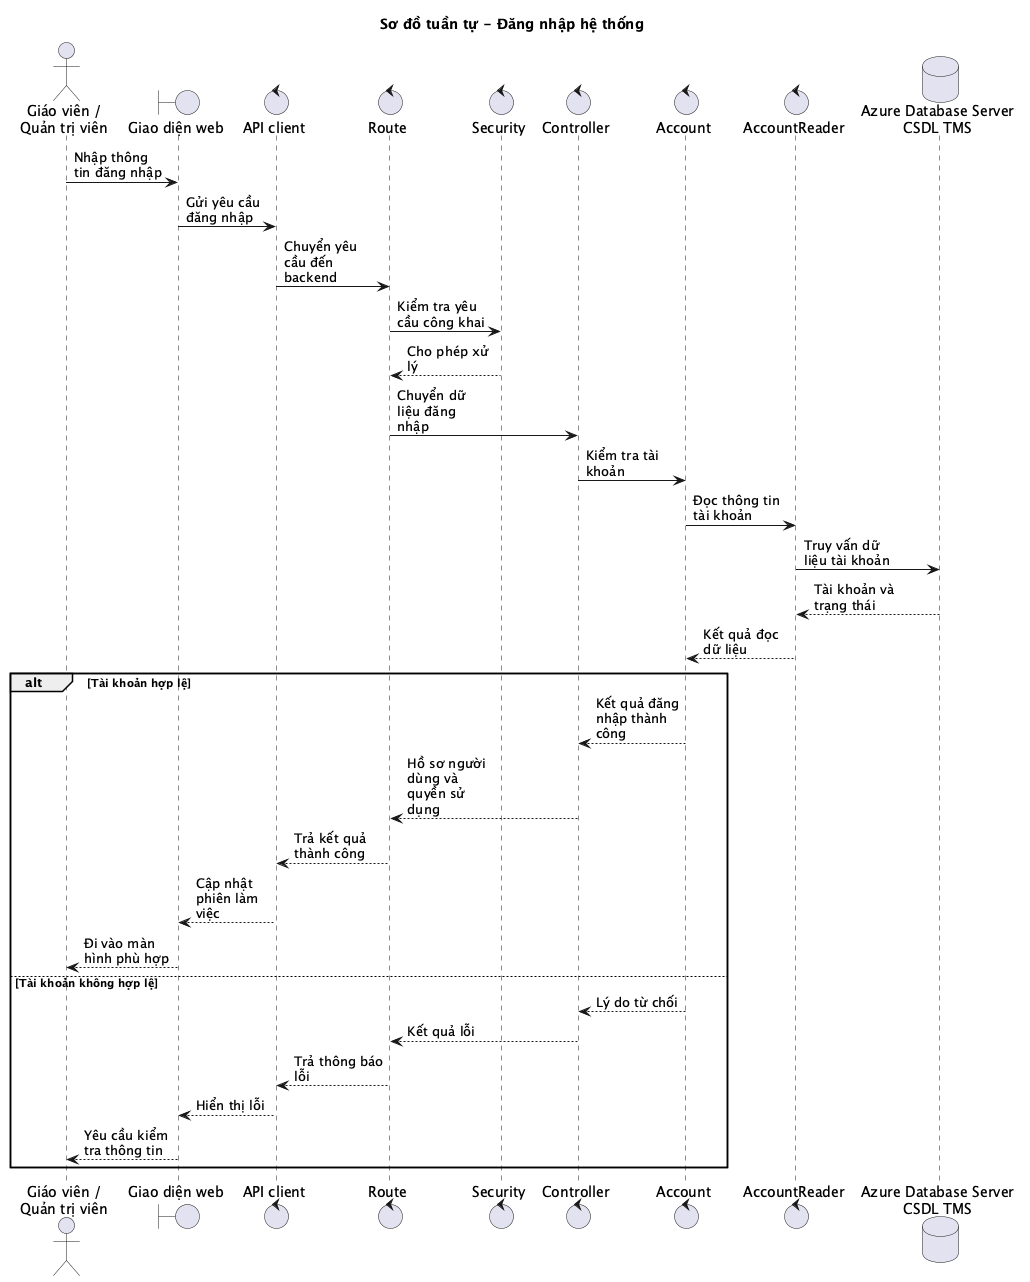
\includegraphics[width=0.96\textwidth,height=0.70\textheight,keepaspectratio]{diagrams/sequence-dang-nhap.png}
\caption{Sequence Diagram cho use case đăng nhập hệ thống}
\end{figure}

\clearpage

\subsubsection{Sequence Diagram cho worker đồng bộ thông tin từ Codeforces}

Luồng này không có actor người dùng. \code{Background Sync Worker} được
\code{SyncLoop} kích hoạt theo chu kỳ, lấy danh sách giáo viên, kiểm tra
credential Codeforces của từng giáo viên, đồng bộ catalog Gym do giáo viên sở
hữu, rồi đồng bộ standing cho các Gym đã gắn với lớp.

\begin{figure}[H]
\centering
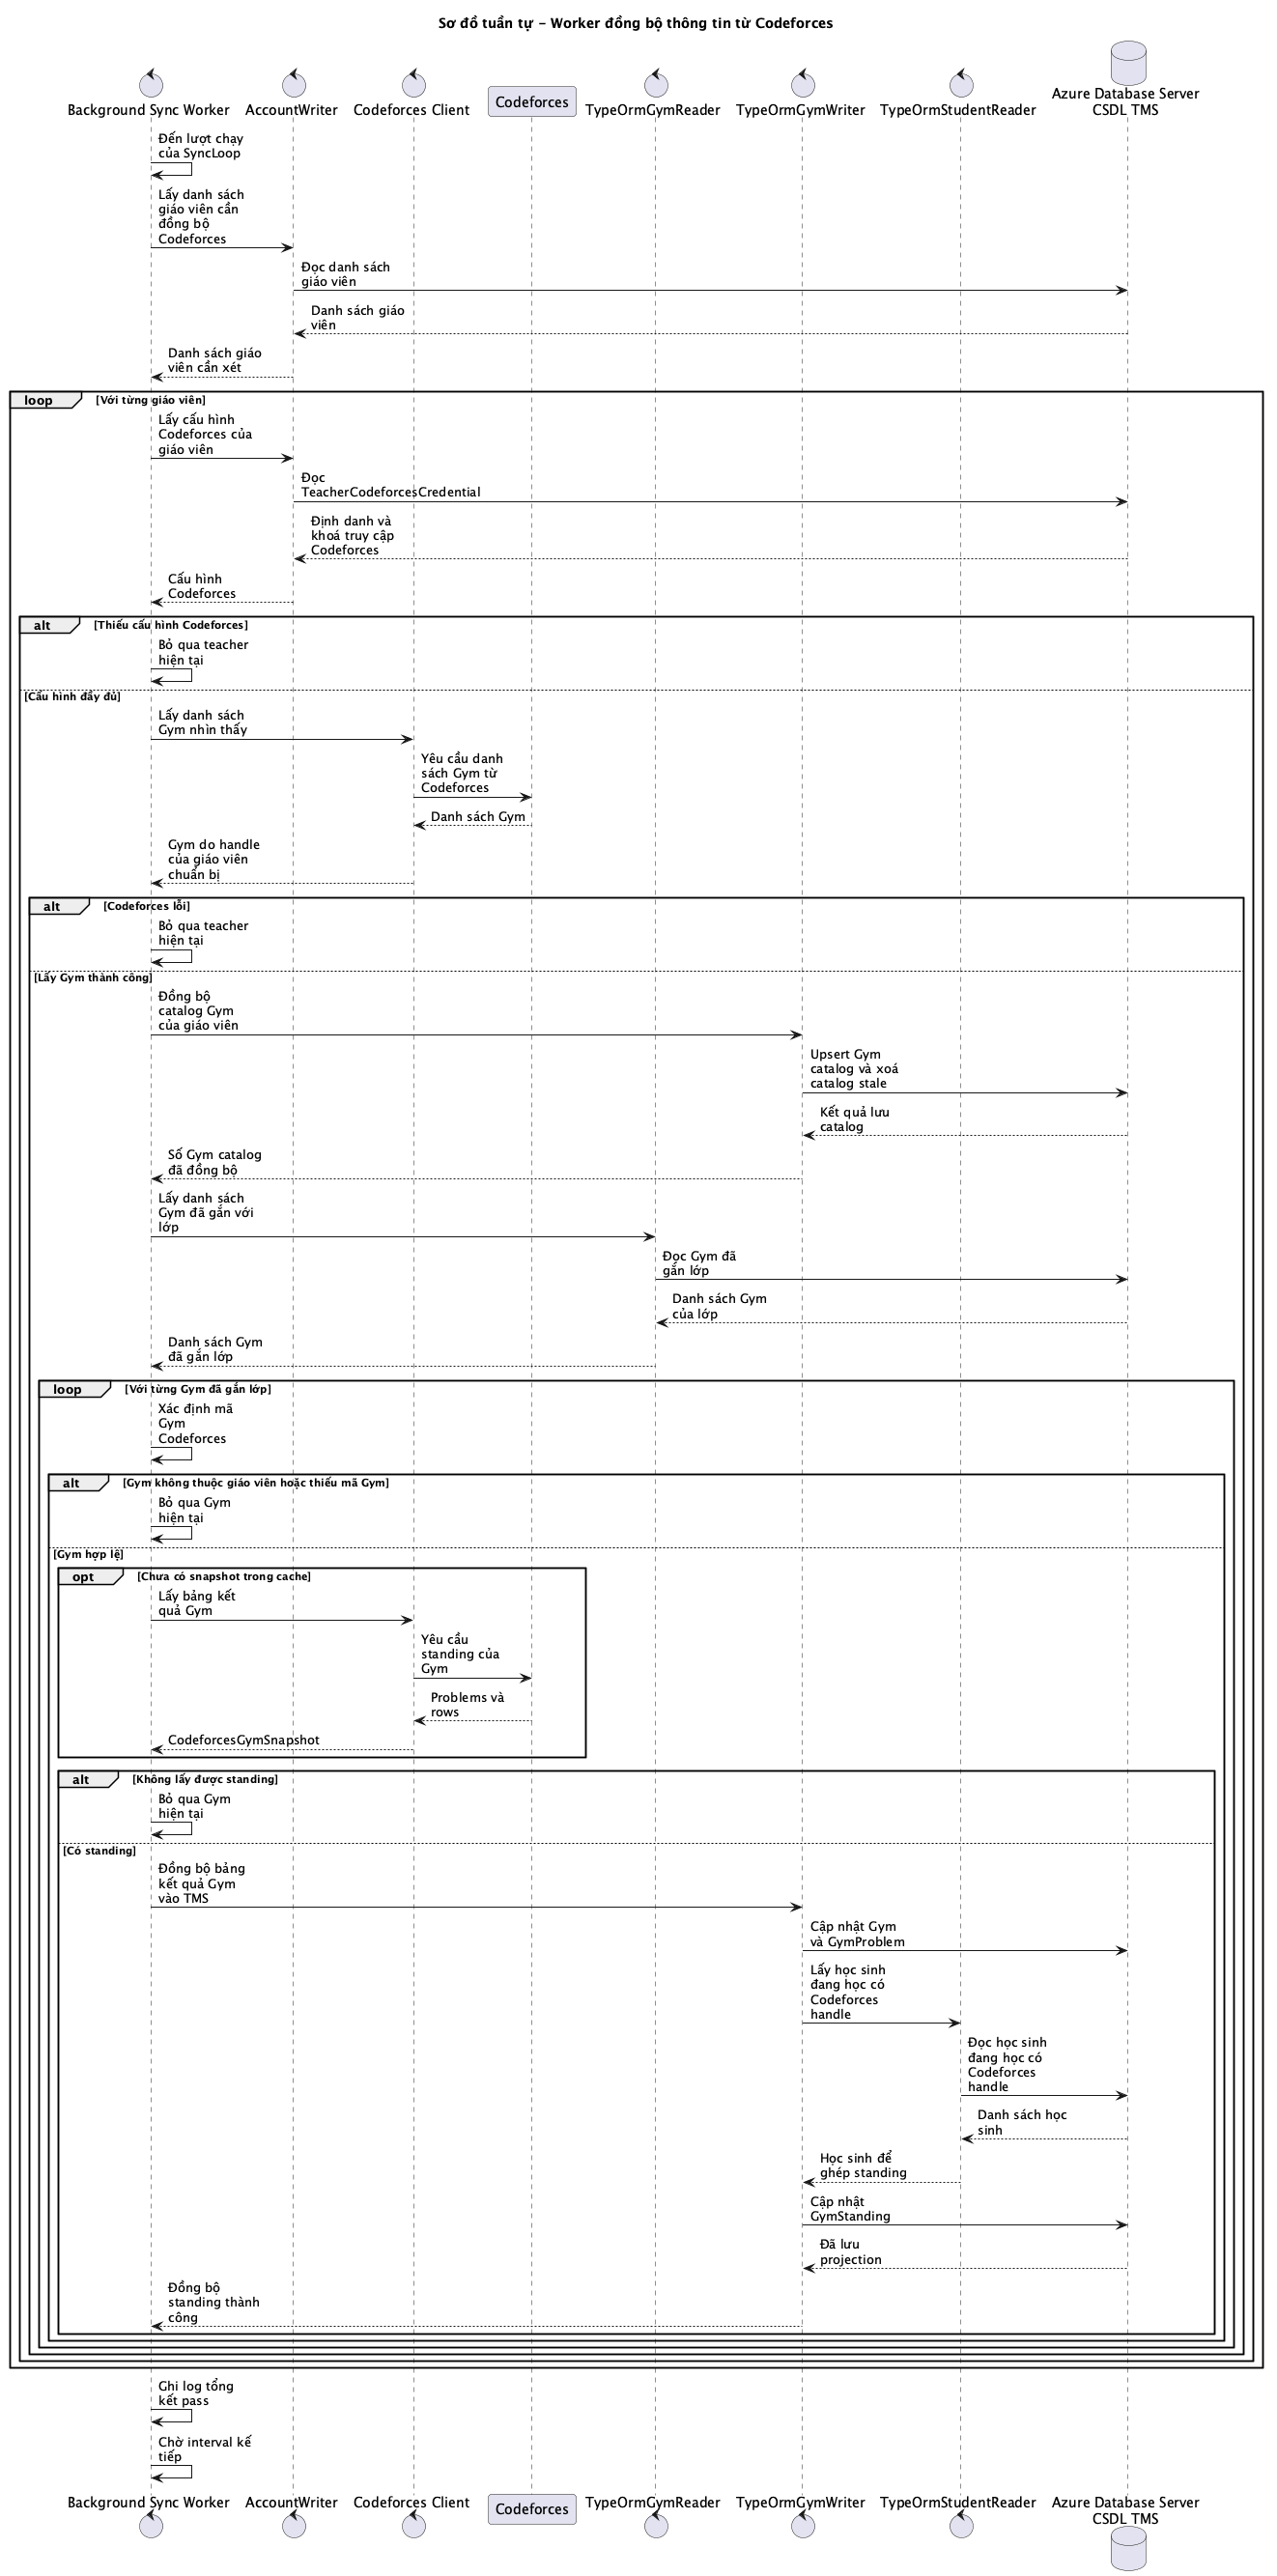
\includegraphics[width=0.96\textwidth,height=0.72\textheight,keepaspectratio]{diagrams/sequence-dong-bo-codeforces-worker.png}
\caption{Sequence Diagram cho worker đồng bộ thông tin từ Codeforces}
\end{figure}

\clearpage

\subsubsection{Sequence Diagram cho điểm danh buổi học}

Use case này đại diện cho nhóm nghiệp vụ vận hành lớp học vì sau khi giáo viên
cập nhật điểm danh, hệ thống phải kiểm tra dữ liệu lớp học, học sinh và đồng bộ
ảnh hưởng tài chính.

\begin{figure}[H]
\centering
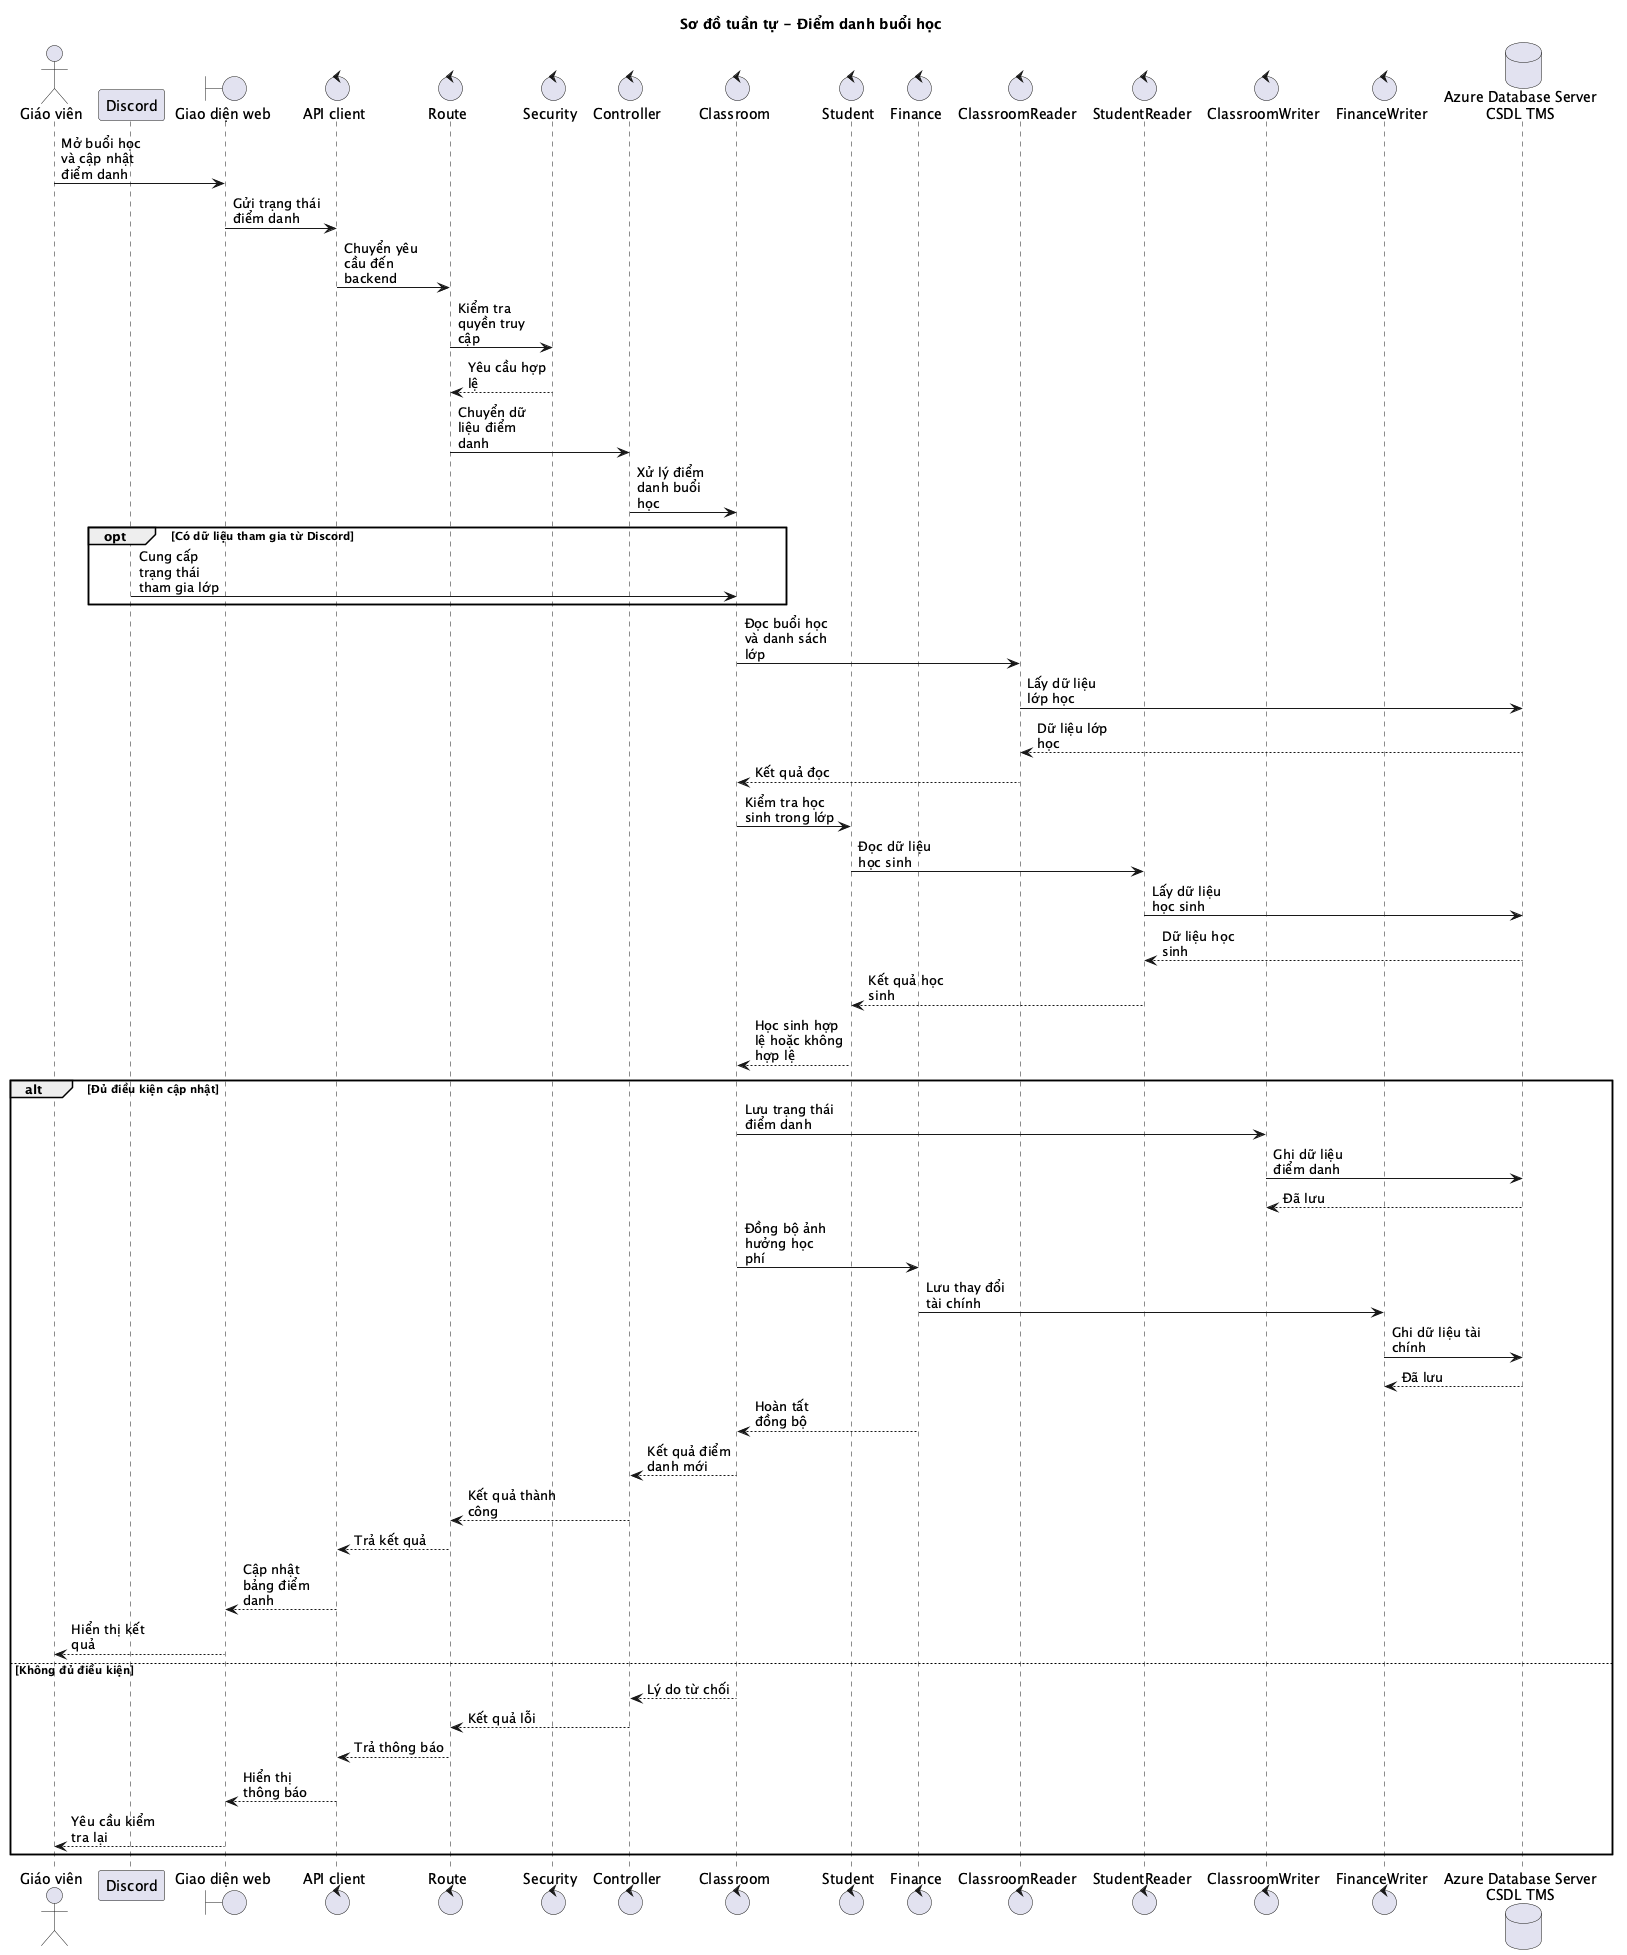
\includegraphics[width=0.96\textwidth,height=0.72\textheight,keepaspectratio]{diagrams/sequence-diem-danh-tai-chinh.png}
\caption{Sequence Diagram cho use case điểm danh buổi học}
\end{figure}

\clearpage

\subsubsection{Sequence Diagram cho uỷ quyền quản lý Discord Guild}

Use case này đại diện cho actor học sinh vì luồng xử lý đi qua hệ thống ngoài
Discord và lưu kết quả liên kết vào dữ liệu TMS.

\begin{figure}[H]
\centering
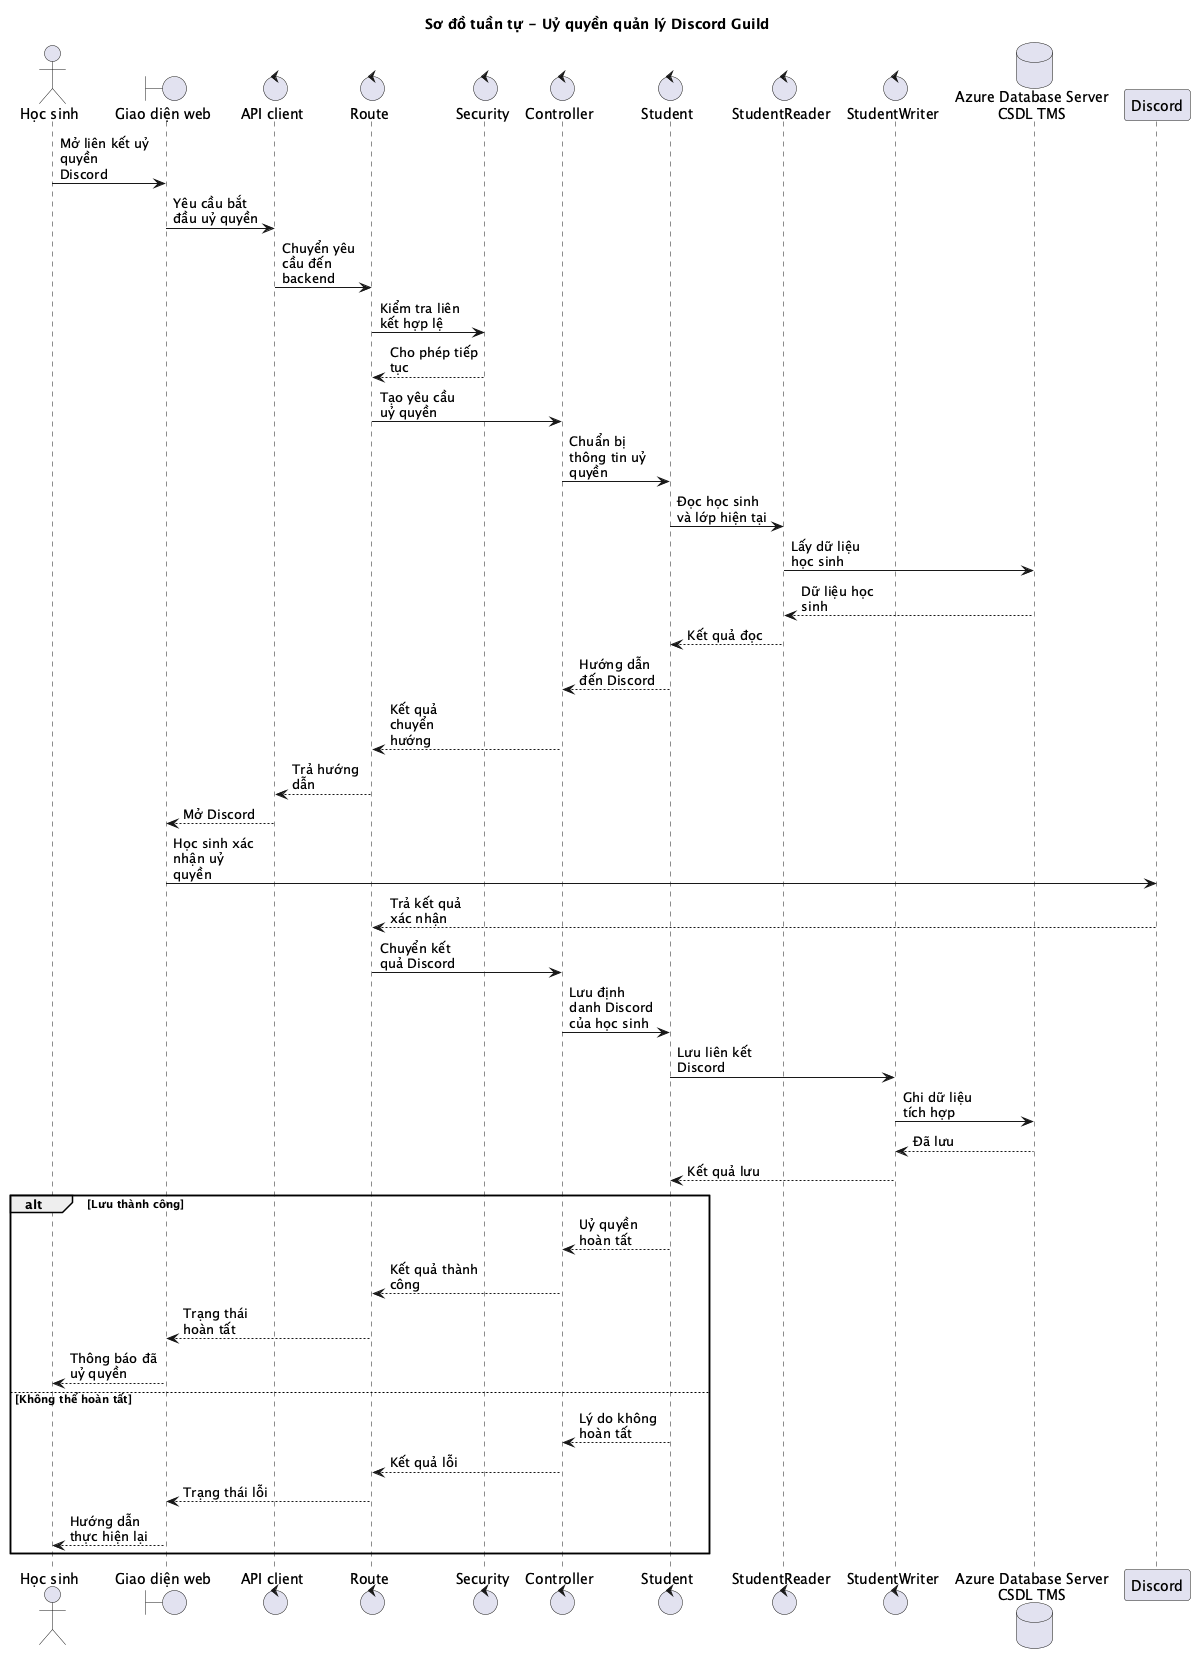
\includegraphics[width=0.96\textwidth,height=0.72\textheight,keepaspectratio]{diagrams/sequence-hoc-sinh-uy-quyen-discord.png}
\caption{Sequence Diagram cho use case uỷ quyền quản lý Discord Guild}
\end{figure}

\clearpage

\subsubsection{Sequence Diagram cho gắn Gym Codeforces cho lớp học}

Use case này thể hiện thứ tự từ lúc giáo viên chọn Gym đến khi Classroom kiểm
tra lớp học, lấy dữ liệu luyện tập khi cần và lưu liên kết Gym của lớp.

\begin{figure}[H]
\centering
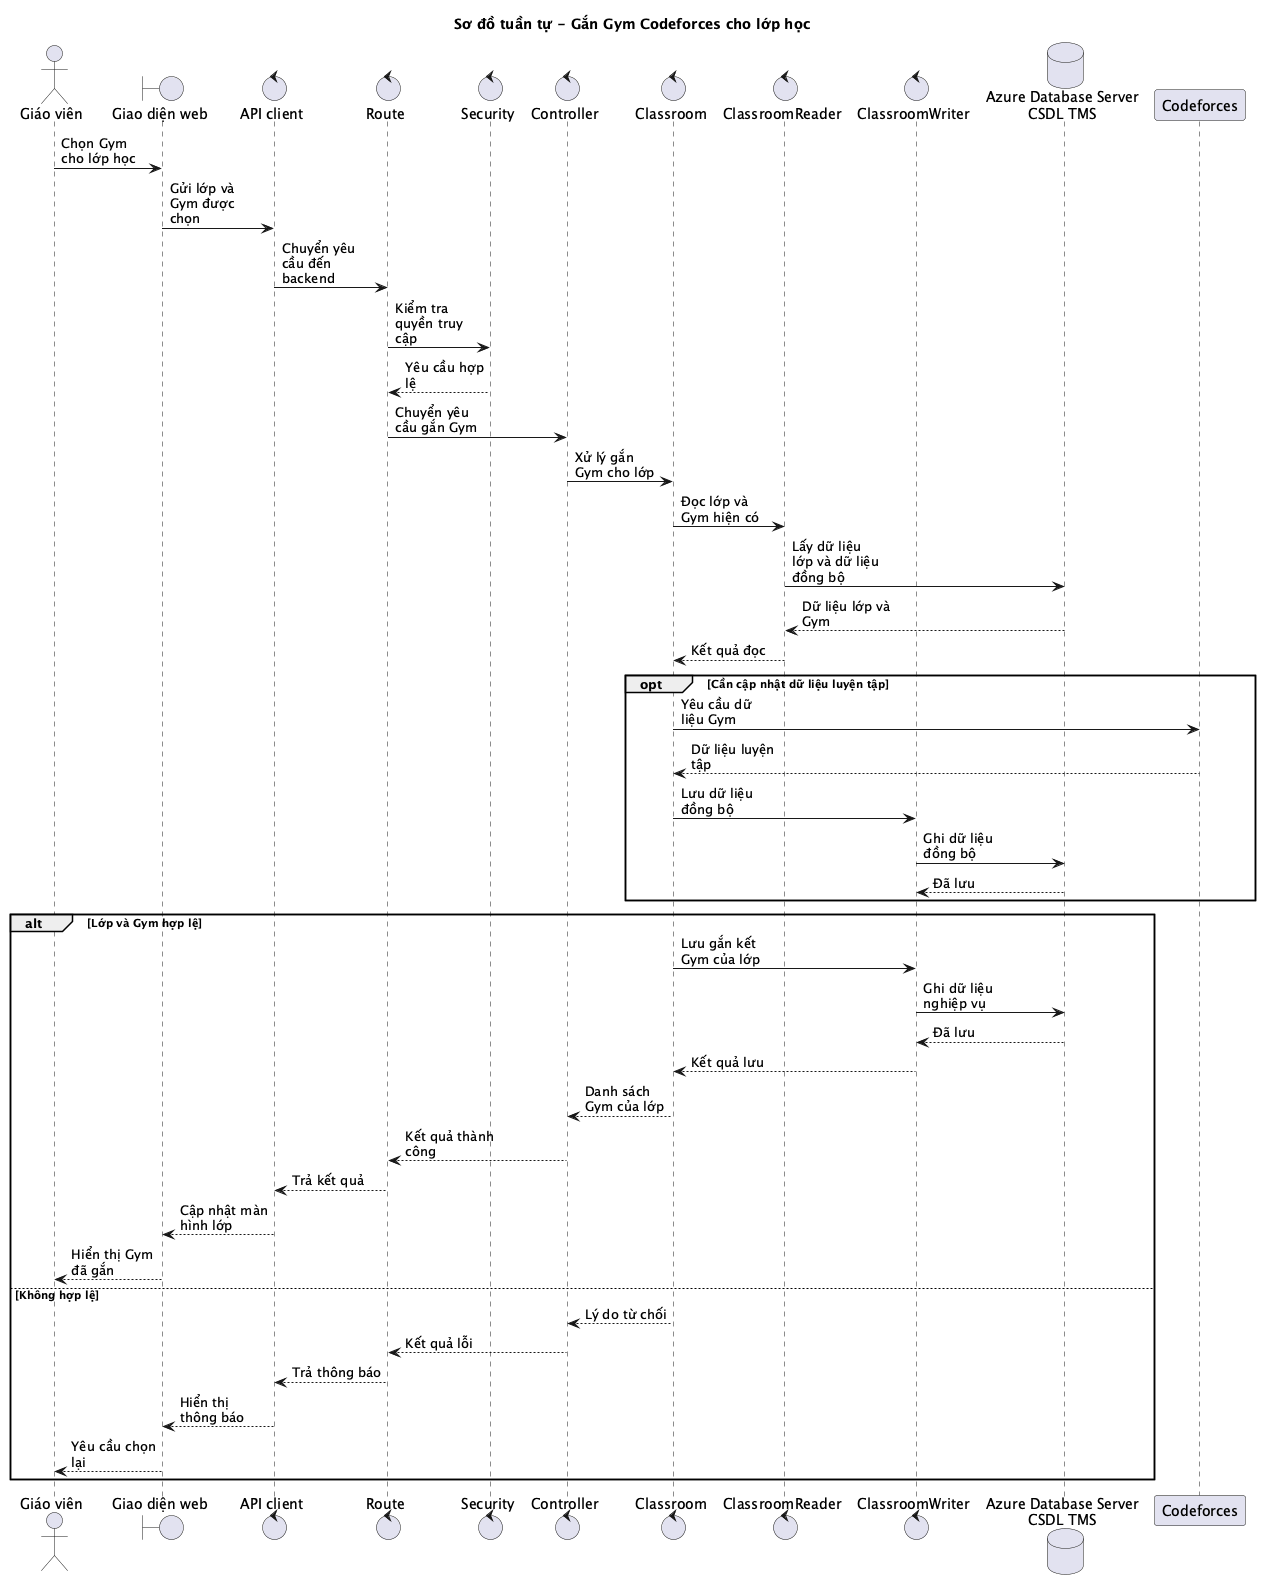
\includegraphics[width=0.96\textwidth,height=0.72\textheight,keepaspectratio]{diagrams/sequence-gan-gym-codeforces.png}
\caption{Sequence Diagram cho use case gắn Gym Codeforces cho lớp học}
\end{figure}

\clearpage

\iffalse
\subsection{Sơ đồ giao tiếp (Communication Diagram)}

Communication diagram được dùng cho các use case cần thấy rõ sự phối hợp giữa
các thành phần trong kiến trúc. Các object trong sơ đồ giữ đúng tên thành phần
kiến trúc, không đưa thêm object nghiệp vụ chi tiết.

\begin{table}[!htbp]
\centering
\tablesetup
\begin{tabularx}{\textwidth}{|C{1.0cm}|L{4.0cm}|Y|}
\hline
\textbf{STT} & \textbf{Use case tiêu biểu} & \textbf{Lý do chọn} \\
\hline
1 & Worker đồng bộ thông tin từ Codeforces & Thể hiện quan hệ phối hợp giữa Background Sync Worker, AccountWriter, Codeforces Client, TypeOrmGymReader, TypeOrmGymWriter và TypeOrmStudentReader. \\
\hline
2 & Điểm danh buổi học & Thể hiện sự phối hợp giữa Classroom, Student, Finance và Discord. \\
\hline
3 & Thiết lập Discord cho lớp học & Thể hiện quan hệ giữa Account, Classroom, Discord và dữ liệu lưu trữ. \\
\hline
4 & Gửi thông báo cho học sinh & Thể hiện cách Classroom và Student cùng cung cấp dữ liệu nhận tin cho Discord. \\
\hline
5 & Quản lý giao dịch tài chính & Thể hiện sự phối hợp giữa Finance và Student trước khi lưu dữ liệu tài chính. \\
\hline
\end{tabularx}
\end{table}

\subsubsection{Communication Diagram cho worker đồng bộ thông tin từ Codeforces}

\begin{figure}[H]
\centering
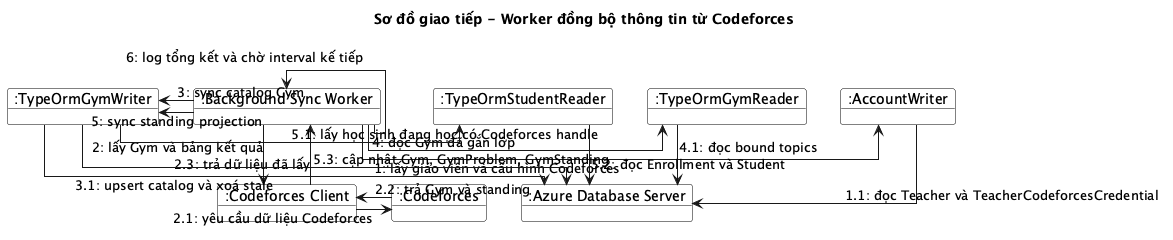
\includegraphics[width=0.96\textwidth,height=0.72\textheight,keepaspectratio]{diagrams/communication-dong-bo-codeforces-worker.png}
\caption{Communication Diagram cho worker đồng bộ thông tin từ Codeforces}
\end{figure}

\clearpage

\subsubsection{Communication Diagram cho điểm danh buổi học}

\begin{figure}[H]
\centering
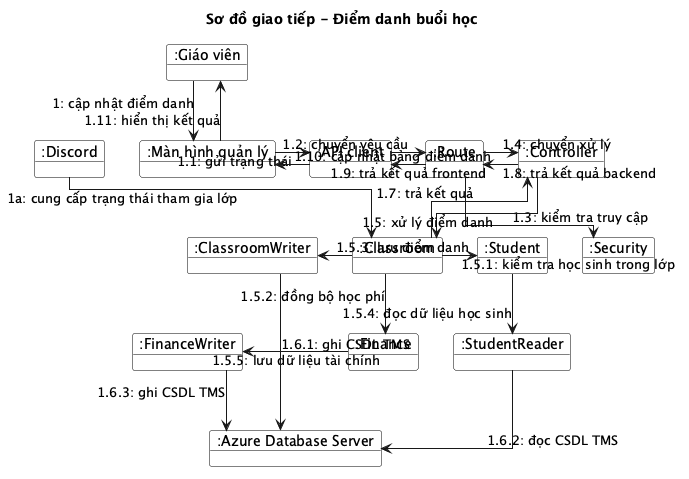
\includegraphics[width=0.96\textwidth,height=0.72\textheight,keepaspectratio]{diagrams/communication-diem-danh-buoi-hoc.png}
\caption{Communication Diagram cho use case điểm danh buổi học}
\end{figure}

\clearpage

\subsubsection{Communication Diagram cho thiết lập Discord cho lớp học}

\begin{figure}[H]
\centering
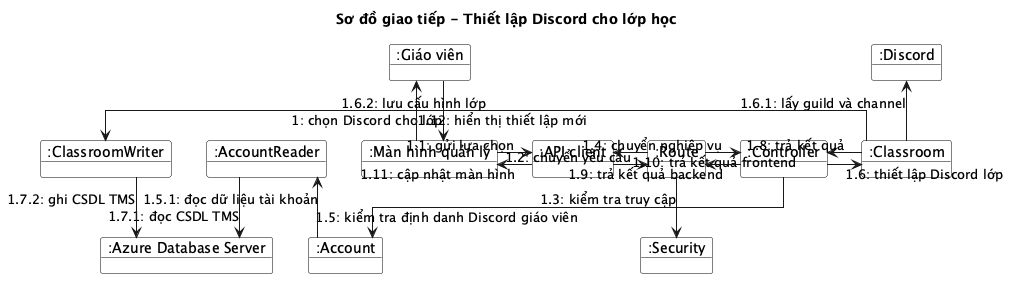
\includegraphics[width=0.96\textwidth,height=0.72\textheight,keepaspectratio]{diagrams/communication-thiet-lap-discord-lop.png}
\caption{Communication Diagram cho use case thiết lập Discord cho lớp học}
\end{figure}

\clearpage

\subsubsection{Communication Diagram cho gửi thông báo cho học sinh}

\begin{figure}[H]
\centering
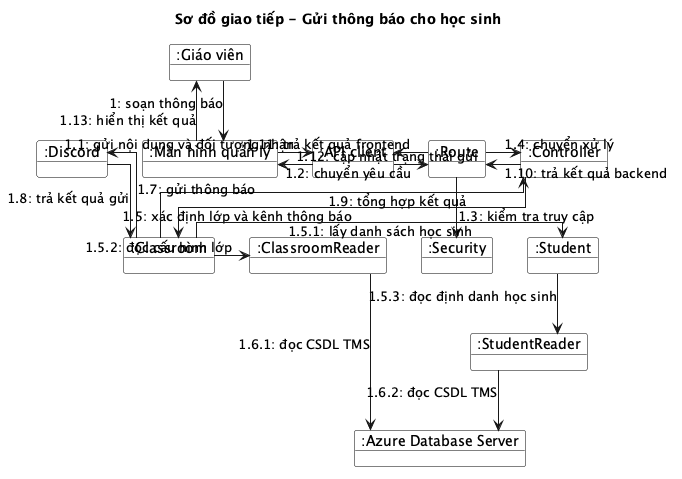
\includegraphics[width=0.96\textwidth,height=0.72\textheight,keepaspectratio]{diagrams/communication-gui-thong-bao.png}
\caption{Communication Diagram cho use case gửi thông báo cho học sinh}
\end{figure}

\clearpage

\subsubsection{Communication Diagram cho quản lý giao dịch tài chính}

\begin{figure}[H]
\centering
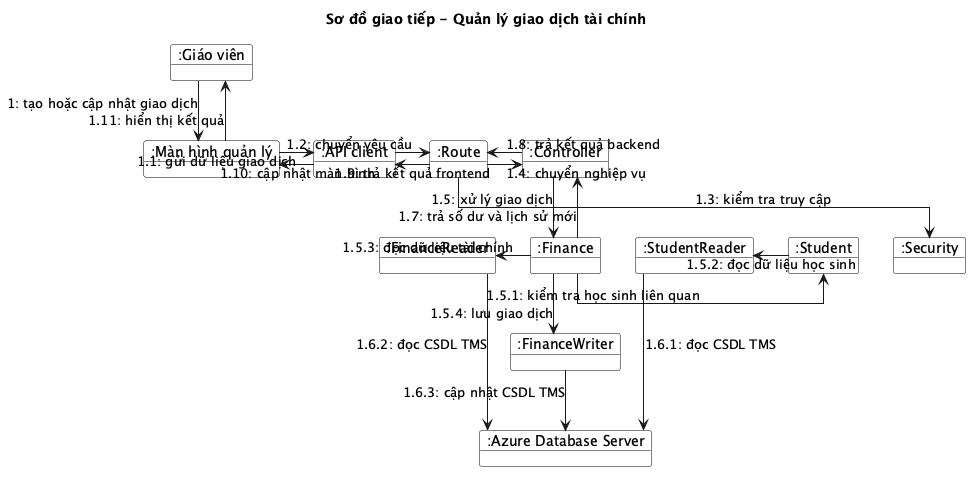
\includegraphics[width=0.96\textwidth,height=0.72\textheight,keepaspectratio]{diagrams/communication-quan-ly-giao-dich.png}
\caption{Communication Diagram cho use case quản lý giao dịch tài chính}
\end{figure}

\clearpage

\fi

\subsection{Sơ đồ hoạt động (Activity Diagram)}

Activity diagram được dùng để mô tả luồng hoạt động của một quy trình nghiệp vụ hoặc use case.
Các sơ đồ trong phần này tập trung vào thứ tự công việc, decision/branching và kết quả nghiệp vụ tiếp theo; không mô tả object, class, function call hay các tầng kỹ thuật triển khai.

\begin{table}[!htbp]
\centering
\tablesetup
\begin{tabularx}{\textwidth}{|C{1.0cm}|L{4.0cm}|Y|}
\hline
\textbf{STT} & \textbf{Use case tiêu biểu} & \textbf{Lý do chọn} \\
\hline
1 & Quản lý học sinh & Có các nhánh tạo mới, cập nhật và tra cứu. \\
\hline
2 & Worker đồng bộ thông tin từ Codeforces & Có vòng lặp theo từng giáo viên, từng Gym đã gắn lớp và các nhánh bỏ qua khi thiếu credential, lỗi Codeforces hoặc Gym không hợp lệ. \\
\hline
3 & Quản lý buổi học & Có nhánh xem danh sách, tạo buổi học và hủy buổi học. \\
\hline
4 & Điểm danh buổi học & Có kiểm tra buổi học, học sinh và đồng bộ tài chính. \\
\hline
5 & Xử lý học sinh chờ lưu trữ & Có quyết định rõ theo trạng thái tài chính đã hoàn tất hay chưa. \\
\hline
\end{tabularx}
\end{table}

\subsubsection{Activity Diagram cho quản lý học sinh}

\begin{figure}[H]
\centering
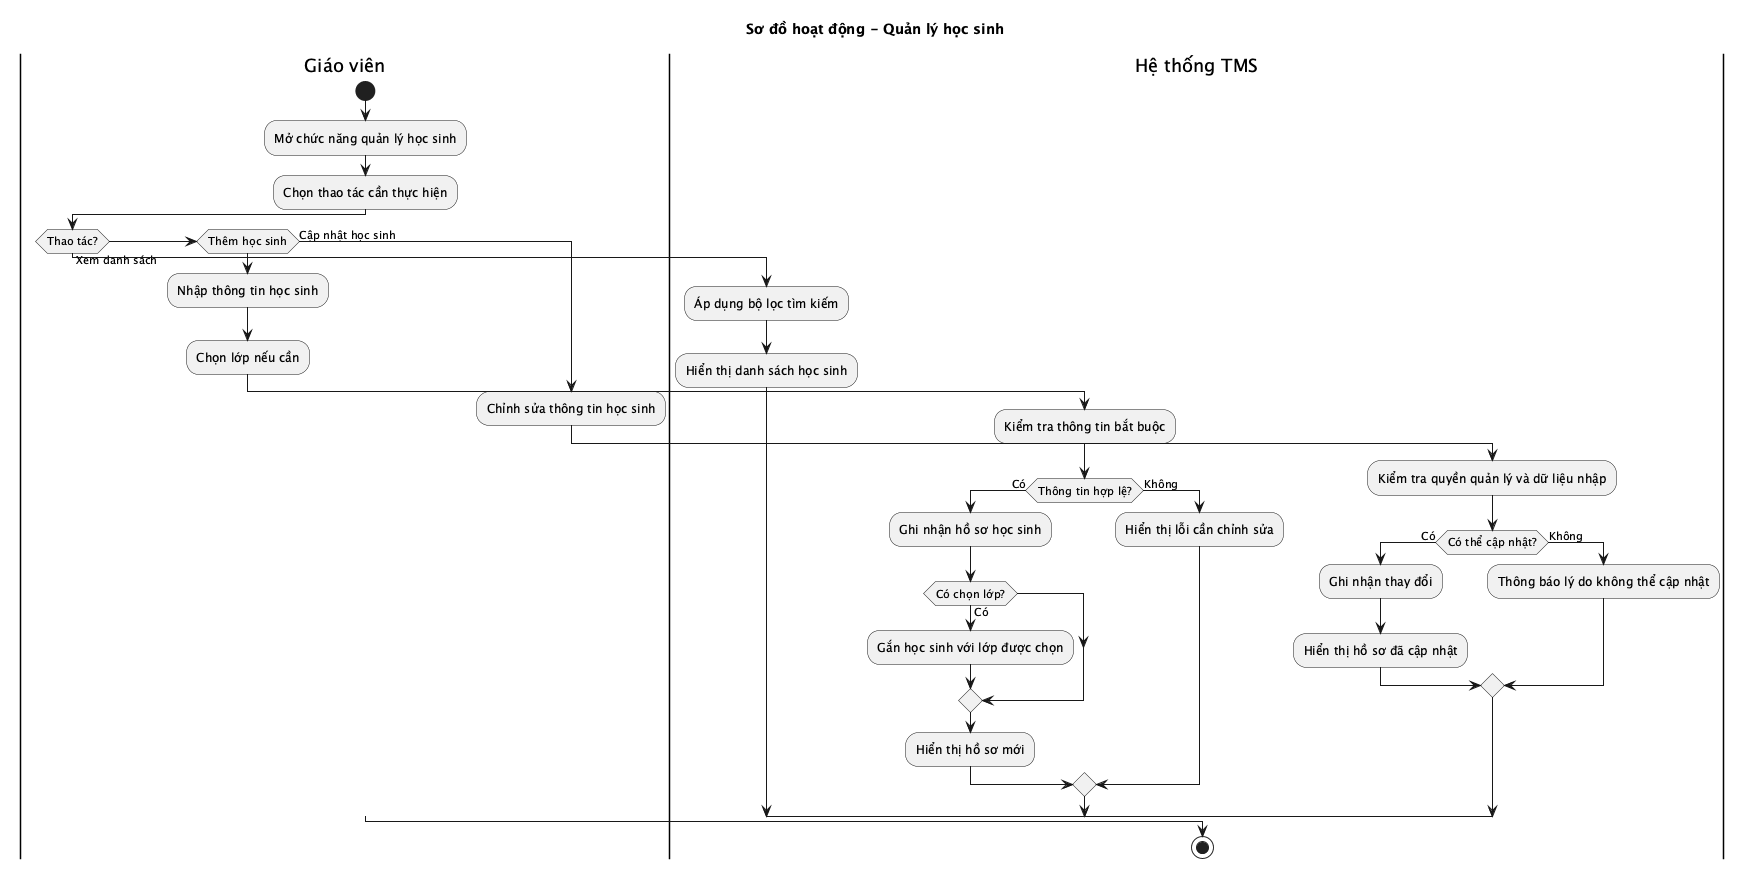
\includegraphics[width=0.96\textwidth,height=0.72\textheight,keepaspectratio]{diagrams/activity-quan-ly-hoc-sinh.png}
\caption{Activity Diagram cho use case quản lý học sinh}
\end{figure}

\clearpage

\subsubsection{Activity Diagram cho worker đồng bộ thông tin từ Codeforces}

\begin{figure}[H]
\centering
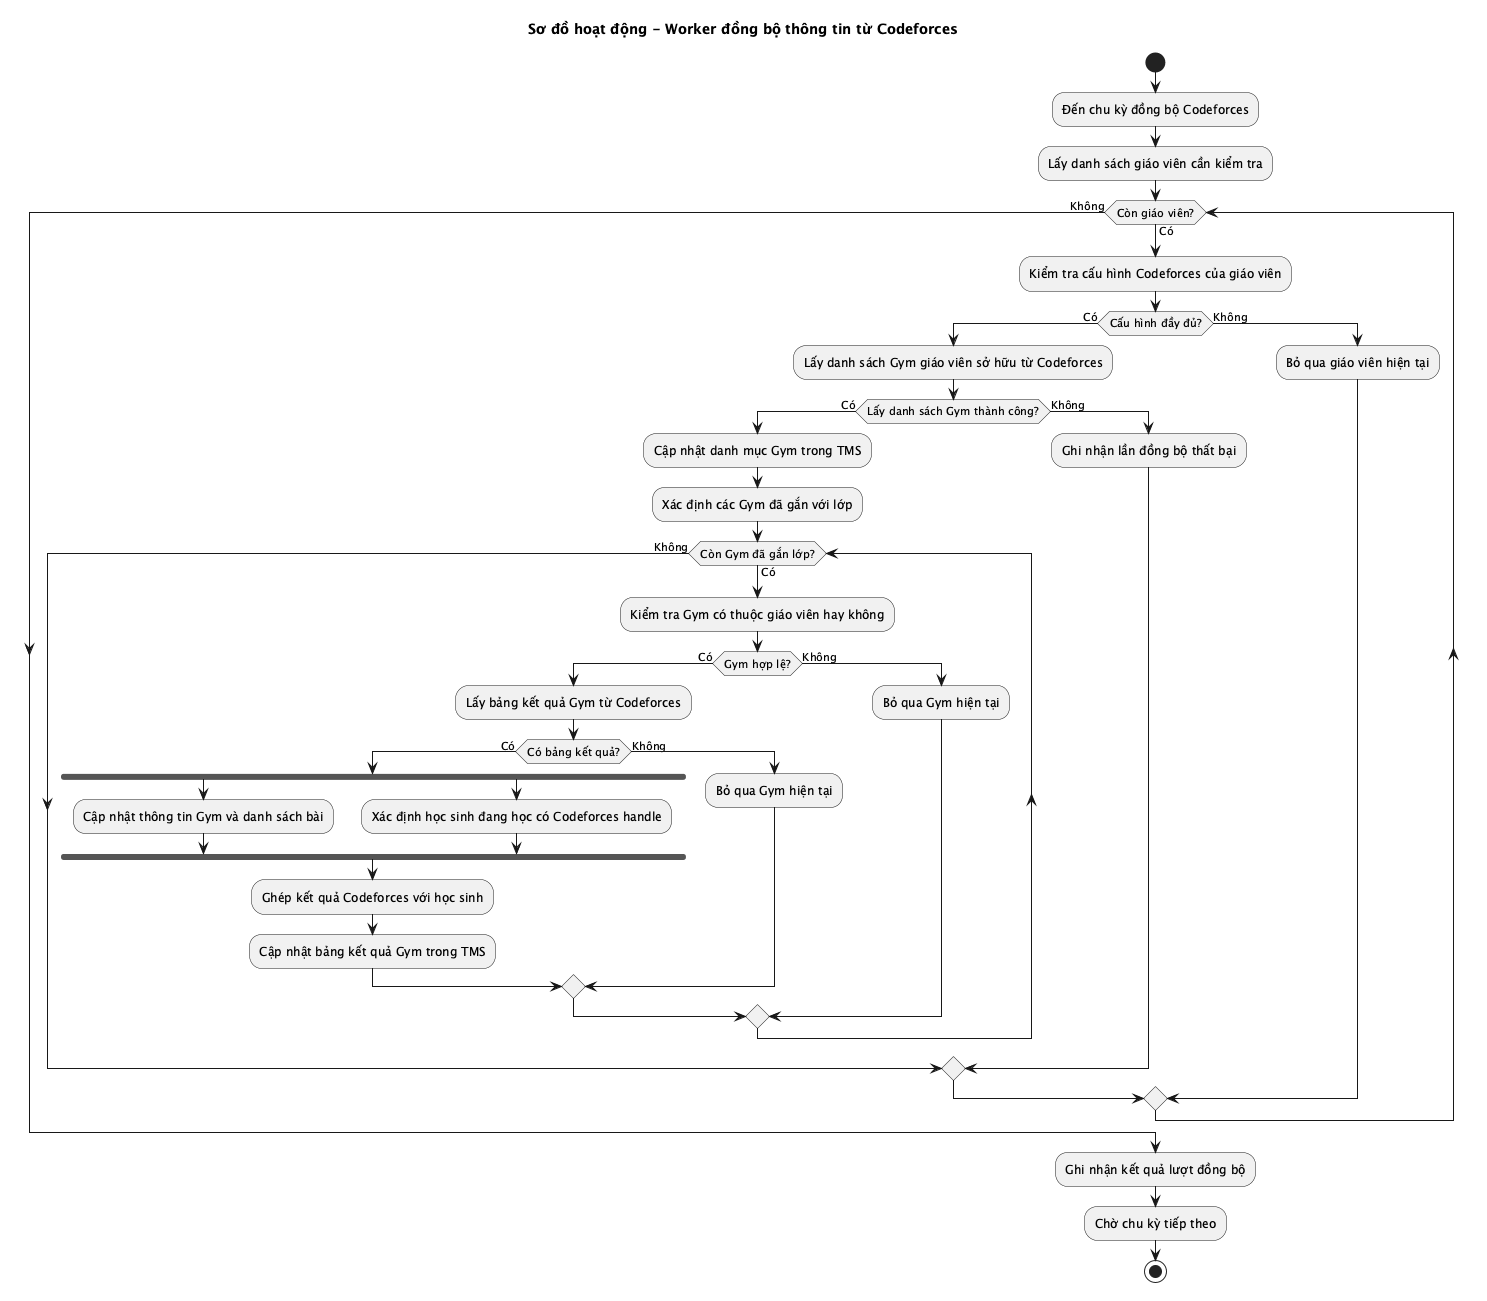
\includegraphics[width=0.96\textwidth,height=0.72\textheight,keepaspectratio]{diagrams/activity-dong-bo-codeforces-worker.png}
\caption{Activity Diagram cho worker đồng bộ thông tin từ Codeforces}
\end{figure}

\clearpage

\subsubsection{Activity Diagram cho quản lý buổi học}

\begin{figure}[H]
\centering
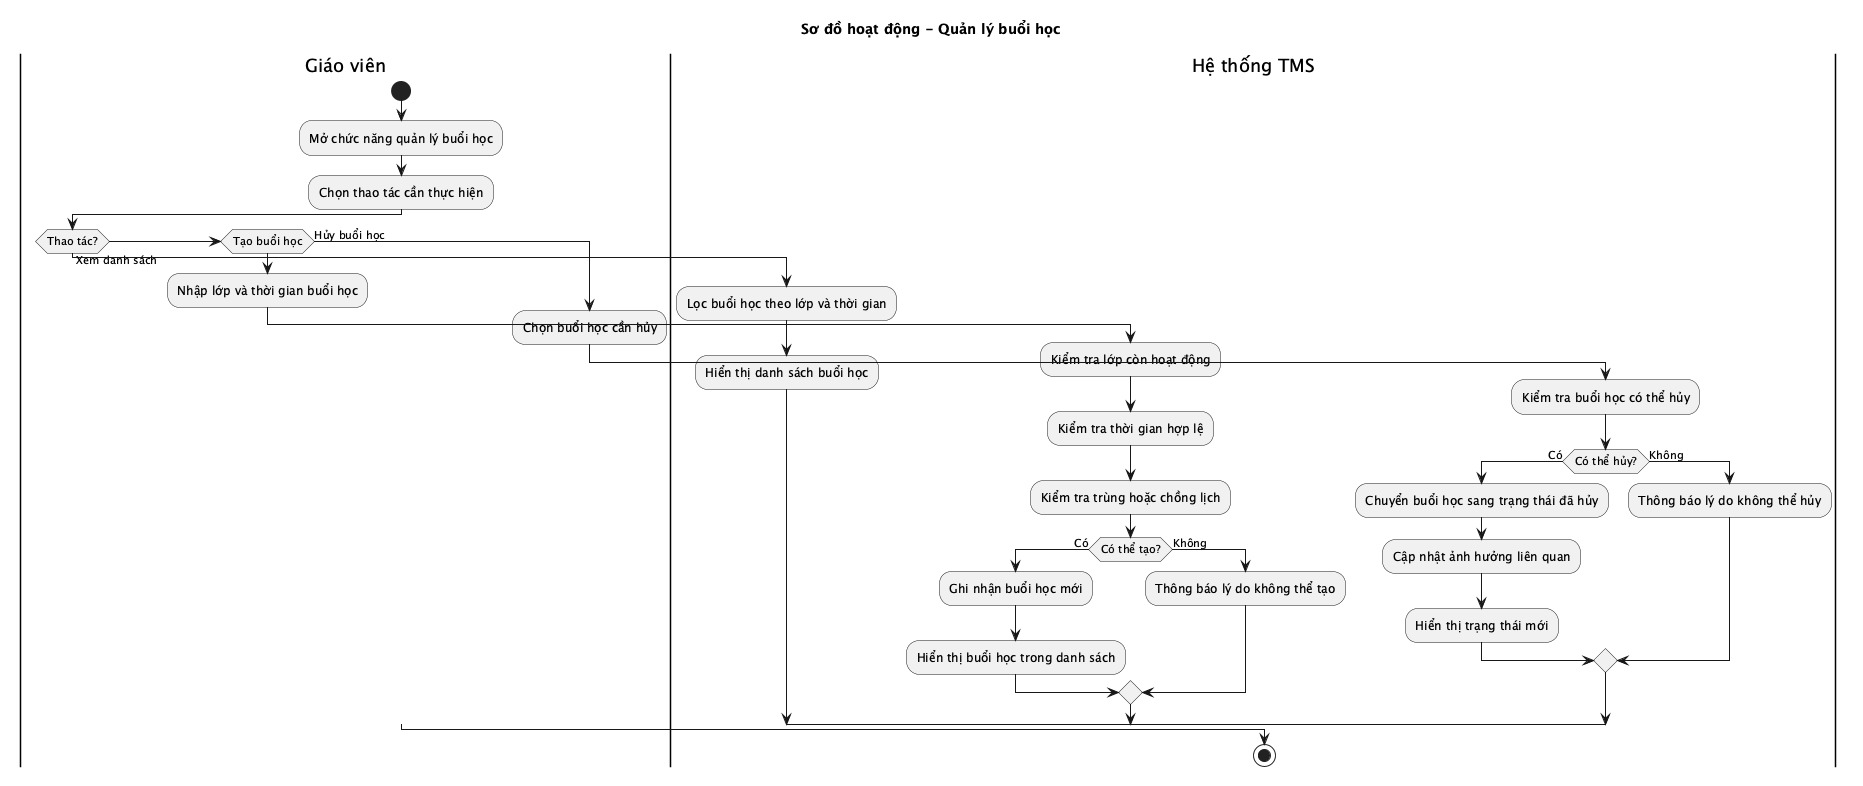
\includegraphics[width=0.96\textwidth,height=0.72\textheight,keepaspectratio]{diagrams/activity-quan-ly-buoi-hoc.png}
\caption{Activity Diagram cho use case quản lý buổi học}
\end{figure}

\clearpage

\subsubsection{Activity Diagram cho điểm danh buổi học}

\begin{figure}[H]
\centering
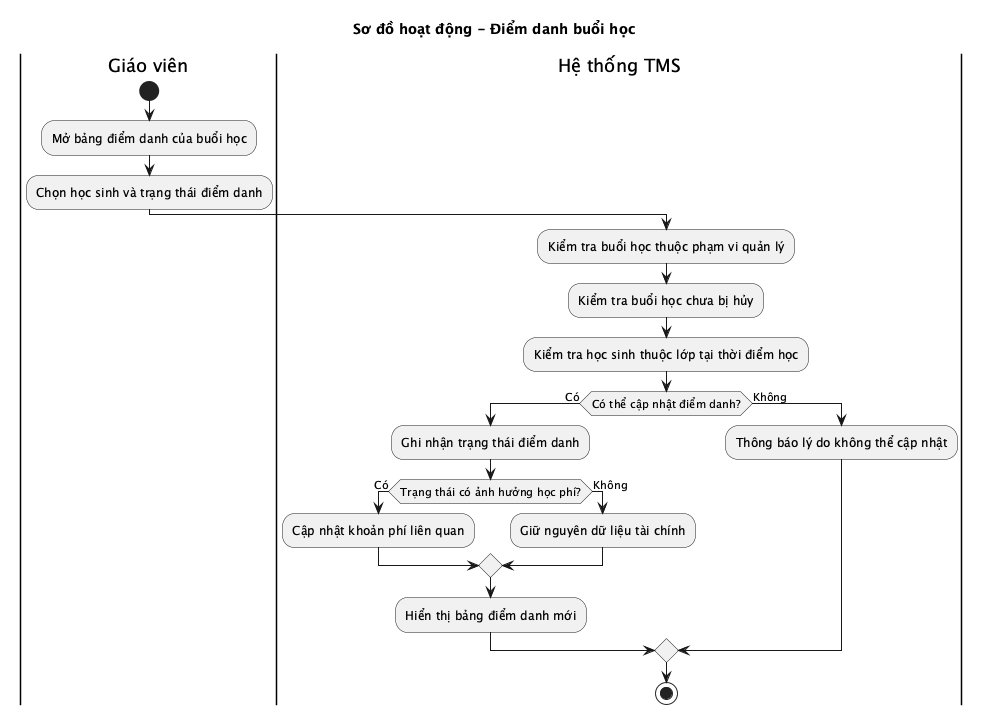
\includegraphics[width=0.96\textwidth,height=0.72\textheight,keepaspectratio]{diagrams/activity-diem-danh-buoi-hoc.png}
\caption{Activity Diagram cho use case điểm danh buổi học}
\end{figure}

\clearpage

\subsubsection{Activity Diagram cho xử lý học sinh chờ lưu trữ}

\begin{figure}[H]
\centering
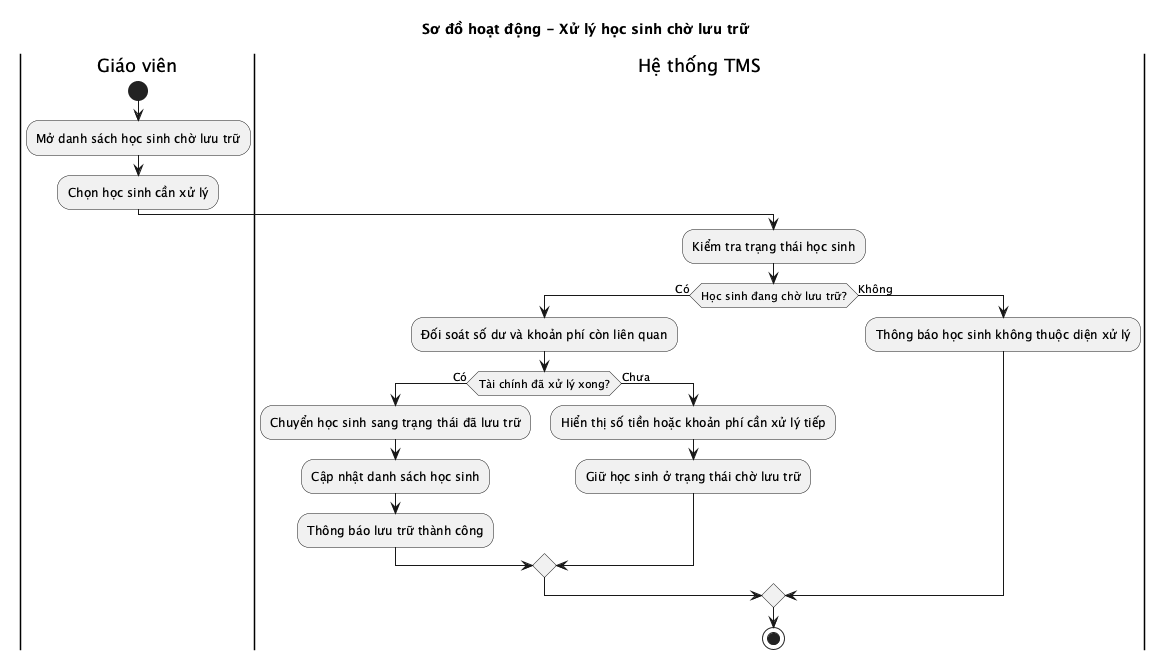
\includegraphics[width=0.96\textwidth,height=0.72\textheight,keepaspectratio]{diagrams/activity-xu-ly-cho-luu-tru.png}
\caption{Activity Diagram cho use case xử lý học sinh chờ lưu trữ}
\end{figure}

\clearpage

\setcounter{section}{4}
\section{Kiến trúc hệ thống}

Phần này trình bày kiến trúc tổng thể của hệ thống Tutor Management System
(TMS) ở mức thiết kế hệ thống. Nội dung tập trung vào các thành phần chính,
cách bố trí các thành phần và quan hệ phụ thuộc giữa chúng. Các luồng nghiệp vụ
chi tiết không được lặp lại trong phần này vì đã được mô hình hóa ở phần yêu
cầu chức năng.

\subsection{Mô hình kiến trúc}

TMS sử dụng mô hình client--server: trình duyệt gửi request đến backend, backend
xử lý nghiệp vụ và lưu dữ liệu trên Azure Database Server.

Ở mức triển khai backend, hệ thống chọn kiến trúc modular monolith. Backend vẫn
là một ứng dụng duy nhất, nhưng được chia theo các ranh giới nghiệp vụ bên
trong. Cách này đủ rõ ràng cho phạm vi đồ án và tránh độ phức tạp của nhiều
dịch vụ độc lập.

\subsection{Sơ đồ kiến trúc}

\begin{figure}[H]
    \centering
    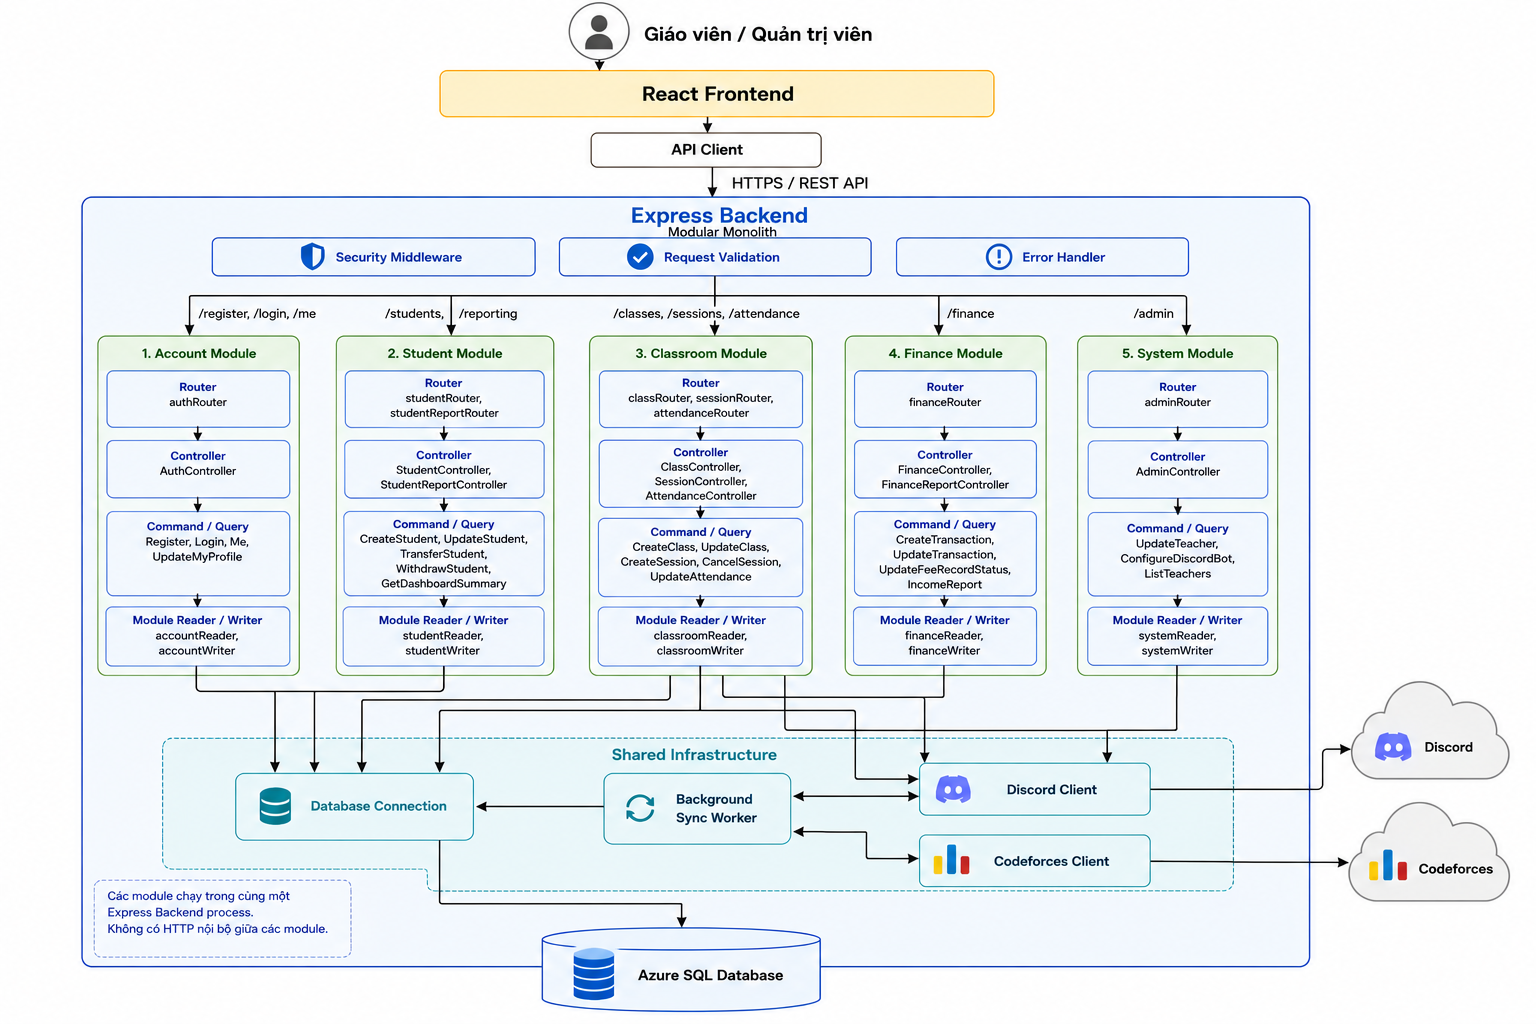
\includegraphics[width=0.98\textwidth,height=0.72\textheight,keepaspectratio]{diagrams/tong-the-kien-truc.png}
    \caption{Sơ đồ kiến trúc hệ thống TMS}
\end{figure}

\subsection{Mô tả các thành phần trong hệ thống}

\begingroup
\singlespacing
\setlength{\parskip}{0pt}
\renewcommand{\arraystretch}{1.25}
\footnotesize
\begin{longtable}{|p{1.2cm}|p{4.2cm}|p{9.0cm}|}
\hline
\textbf{STT} & \textbf{Thành phần} & \textbf{Mô tả} \\
\hline
\endhead
1 & Giáo viên / Quản trị viên & Người sử dụng hệ thống thông qua giao diện web. Giáo viên thao tác với dữ liệu lớp học, học sinh, điểm danh và tài chính; quản trị viên quản lý tài khoản và cấu hình hệ thống. \\
\hline
2 & React Frontend & Giao diện người dùng chạy trên trình duyệt, cung cấp các màn hình thao tác cho giáo viên và quản trị viên. \\
\hline
3 & API Client & Lớp phía frontend chịu trách nhiệm gửi request đến backend thông qua REST API. \\
\hline
4 & Express Backend & Ứng dụng backend chính của hệ thống. Backend chạy theo mô hình modular monolith, tiếp nhận request từ frontend và điều phối xử lý nghiệp vụ. \\
\hline
5 & Security Middleware & Lớp kiểm soát truy cập trước khi request đi vào module nghiệp vụ, gồm xác thực và kiểm tra quyền truy cập. \\
\hline
6 & Request Validation & Lớp kiểm tra dữ liệu đầu vào của request trước khi chuyển vào controller. \\
\hline
7 & Error Handler & Lớp chuẩn hóa lỗi và response lỗi trả về cho frontend. \\
\hline
8 & Account Module & Module phụ trách đăng nhập, đăng ký, hồ sơ tài khoản và thông tin định danh liên quan đến tài khoản. \\
\hline
9 & Student Module & Module phụ trách học sinh, ghi danh, chuyển lớp, rút khỏi lớp và các truy vấn tổng quan liên quan đến học sinh. \\
\hline
10 & Classroom Module & Module phụ trách lớp học, lịch học, buổi học, điểm danh và các chức năng học tập liên quan đến lớp. \\
\hline
11 & Finance Module & Module phụ trách giao dịch, khoản phí, trạng thái phí và báo cáo tài chính. \\
\hline
12 & System Module & Module phụ trách chức năng quản trị hệ thống, gồm quản lý tài khoản giáo viên và cấu hình dùng chung. \\
\hline
13 & Database Connection & Thành phần hạ tầng dùng chung để các reader/writer của module truy cập cơ sở dữ liệu. \\
\hline
14 & Background Sync Worker & Tác vụ nền dùng để đồng bộ dữ liệu định kỳ giữa hệ thống với các dịch vụ bên ngoài và cơ sở dữ liệu. \\
\hline
15 & Discord Client & Thành phần hạ tầng dùng để backend giao tiếp với Discord. \\
\hline
16 & Codeforces Client & Thành phần hạ tầng dùng để backend giao tiếp với Codeforces. \\
\hline
17 & Azure SQL Database & Cơ sở dữ liệu chính của hệ thống, lưu dữ liệu nghiệp vụ và dữ liệu đồng bộ cần hiển thị trong TMS. \\
\hline
18 & Discord & Dịch vụ bên ngoài được tích hợp để hỗ trợ các chức năng liên quan đến lớp học và cộng đồng học viên. \\
\hline
19 & Codeforces & Dịch vụ bên ngoài được tích hợp để đồng bộ dữ liệu luyện tập, bài tập và kết quả học tập. \\
\hline
\end{longtable}
\endgroup

\subsection{Thiết kế API endpoint}

Hệ thống sử dụng REST API.

\begin{figure}[H]
    \centering
    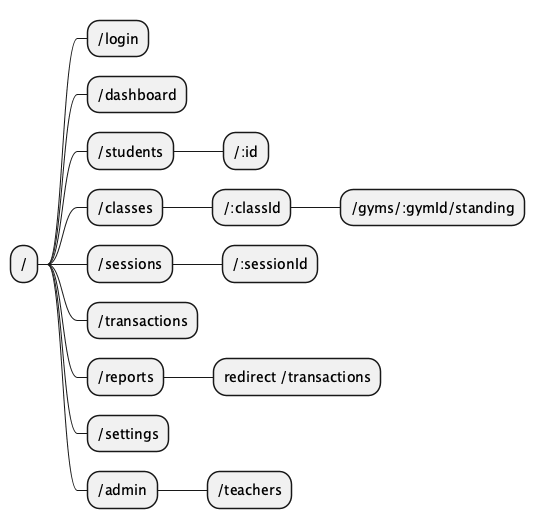
\includegraphics[width=0.96\textwidth,height=0.70\textheight,keepaspectratio]{diagrams/api-endpoint-frontend.png}
    \caption{Các endpoint giao diện hiện tại của frontend}
\end{figure}

\begin{figure}[H]
    \centering
    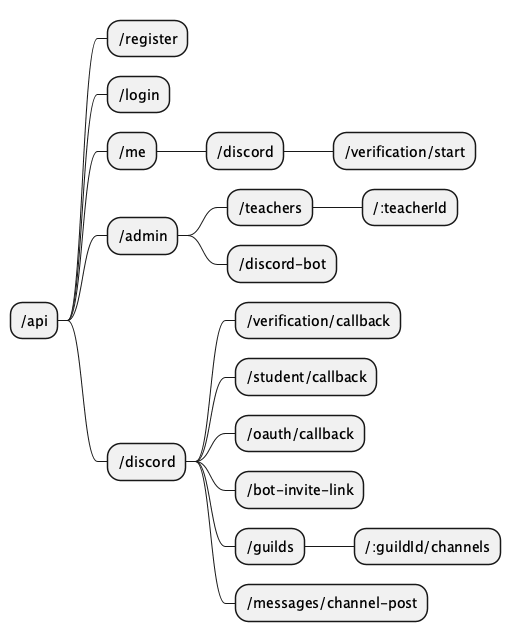
\includegraphics[width=0.96\textwidth,height=0.70\textheight,keepaspectratio]{diagrams/api-endpoint-backend-core.png}
      \caption{Các REST endpoint backend: tài khoản, quản trị và Discord}
\end{figure}

\begin{figure}[H]
    \centering
    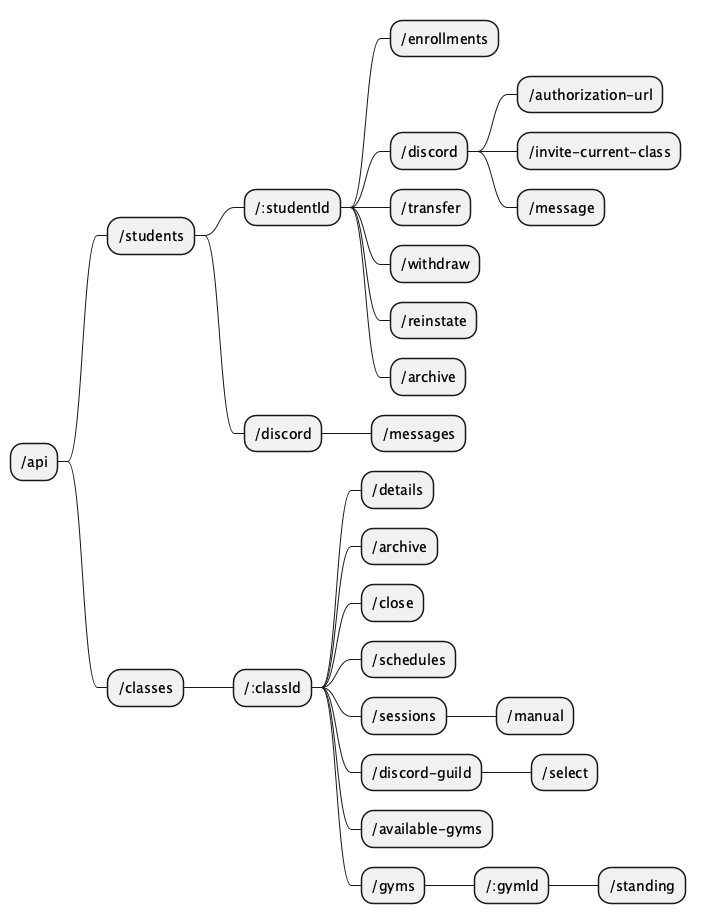
\includegraphics[width=0.96\textwidth,height=0.70\textheight,keepaspectratio]{diagrams/api-endpoint-backend-student-class.png}
    \caption{Các REST endpoint backend: học sinh và lớp học}
\end{figure}

\begin{figure}[H]
    \centering
    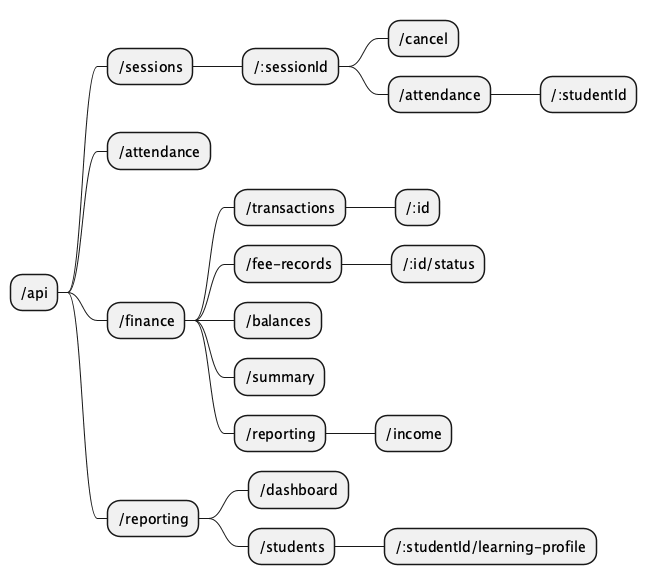
\includegraphics[width=0.96\textwidth,height=0.70\textheight,keepaspectratio]{diagrams/api-endpoint-backend-finance-reporting.png}
    \caption{Các REST endpoint backend: buổi học, điểm danh, tài chính và báo cáo}
\end{figure}

\subsection{Bảo mật và kiểm soát truy cập}

\begin{figure}[H]
    \centering
    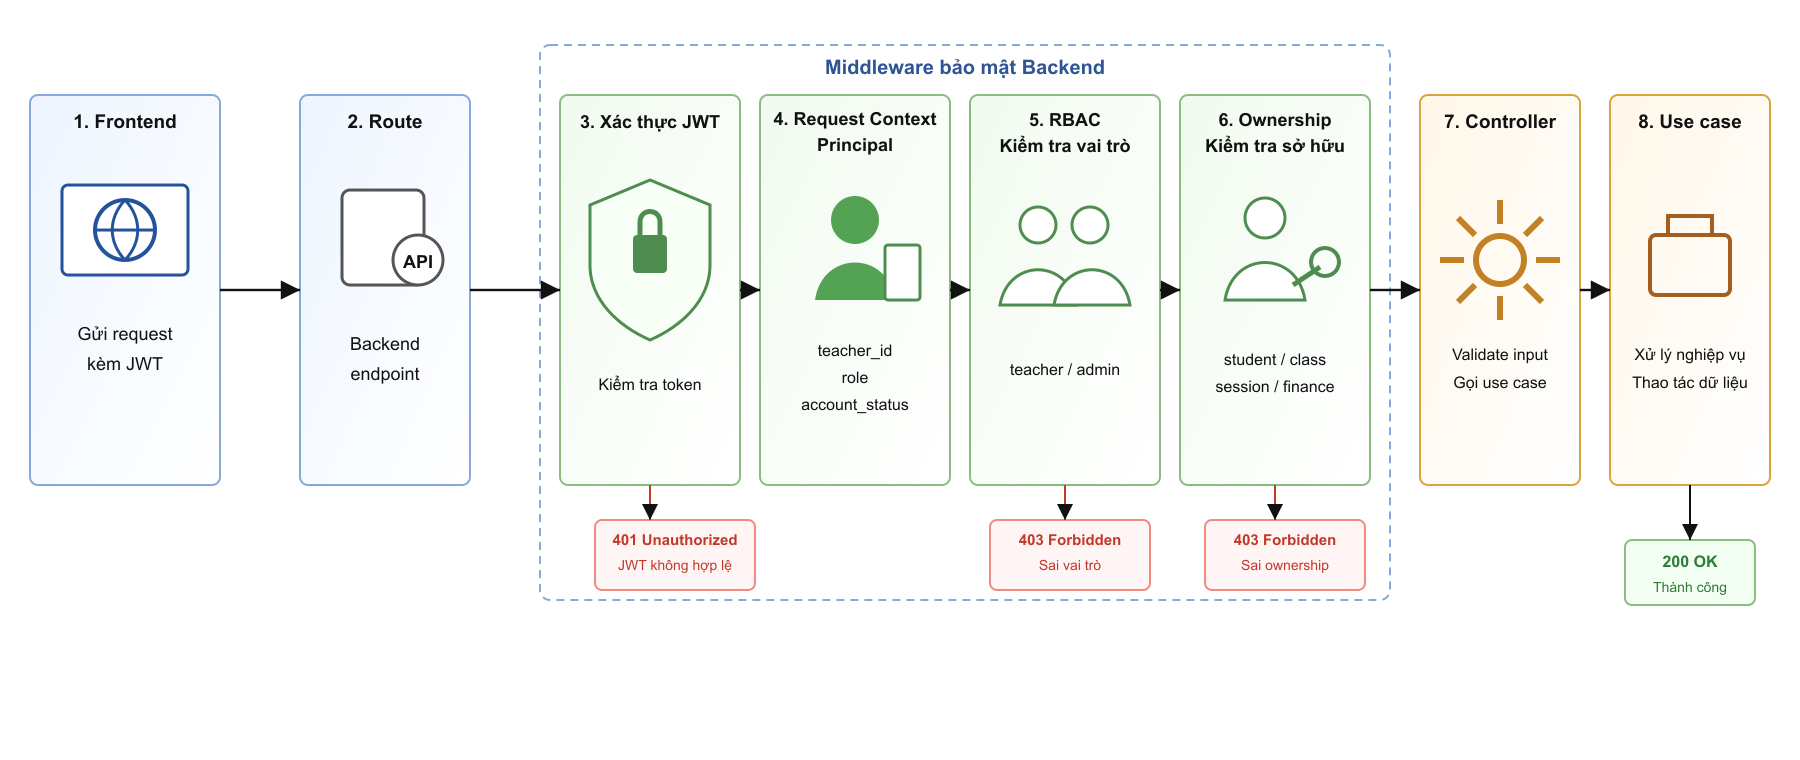
\includegraphics[width=0.96\textwidth,height=0.55\textheight,keepaspectratio]{diagrams/bao-mat-truy-cap.png}
    \caption{Luồng kiểm soát truy cập trước khi xử lý nghiệp vụ}
\end{figure}

Bảo mật được đặt ở lớp middleware của backend. Request từ frontend đi vào route
backend, sau đó phải lần lượt qua các bước xác thực JWT, tạo request context,
kiểm tra vai trò bằng RBAC và kiểm tra quyền sở hữu dữ liệu trước khi đến
controller.

\textbf{Quy tắc kiểm soát truy cập}
\begin{itemize}[leftmargin=*]
    \item Mọi request cần đăng nhập phải gửi JWT trong header \code{Authorization: Bearer <token>}.
    \item JWT authentication kiểm tra chữ ký, thời hạn và định dạng token. Nếu token thiếu hoặc không hợp lệ, request bị chặn với \code{401 Unauthorized}.
    \item Sau khi JWT hợp lệ, backend tạo principal trong request context, gồm \code{teacher\_id}, \code{role} và trạng thái tài khoản.
    \item RBAC kiểm tra vai trò có được phép đi vào route hay không. Admin được dùng route quản trị; teacher được dùng route nghiệp vụ của giáo viên. Sai vai trò bị chặn với \code{403 Forbidden}.
    \item Ownership check bảo đảm teacher chỉ truy cập dữ liệu thuộc phạm vi sở hữu của mình, gồm học sinh, lớp học, buổi học, hồ sơ tài chính và Gym được phân công. Sai phạm vi sở hữu cũng bị chặn với \code{403 Forbidden}.
\end{itemize}

\textbf{Mô tả luồng}
\begin{enumerate}[leftmargin=*]
    \item Frontend gửi HTTP request kèm JWT đến backend route.
    \item Route chuyển request qua middleware bảo mật.
    \item Middleware xác thực JWT và trích xuất principal.
    \item Hệ thống kiểm tra vai trò bằng RBAC.
    \item Với route truy cập dữ liệu theo giáo viên, hệ thống kiểm tra ownership.
    \item Request hợp lệ mới được chuyển đến controller và use case nghiệp vụ.
    \item Kết quả xử lý được trả về cho frontend.
\end{enumerate}

\subsection{Sơ đồ triển khai}

\begin{figure}[H]
    \centering
    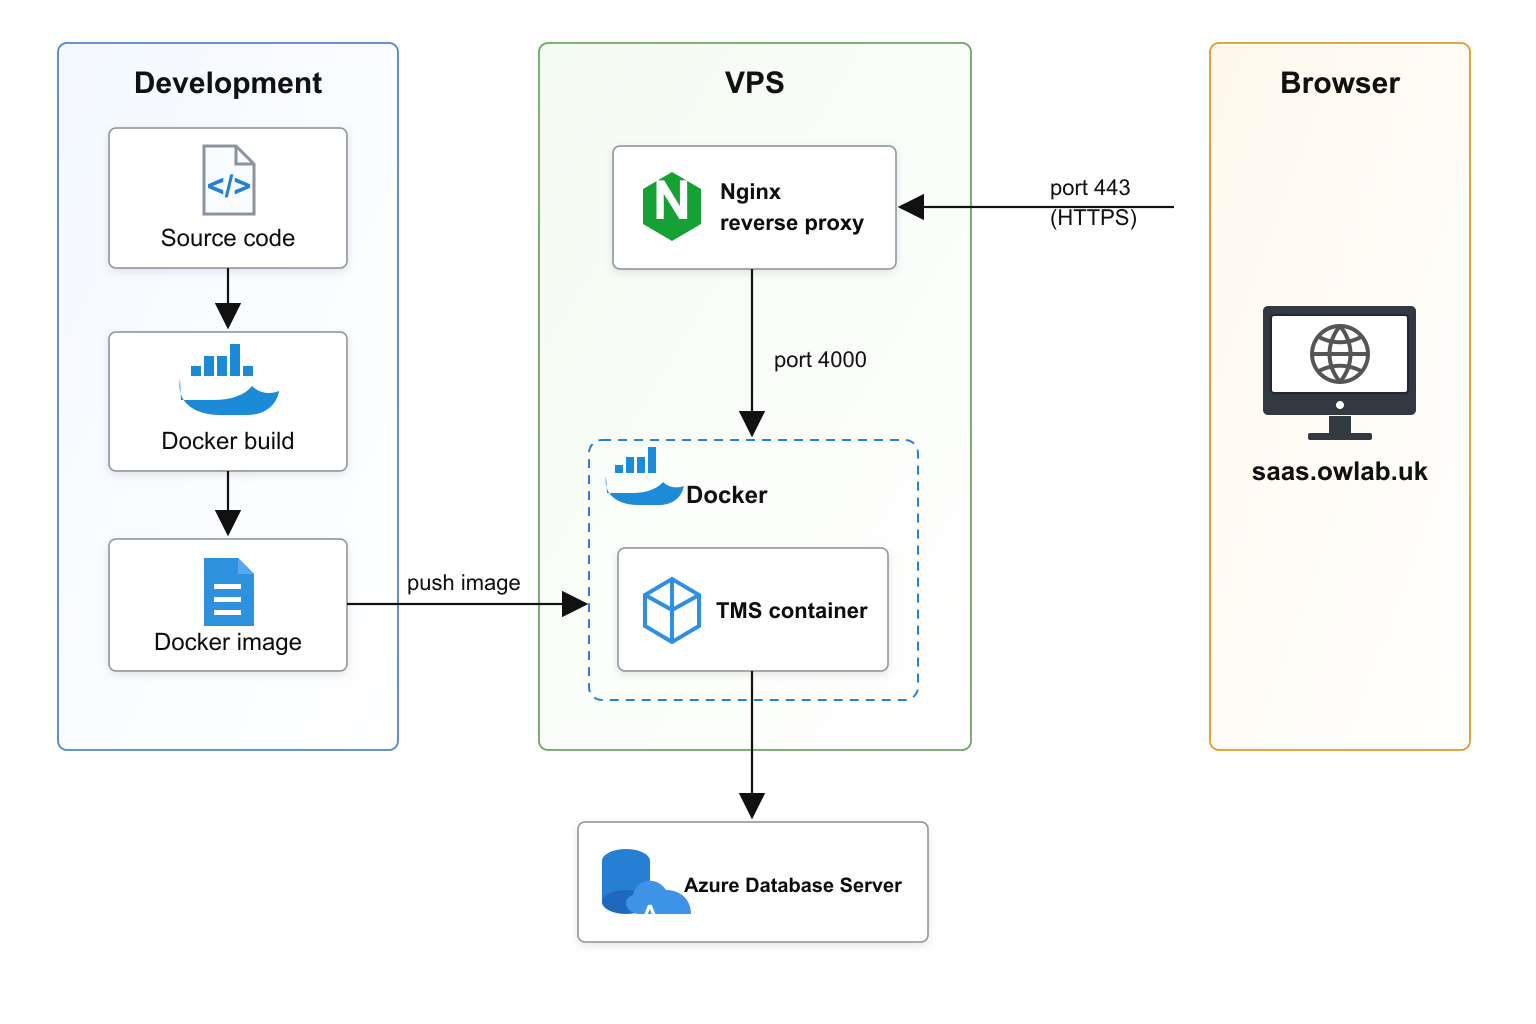
\includegraphics[width=0.92\textwidth,height=0.55\textheight,keepaspectratio]{diagrams/trien-khai-van-hanh.png}
    \caption{Sơ đồ triển khai phần mềm}
\end{figure}

\begin{enumerate}[leftmargin=*]
    \item Mã nguồn ở môi trường Development được build thành Docker image.
    \item Docker image được push từ môi trường Development sang VPS.
    \item Trên VPS, Docker chạy image này thành TMS container.
    \item Người dùng mở Browser và truy cập domain \code{saas.owlab.uk}.
    \item Request từ Browser đi vào VPS qua port 443.
    \item Nginx trên VPS nhận request ở port 443 và đóng vai trò reverse proxy.
    \item Nginx chuyển tiếp request vào TMS container qua port 4000.
    \item TMS container kết nối đến Azure Database Server để đọc và ghi dữ liệu TMS.
    \item TMS container xử lý request và trả kết quả ngược lại qua cùng đường đi.
\end{enumerate}

\clearpage

\setcounter{section}{5}
\section{Thiết kế cơ sở dữ liệu}

Phần này mô tả thiết kế cơ sở dữ liệu của hệ thống Tutor Management System
(TMS). Nội dung tập trung vào các lớp đối tượng được lưu trữ, quan hệ giữa
chúng và ý nghĩa của từng lớp trong dữ liệu nghiệp vụ.

\subsection{Sơ đồ lớp}

\begin{figure}[H]
    \centering
    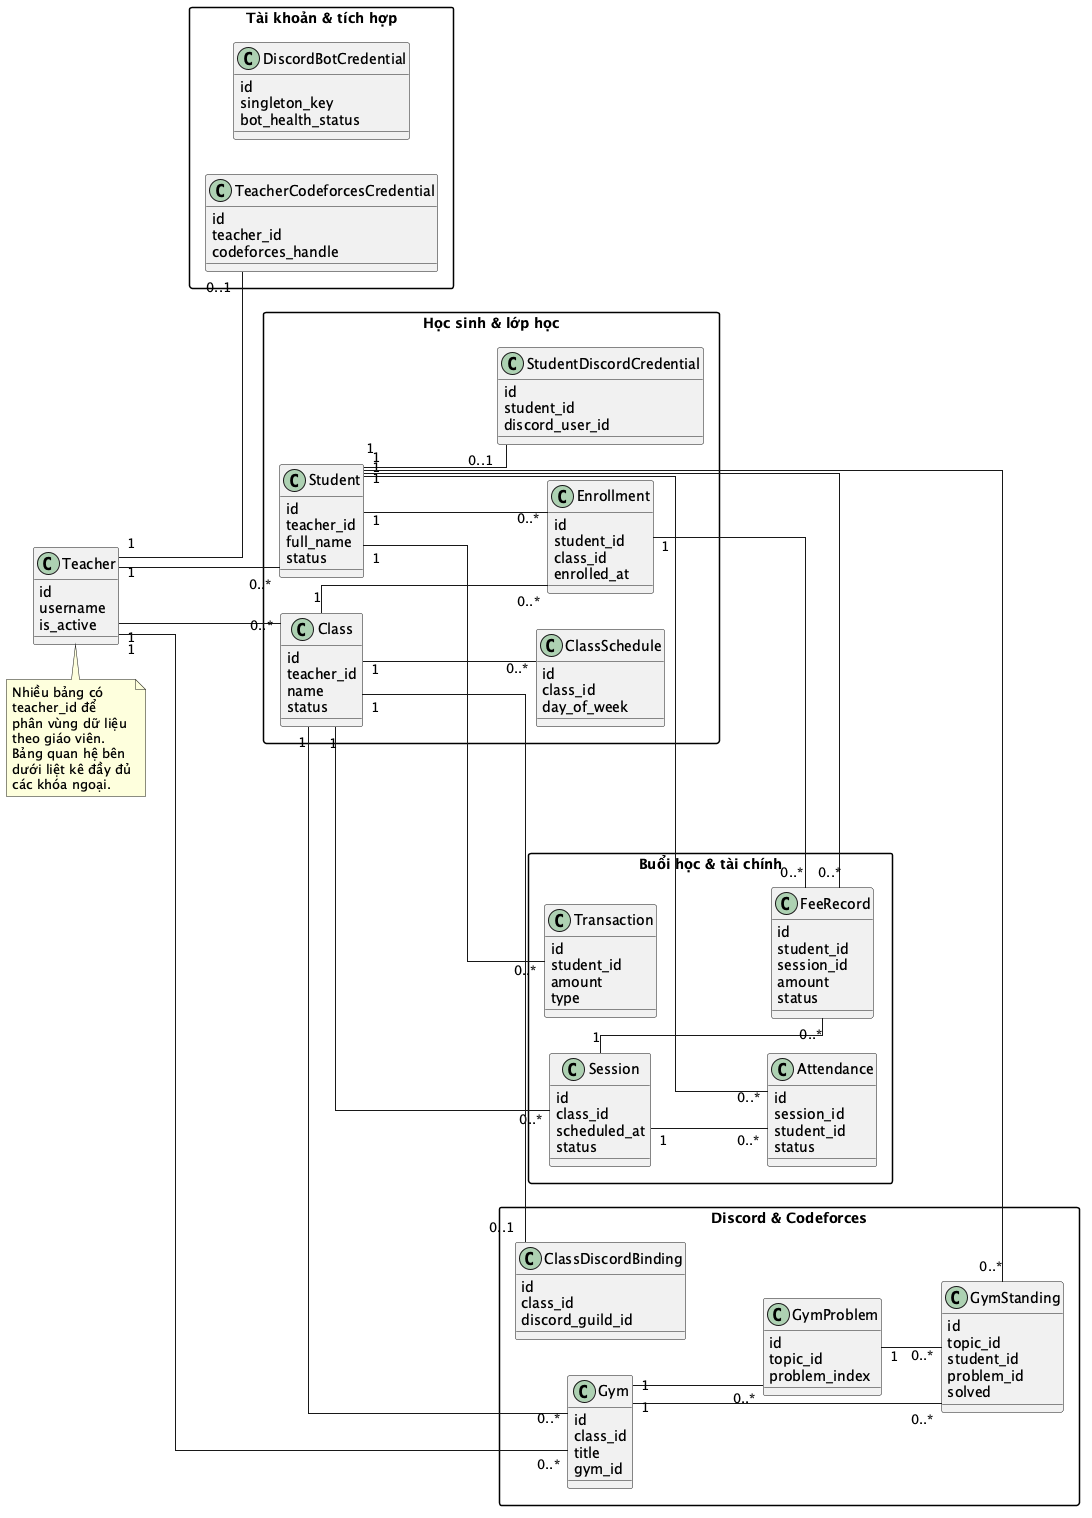
\includegraphics[width=0.98\textwidth,height=0.78\textheight,keepaspectratio]{diagrams/so-do-lop-co-so-du-lieu.png}
    \caption{Sơ đồ lớp dữ liệu của hệ thống TMS}
\end{figure}

Sơ đồ lớp thể hiện các đối tượng chính trong cơ sở dữ liệu. Các lớp trung tâm
là \code{Teacher}, \code{Student}, \code{Class}, \code{Session},
\code{Attendance}, \code{Transaction} và \code{FeeRecord}. Các lớp còn lại lưu
thông tin tích hợp Discord, Codeforces và cấu hình vận hành.

\subsection{Danh sách các lớp đối tượng}

\begin{longtable}{C{1cm} L{4.3cm} L{9.2cm}}
\toprule
\textbf{STT} & \textbf{Tên lớp} & \textbf{Mô tả} \\
\midrule
\endhead
1 & \code{teachers} & Lưu tài khoản giáo viên, trạng thái hoạt động và thông tin Discord đã xác minh. \\
2 & \code{teacher\_codeforces\_credential} & Lưu thông tin Codeforces API của giáo viên. \\
3 & \code{discord\_bot\_credentials} & Lưu cấu hình bot Discord dùng chung cho hệ thống. \\
4 & \code{students} & Lưu hồ sơ học sinh thuộc một giáo viên. \\
5 & \code{student\_discord\_credential} & Lưu thông tin liên kết Discord của học sinh. \\
6 & \code{classes} & Lưu lớp học, học phí mỗi buổi và trạng thái lớp. \\
7 & \code{enrollments} & Lưu lịch sử ghi danh học sinh vào lớp. \\
8 & \code{class\_schedules} & Lưu lịch học cố định của lớp theo ngày trong tuần. \\
9 & \code{sessions} & Lưu buổi học cụ thể của một lớp. \\
10 & \code{attendance} & Lưu kết quả điểm danh học sinh trong buổi học. \\
11 & \code{transactions} & Lưu giao dịch tài chính của học sinh. \\
12 & \code{fee\_records} & Lưu khoản phí phát sinh từ buổi học. \\
13 & \code{class\_discord\_bindings} & Lưu liên kết lớp học với Discord guild và channel. \\
14 & \code{gyms} & Lưu bài luyện tập Codeforces Gym gắn với giáo viên hoặc lớp. \\
15 & \code{gym\_problems} & Lưu danh sách bài trong một Gym. \\
16 & \code{gym\_standings} & Lưu kết quả làm bài của học sinh trong Gym. \\
\bottomrule
\end{longtable}

\subsection{Danh sách các quan hệ}

\begin{table}[H]
\small
\begin{tabularx}{\textwidth}{C{1cm} L{4.4cm} Y}
\toprule
\textbf{STT} & \textbf{Tên quan hệ} & \textbf{Mô tả} \\
\midrule
1 & Giáo viên -- Học sinh & Quan hệ 1--n: một giáo viên (\code{teachers}) quản lý nhiều học sinh (\code{students}). \\
2 & Giáo viên -- Lớp học & Quan hệ 1--n: một giáo viên quản lý nhiều lớp học (\code{classes}). \\
3 & Giáo viên -- Codeforces credential & Quan hệ 1--0..1: một giáo viên có tối đa một cấu hình Codeforces. \\
4 & Học sinh -- Discord credential & Quan hệ 1--0..1: một học sinh có tối đa một liên kết Discord. \\
5 & Học sinh -- Ghi danh & Quan hệ 1--n: một học sinh có nhiều bản ghi ghi danh (\code{enrollments}) theo thời gian. \\
6 & Lớp học -- Ghi danh & Quan hệ 1--n: một lớp có nhiều học sinh được ghi danh qua bảng \code{enrollments}. \\
7 & Lớp học -- Lịch học & Quan hệ 1--n: một lớp có nhiều lịch học cố định trong tuần. \\
8 & Lớp học -- Buổi học & Quan hệ 1--n: một lớp sinh ra nhiều buổi học (\code{sessions}). \\
9 & Buổi học -- Điểm danh & Quan hệ 1--n: một buổi học có nhiều bản ghi điểm danh. \\
10 & Học sinh -- Điểm danh & Quan hệ 1--n: một học sinh có nhiều bản ghi điểm danh theo các buổi học. \\
\bottomrule
\end{tabularx}
\end{table}

\begin{table}[H]
\small
\begin{tabularx}{\textwidth}{C{1cm} L{4.4cm} Y}
\toprule
\textbf{STT} & \textbf{Tên quan hệ} & \textbf{Mô tả} \\
\midrule
11 & Học sinh -- Giao dịch & Quan hệ 1--n: một học sinh có nhiều giao dịch tài chính. \\
12 & Học sinh -- Khoản phí & Quan hệ 1--n: một học sinh có nhiều khoản phí phát sinh. \\
13 & Buổi học -- Khoản phí & Quan hệ 1--n: một buổi học có thể sinh nhiều khoản phí cho học sinh tham gia. \\
14 & Ghi danh -- Khoản phí & Quan hệ 1--n: khoản phí gắn với bản ghi ghi danh tại thời điểm phát sinh. \\
15 & Lớp học -- Discord binding & Quan hệ 1--0..1: một lớp có tối đa một cấu hình Discord guild. \\
16 & Lớp học -- Gym & Quan hệ 1--n: một lớp có thể được gắn nhiều Codeforces Gym. \\
17 & Gym -- Bài tập & Quan hệ 1--n: một Gym có nhiều bài tập (\code{gym\_problems}). \\
18 & Gym -- Kết quả & Quan hệ 1--n: một Gym có nhiều dòng kết quả (\code{gym\_standings}). \\
19 & Học sinh -- Kết quả Gym & Quan hệ 1--n: một học sinh có nhiều kết quả trong Gym. \\
20 & Bài tập -- Kết quả Gym & Quan hệ 1--n: một bài tập có nhiều kết quả theo học sinh. \\
\bottomrule
\end{tabularx}
\end{table}

\subsection{Mô tả từng lớp đối tượng}

\subsubsection{Lớp teachers}
\begin{table}[H]\small\begin{tabularx}{\textwidth}{C{0.8cm} L{3cm} L{2.6cm} L{3cm} Y}
\toprule
\textbf{STT} & \textbf{Thuộc tính} & \textbf{Kiểu dữ liệu} & \textbf{Ràng buộc} & \textbf{Mô tả} \\
\midrule
1 & \code{id} & INT & PK, Auto Inc & Mã định danh giáo viên. \\
2 & \code{username} & VARCHAR(100) & NOT NULL, UNIQUE & Tên đăng nhập. \\
3 & \code{password\_hash} & TEXT & NOT NULL & Mật khẩu đã băm. \\
4 & \code{is\_active} & BIT & DEFAULT true & Trạng thái tài khoản. \\
5 & \code{discord\_user\_id} & VARCHAR(64) & NULL & Định danh Discord của giáo viên. \\
6 & \code{created\_at} & \datetimeoffset & DEFAULT now & Thời điểm tạo tài khoản. \\
\bottomrule
\end{tabularx}\end{table}

\subsubsection{Lớp teacher\_codeforces\_credential}
\begin{table}[H]\small\begin{tabularx}{\textwidth}{C{0.8cm} L{3cm} L{2.6cm} L{3cm} Y}
\toprule
\textbf{STT} & \textbf{Thuộc tính} & \textbf{Kiểu dữ liệu} & \textbf{Ràng buộc} & \textbf{Mô tả} \\
\midrule
1 & \code{id} & INT & PK, Auto Inc & Mã bản ghi credential. \\
2 & \code{teacher\_id} & INT & FK, UNIQUE & Giáo viên sở hữu credential. \\
3 & \code{codeforces\_handle} & VARCHAR(100) & NULL & Handle Codeforces của giáo viên. \\
4 & \code{codeforces\_api\_key} & TEXT & NULL, encrypted & API key Codeforces. \\
5 & \code{codeforces\_api\_secret} & TEXT & NULL, encrypted & API secret Codeforces. \\
6 & \code{updated\_at} & \datetimeoffset & DEFAULT now & Thời điểm cập nhật credential. \\
\bottomrule
\end{tabularx}\end{table}

\subsubsection{Lớp discord\_bot\_credentials}
\begin{table}[H]\small\begin{tabularx}{\textwidth}{C{0.8cm} L{3cm} L{2.6cm} L{3cm} Y}
\toprule
\textbf{STT} & \textbf{Thuộc tính} & \textbf{Kiểu dữ liệu} & \textbf{Ràng buộc} & \textbf{Mô tả} \\
\midrule
1 & \code{id} & INT & PK, Auto Inc & Mã cấu hình bot. \\
2 & \code{singleton\_key} & VARCHAR(32) & UNIQUE & Khóa bảo đảm chỉ có một cấu hình mặc định. \\
3 & \code{bot\_token} & TEXT & NOT NULL, encrypted & Token bot Discord. \\
4 & \code{client\_id} & VARCHAR(64) & NOT NULL & Client ID của Discord application. \\
5 & \code{client\_secret} & TEXT & encrypted & Client secret của Discord application. \\
6 & \code{bot\_health\_status} & VARCHAR(16) & DEFAULT unknown & Trạng thái kiểm tra bot. \\
\bottomrule
\end{tabularx}\end{table}

\subsubsection{Lớp students}
\begin{table}[H]\small\begin{tabularx}{\textwidth}{C{0.8cm} L{3cm} L{2.6cm} L{3cm} Y}
\toprule
\textbf{STT} & \textbf{Thuộc tính} & \textbf{Kiểu dữ liệu} & \textbf{Ràng buộc} & \textbf{Mô tả} \\
\midrule
1 & \code{id} & INT & PK, Auto Inc & Mã học sinh. \\
2 & \code{teacher\_id} & INT & FK, NOT NULL & Giáo viên quản lý học sinh. \\
3 & \code{full\_name} & VARCHAR(255) & NOT NULL & Họ tên học sinh. \\
4 & \code{codeforces\_handle} & VARCHAR(100) & UNIQUE theo giáo viên, NULL & Handle Codeforces của học sinh. \\
5 & \code{phone} & VARCHAR(20) & NULL & Số điện thoại. \\
6 & \code{status} & ENUM & DEFAULT active & Trạng thái học sinh. \\
7 & \code{archived\_at} & \datetimeoffset & NULL & Thời điểm lưu trữ học sinh. \\
\bottomrule
\end{tabularx}\end{table}

\subsubsection{Lớp student\_discord\_credential}
\begin{table}[H]\small\begin{tabularx}{\textwidth}{C{0.8cm} L{3cm} L{2.6cm} L{3cm} Y}
\toprule
\textbf{STT} & \textbf{Thuộc tính} & \textbf{Kiểu dữ liệu} & \textbf{Ràng buộc} & \textbf{Mô tả} \\
\midrule
1 & \code{id} & INT & PK, Auto Inc & Mã liên kết Discord. \\
2 & \code{student\_id} & INT & FK, UNIQUE & Học sinh được liên kết. \\
3 & \code{discord\_username} & NVARCHAR(100) & NULL & Tên hiển thị Discord. \\
4 & \code{discord\_user\_id} & VARCHAR(50) & NULL, INDEX & ID người dùng Discord. \\
5 & \code{guild\_id} & VARCHAR(50) & NULL, INDEX & Discord guild đang liên kết. \\
6 & \code{discord\_authorized\_at} & \datetimeoffset & NULL & Thời điểm học sinh cấp quyền Discord. \\
\bottomrule
\end{tabularx}\end{table}

\subsubsection{Lớp classes}
\begin{table}[H]\small\begin{tabularx}{\textwidth}{C{0.8cm} L{3cm} L{2.6cm} L{3cm} Y}
\toprule
\textbf{STT} & \textbf{Thuộc tính} & \textbf{Kiểu dữ liệu} & \textbf{Ràng buộc} & \textbf{Mô tả} \\
\midrule
1 & \code{id} & INT & PK, Auto Inc & Mã lớp học. \\
2 & \code{teacher\_id} & INT & FK, NOT NULL & Giáo viên sở hữu lớp. \\
3 & \code{name} & VARCHAR(255) & NOT NULL & Tên lớp học. \\
4 & \code{fee\_per\_session} & NUMERIC(12,0) & CHECK >= 0 & Học phí mỗi buổi. \\
5 & \code{status} & ENUM & DEFAULT active & Trạng thái lớp. \\
6 & \code{archived\_at} & \datetimeoffset & NULL & Thời điểm lưu trữ lớp. \\
\bottomrule
\end{tabularx}\end{table}

\subsubsection{Lớp enrollments}
\begin{table}[H]\small\begin{tabularx}{\textwidth}{C{0.8cm} L{3cm} L{2.6cm} L{3cm} Y}
\toprule
\textbf{STT} & \textbf{Thuộc tính} & \textbf{Kiểu dữ liệu} & \textbf{Ràng buộc} & \textbf{Mô tả} \\
\midrule
1 & \code{id} & INT & PK, Auto Inc & Mã ghi danh. \\
2 & \code{teacher\_id} & INT & FK, NOT NULL & Giáo viên sở hữu dữ liệu. \\
3 & \code{student\_id} & INT & FK, NOT NULL & Học sinh được ghi danh. \\
4 & \code{class\_id} & INT & FK, NOT NULL & Lớp được ghi danh. \\
5 & \code{enrolled\_at} & \datetimeoffset & DEFAULT now & Thời điểm vào lớp. \\
6 & \code{unenrolled\_at} & \datetimeoffset & NULL, CHECK & Thời điểm rút khỏi lớp. \\
\bottomrule
\end{tabularx}\end{table}

\subsubsection{Lớp class\_schedules}
\begin{table}[H]\small\begin{tabularx}{\textwidth}{C{0.8cm} L{3cm} L{2.6cm} L{3cm} Y}
\toprule
\textbf{STT} & \textbf{Thuộc tính} & \textbf{Kiểu dữ liệu} & \textbf{Ràng buộc} & \textbf{Mô tả} \\
\midrule
1 & \code{id} & INT & PK, Auto Inc & Mã lịch học. \\
2 & \code{teacher\_id} & INT & FK, NOT NULL & Giáo viên sở hữu dữ liệu. \\
3 & \code{class\_id} & INT & FK, NOT NULL & Lớp áp dụng lịch học. \\
4 & \code{day\_of\_week} & SMALLINT & CHECK 0--6 & Ngày học trong tuần. \\
5 & \code{start\_time} & TIME & NOT NULL & Giờ bắt đầu. \\
6 & \code{end\_time} & TIME & CHECK > start & Giờ kết thúc. \\
\bottomrule
\end{tabularx}\end{table}

\subsubsection{Lớp sessions}
\begin{table}[H]\small\begin{tabularx}{\textwidth}{C{0.8cm} L{3cm} L{2.6cm} L{3cm} Y}
\toprule
\textbf{STT} & \textbf{Thuộc tính} & \textbf{Kiểu dữ liệu} & \textbf{Ràng buộc} & \textbf{Mô tả} \\
\midrule
1 & \code{id} & INT & PK, Auto Inc & Mã buổi học. \\
2 & \code{teacher\_id} & INT & FK, NOT NULL & Giáo viên sở hữu dữ liệu. \\
3 & \code{class\_id} & INT & FK, NOT NULL & Lớp của buổi học. \\
4 & \code{scheduled\_at} & \datetimeoffset & NOT NULL & Thời điểm bắt đầu buổi học. \\
5 & \code{end\_time} & TIME & NULL, CHECK & Giờ kết thúc nếu có. \\
6 & \code{status} & ENUM & DEFAULT scheduled & Trạng thái buổi học. \\
7 & \code{cancelled\_at} & \datetimeoffset & NULL & Thời điểm hủy buổi học. \\
\bottomrule
\end{tabularx}\end{table}

\subsubsection{Lớp attendance}
\begin{table}[H]\small\begin{tabularx}{\textwidth}{C{0.8cm} L{3cm} L{2.6cm} L{3cm} Y}
\toprule
\textbf{STT} & \textbf{Thuộc tính} & \textbf{Kiểu dữ liệu} & \textbf{Ràng buộc} & \textbf{Mô tả} \\
\midrule
1 & \code{id} & INT & PK, Auto Inc & Mã điểm danh. \\
2 & \code{teacher\_id} & INT & FK, NOT NULL & Giáo viên sở hữu dữ liệu. \\
3 & \code{session\_id} & INT & FK, UNIQUE theo student & Buổi học được điểm danh. \\
4 & \code{student\_id} & INT & FK, UNIQUE theo session & Học sinh được điểm danh. \\
5 & \code{status} & ENUM & NOT NULL & Kết quả điểm danh. \\
6 & \code{source} & ENUM & DEFAULT system & Nguồn tạo điểm danh. \\
7 & \code{overridden\_at} & \datetimeoffset & NULL, CHECK & Thời điểm giáo viên ghi đè. \\
\bottomrule
\end{tabularx}\end{table}

\subsubsection{Lớp transactions}
\begin{table}[H]\small\begin{tabularx}{\textwidth}{C{0.8cm} L{3cm} L{2.6cm} L{3cm} Y}
\toprule
\textbf{STT} & \textbf{Thuộc tính} & \textbf{Kiểu dữ liệu} & \textbf{Ràng buộc} & \textbf{Mô tả} \\
\midrule
1 & \code{id} & INT & PK, Auto Inc & Mã giao dịch. \\
2 & \code{teacher\_id} & INT & FK, NOT NULL & Giáo viên sở hữu dữ liệu. \\
3 & \code{student\_id} & INT & FK, NOT NULL & Học sinh phát sinh giao dịch. \\
4 & \code{amount} & NUMERIC(12,0) & CHECK != 0 & Số tiền giao dịch. \\
5 & \code{type} & ENUM & CHECK dấu amount & Loại giao dịch: payment hoặc refund. \\
6 & \code{recorded\_at} & \datetimeoffset & DEFAULT now & Thời điểm ghi nhận giao dịch. \\
7 & \code{notes} & NVARCHAR(MAX) & NULL & Ghi chú giao dịch. \\
\bottomrule
\end{tabularx}\end{table}

\subsubsection{Lớp fee\_records}
\begin{table}[H]\small\begin{tabularx}{\textwidth}{C{0.8cm} L{3cm} L{2.6cm} L{3cm} Y}
\toprule
\textbf{STT} & \textbf{Thuộc tính} & \textbf{Kiểu dữ liệu} & \textbf{Ràng buộc} & \textbf{Mô tả} \\
\midrule
1 & \code{id} & INT & PK, Auto Inc & Mã khoản phí. \\
2 & \code{teacher\_id} & INT & FK, NOT NULL & Giáo viên sở hữu dữ liệu. \\
3 & \code{student\_id} & INT & FK, UNIQUE theo session & Học sinh chịu phí. \\
4 & \code{session\_id} & INT & FK, UNIQUE theo student & Buổi học phát sinh phí. \\
5 & \code{enrollment\_id} & INT & FK, NOT NULL & Bản ghi ghi danh liên quan. \\
6 & \code{amount} & NUMERIC(12,0) & CHECK > 0 & Số tiền phải thu. \\
7 & \code{status} & ENUM & DEFAULT active & Trạng thái khoản phí. \\
\bottomrule
\end{tabularx}\end{table}

\subsubsection{Lớp class\_discord\_bindings}
\begin{table}[H]\small\begin{tabularx}{\textwidth}{C{0.8cm} L{3cm} L{2.6cm} L{3cm} Y}
\toprule
\textbf{STT} & \textbf{Thuộc tính} & \textbf{Kiểu dữ liệu} & \textbf{Ràng buộc} & \textbf{Mô tả} \\
\midrule
1 & \code{id} & INT & PK, Auto Inc & Mã cấu hình Discord của lớp. \\
2 & \code{teacher\_id} & INT & FK, NOT NULL & Giáo viên sở hữu cấu hình. \\
3 & \code{class\_id} & INT & FK, UNIQUE & Lớp được liên kết Discord. \\
4 & \code{discord\_guild\_id} & VARCHAR(50) & UNIQUE theo teacher & Discord guild của lớp. \\
5 & \code{name} & NVARCHAR(255) & NULL & Tên guild. \\
6 & \code{attendance\_voice\_channel\_id} & VARCHAR(50) & NULL & Voice channel dùng để điểm danh. \\
7 & \code{notification\_channel\_id} & VARCHAR(50) & NULL & Channel gửi thông báo. \\
\bottomrule
\end{tabularx}\end{table}

\subsubsection{Lớp gyms}
\begin{table}[H]\small\begin{tabularx}{\textwidth}{C{0.8cm} L{3cm} L{2.6cm} L{3cm} Y}
\toprule
\textbf{STT} & \textbf{Thuộc tính} & \textbf{Kiểu dữ liệu} & \textbf{Ràng buộc} & \textbf{Mô tả} \\
\midrule
1 & \code{id} & INT & PK, Auto Inc & Mã Gym nội bộ. \\
2 & \code{teacher\_id} & INT & FK, NOT NULL & Giáo viên sở hữu Gym. \\
3 & \code{class\_id} & INT & FK, NULL & Lớp được gắn Gym nếu có. \\
4 & \code{title} & VARCHAR(255) & NOT NULL & Tiêu đề Gym. \\
5 & \code{gym\_link} & TEXT & NOT NULL & Đường dẫn Gym trên Codeforces. \\
6 & \code{gym\_id} & VARCHAR(50) & UNIQUE theo phạm vi & Mã Gym trên Codeforces. \\
7 & \code{pull\_interval\_minutes} & INT & CHECK > 0 & Chu kỳ đồng bộ kết quả. \\
\bottomrule
\end{tabularx}\end{table}

\subsubsection{Lớp gym\_problems}
\begin{table}[H]\small\begin{tabularx}{\textwidth}{C{0.8cm} L{3cm} L{2.6cm} L{3cm} Y}
\toprule
\textbf{STT} & \textbf{Thuộc tính} & \textbf{Kiểu dữ liệu} & \textbf{Ràng buộc} & \textbf{Mô tả} \\
\midrule
1 & \code{id} & INT & PK, Auto Inc & Mã bài tập. \\
2 & \code{teacher\_id} & INT & FK, NOT NULL & Giáo viên sở hữu dữ liệu. \\
3 & \code{topic\_id} & INT & FK, NOT NULL & Gym chứa bài tập. \\
4 & \code{problem\_index} & VARCHAR(10) & UNIQUE theo Gym & Chỉ số bài trong Gym. \\
5 & \code{problem\_name} & NVARCHAR(255) & NULL & Tên bài tập. \\
\bottomrule
\end{tabularx}\end{table}

\subsubsection{Lớp gym\_standings}
\begin{table}[H]\small\begin{tabularx}{\textwidth}{C{0.8cm} L{3cm} L{2.6cm} L{3cm} Y}
\toprule
\textbf{STT} & \textbf{Thuộc tính} & \textbf{Kiểu dữ liệu} & \textbf{Ràng buộc} & \textbf{Mô tả} \\
\midrule
1 & \code{id} & INT & PK, Auto Inc & Mã kết quả Gym. \\
2 & \code{teacher\_id} & INT & FK, NOT NULL & Giáo viên sở hữu dữ liệu. \\
3 & \code{topic\_id} & INT & FK, UNIQUE theo student/problem & Gym chứa kết quả. \\
4 & \code{student\_id} & INT & FK, UNIQUE theo topic/problem & Học sinh có kết quả. \\
5 & \code{problem\_id} & INT & FK, UNIQUE theo topic/student & Bài tập tương ứng. \\
6 & \code{solved} & BIT & DEFAULT false & Học sinh đã giải bài hay chưa. \\
7 & \code{penalty\_minutes} & INT & NULL & Thời gian phạt nếu có. \\
8 & \code{pulled\_at} & \datetimeoffset & DEFAULT now & Thời điểm kéo kết quả. \\
\bottomrule
\end{tabularx}\end{table}

\input{../section7/section7.txt}

\setcounter{section}{7}
\section{Phân chia công việc}

\begin{itemize}[leftmargin=*]
    \item \textbf{Lê Quang Trung -- 24521883}
    \begin{itemize}
        \item Nhóm trưởng, điều phối công việc chung của nhóm.
        \item Thiết kế kiến trúc hệ thống.
        \item Thiết kế luồng đồng bộ dữ liệu với hệ thống ngoài.
        \item Thiết kế API endpoint và cơ chế tích hợp giữa frontend với backend.
        \item Thiết kế mô hình dữ liệu.
        \item Cài đặt, triển khai hệ thống.
        \item Viết báo cáo về kiến trúc hệ thống.
        \item Viết báo cáo về thiết kế cơ sở dữ liệu.
        \item \textbf{Kết quả: Hoàn thành.}
    \end{itemize}

    \item \textbf{Nguyễn Thành Sơn -- 24521532}
    \begin{itemize}
        \item Thiết kế module classroom.
        \item Phân tích nghiệp vụ quản lý lớp học.
        \item Thiết kế chức năng quản lý lớp, lịch học và buổi học.
        \item Viết báo cáo về đặc tả và phân tích yêu cầu chức năng phần mềm.
        \item Viết báo cáo về mô hình hóa yêu cầu chức năng thuộc module classroom.
        \item \textbf{Kết quả: Hoàn thành.}
    \end{itemize}

    \item \textbf{Đinh Mạnh Hùng -- 24520014}
    \begin{itemize}
        \item Thiết kế module student và finance.
        \item Phân tích nghiệp vụ quản lý học sinh.
        \item Thiết kế chức năng ghi danh, chuyển lớp và lưu trữ học sinh.
        \item Thiết kế chức năng giao dịch, học phí, công nợ và báo cáo tài chính.
        \item Viết báo cáo về thiết kế giao diện cho các chức năng của hệ thống.
        \item Viết báo cáo về mô hình hóa yêu cầu chức năng thuộc module student và finance.
        \item \textbf{Kết quả: Hoàn thành.}
    \end{itemize}

    \item \textbf{Trần Vạn Tấn -- 23521407}
    \begin{itemize}
        \item Phân tích nghiệp vụ đăng nhập, đăng ký và quản lý phiên làm việc.
        \item Thiết kế module account và system.
        \item Thiết kế chức năng quản lý tài khoản giáo viên.
        \item Thiết kế slide thuyết trình.
        \item Viết báo cáo về tổng quan đề tài.
        \item Viết báo cáo về xác định và thu thập yêu cầu.
        \item Viết báo cáo về mô hình hóa yêu cầu chức năng thuộc module account và system.
        \item Thuyết trình báo cáo.
        \item \textbf{Kết quả: Hoàn thành.}
    \end{itemize}
\end{itemize}

\end{document}
